\documentclass[twoside]{book}

% Packages required by doxygen
\usepackage{fixltx2e}
\usepackage{calc}
\usepackage{doxygen}
\usepackage{graphicx}
\usepackage[utf8]{inputenc}
\usepackage{makeidx}
\usepackage{multicol}
\usepackage{multirow}
\PassOptionsToPackage{warn}{textcomp}
\usepackage{textcomp}
\usepackage[nointegrals]{wasysym}
\usepackage[table]{xcolor}

% Font selection
\usepackage[T1]{fontenc}
\usepackage{mathptmx}
\usepackage[scaled=.90]{helvet}
\usepackage{courier}
\usepackage{amssymb}
\usepackage{sectsty}
\renewcommand{\familydefault}{\sfdefault}
\allsectionsfont{%
  \fontseries{bc}\selectfont%
  \color{darkgray}%
}
\renewcommand{\DoxyLabelFont}{%
  \fontseries{bc}\selectfont%
  \color{darkgray}%
}
\newcommand{\+}{\discretionary{\mbox{\scriptsize$\hookleftarrow$}}{}{}}

% Page & text layout
\usepackage{geometry}
\geometry{%
  a4paper,%
  top=2.5cm,%
  bottom=2.5cm,%
  left=2.5cm,%
  right=2.5cm%
}
\tolerance=750
\hfuzz=15pt
\hbadness=750
\setlength{\emergencystretch}{15pt}
\setlength{\parindent}{0cm}
\setlength{\parskip}{0.2cm}
\makeatletter
\renewcommand{\paragraph}{%
  \@startsection{paragraph}{4}{0ex}{-1.0ex}{1.0ex}{%
    \normalfont\normalsize\bfseries\SS@parafont%
  }%
}
\renewcommand{\subparagraph}{%
  \@startsection{subparagraph}{5}{0ex}{-1.0ex}{1.0ex}{%
    \normalfont\normalsize\bfseries\SS@subparafont%
  }%
}
\makeatother

% Headers & footers
\usepackage{fancyhdr}
\pagestyle{fancyplain}
\fancyhead[LE]{\fancyplain{}{\bfseries\thepage}}
\fancyhead[CE]{\fancyplain{}{}}
\fancyhead[RE]{\fancyplain{}{\bfseries\leftmark}}
\fancyhead[LO]{\fancyplain{}{\bfseries\rightmark}}
\fancyhead[CO]{\fancyplain{}{}}
\fancyhead[RO]{\fancyplain{}{\bfseries\thepage}}
\fancyfoot[LE]{\fancyplain{}{}}
\fancyfoot[CE]{\fancyplain{}{}}
\fancyfoot[RE]{\fancyplain{}{\bfseries\scriptsize Generated on Thu Feb 16 2017 12\+:56\+:10 for Q\+C\+\_\+\+Dve\+\_\+\+Core by Doxygen }}
\fancyfoot[LO]{\fancyplain{}{\bfseries\scriptsize Generated on Thu Feb 16 2017 12\+:56\+:10 for Q\+C\+\_\+\+Dve\+\_\+\+Core by Doxygen }}
\fancyfoot[CO]{\fancyplain{}{}}
\fancyfoot[RO]{\fancyplain{}{}}
\renewcommand{\footrulewidth}{0.4pt}
\renewcommand{\chaptermark}[1]{%
  \markboth{#1}{}%
}
\renewcommand{\sectionmark}[1]{%
  \markright{\thesection\ #1}%
}

% Indices & bibliography
\usepackage{natbib}
\usepackage[titles]{tocloft}
\setcounter{tocdepth}{3}
\setcounter{secnumdepth}{5}
\makeindex

% Hyperlinks (required, but should be loaded last)
\usepackage{ifpdf}
\ifpdf
  \usepackage[pdftex,pagebackref=true]{hyperref}
\else
  \usepackage[ps2pdf,pagebackref=true]{hyperref}
\fi
\hypersetup{%
  colorlinks=true,%
  linkcolor=blue,%
  citecolor=blue,%
  unicode%
}

% Custom commands
\newcommand{\clearemptydoublepage}{%
  \newpage{\pagestyle{empty}\cleardoublepage}%
}


%===== C O N T E N T S =====

\begin{document}

% Titlepage & ToC
\hypersetup{pageanchor=false,
             bookmarks=true,
             bookmarksnumbered=true,
             pdfencoding=unicode
            }
\pagenumbering{roman}
\begin{titlepage}
\vspace*{7cm}
\begin{center}%
{\Large Q\+C\+\_\+\+Dve\+\_\+\+Core \\[1ex]\large 0.\+5 }\\
\vspace*{1cm}
{\large Generated by Doxygen 1.8.8}\\
\vspace*{0.5cm}
{\small Thu Feb 16 2017 12:56:10}\\
\end{center}
\end{titlepage}
\clearemptydoublepage
\tableofcontents
\clearemptydoublepage
\pagenumbering{arabic}
\hypersetup{pageanchor=true}

%--- Begin generated contents ---
\chapter{Hierarchical Index}
\section{Class Hierarchy}
This inheritance list is sorted roughly, but not completely, alphabetically\+:\begin{DoxyCompactList}
\item \contentsline{section}{Q\+C\+Business\+Calendar}{\pageref{class_q_c_business_calendar}}{}
\item \contentsline{section}{Q\+C\+Curve$<$ T $>$}{\pageref{class_q_c_curve}}{}
\item \contentsline{section}{Q\+C\+Date}{\pageref{class_q_c_date}}{}
\item \contentsline{section}{Q\+C\+Interest\+Rate}{\pageref{class_q_c_interest_rate}}{}
\item \contentsline{section}{Q\+C\+Interest\+Rate\+Curve}{\pageref{class_q_c_interest_rate_curve}}{}
\begin{DoxyCompactList}
\item \contentsline{section}{Q\+C\+Projecting\+Interest\+Rate\+Curve}{\pageref{class_q_c_projecting_interest_rate_curve}}{}
\item \contentsline{section}{Q\+C\+Zero\+Coupon\+Curve}{\pageref{class_q_c_zero_coupon_curve}}{}
\begin{DoxyCompactList}
\item \contentsline{section}{Q\+C\+Zero\+Coupon\+Discount\+Factor\+Curve}{\pageref{class_q_c_zero_coupon_discount_factor_curve}}{}
\item \contentsline{section}{Q\+C\+Zero\+Coupon\+Interest\+Rate\+Curve}{\pageref{class_q_c_zero_coupon_interest_rate_curve}}{}
\end{DoxyCompactList}
\end{DoxyCompactList}
\item \contentsline{section}{Q\+C\+Interest\+Rate\+Leg}{\pageref{class_q_c_interest_rate_leg}}{}
\item \contentsline{section}{Q\+C\+Interest\+Rate\+Payoff}{\pageref{class_q_c_interest_rate_payoff}}{}
\begin{DoxyCompactList}
\item \contentsline{section}{Q\+C\+Fixed\+Rate\+Payoff}{\pageref{class_q_c_fixed_rate_payoff}}{}
\item \contentsline{section}{Q\+C\+Floating\+Rate\+Payoff}{\pageref{class_q_c_floating_rate_payoff}}{}
\item \contentsline{section}{Q\+C\+Icp\+Clf\+Payoff}{\pageref{class_q_c_icp_clf_payoff}}{}
\item \contentsline{section}{Q\+C\+Icp\+Clp\+Payoff}{\pageref{class_q_c_icp_clp_payoff}}{}
\end{DoxyCompactList}
\item \contentsline{section}{Q\+C\+Interest\+Rate\+Periods\+Factory}{\pageref{class_q_c_interest_rate_periods_factory}}{}
\item \contentsline{section}{Q\+C\+Interpolator}{\pageref{class_q_c_interpolator}}{}
\begin{DoxyCompactList}
\item \contentsline{section}{Q\+C\+Clamped\+Spline}{\pageref{class_q_c_clamped_spline}}{}
\item \contentsline{section}{Q\+C\+Linear\+Interpolator}{\pageref{class_q_c_linear_interpolator}}{}
\item \contentsline{section}{Q\+C\+Log\+Linear\+Interpolator}{\pageref{class_q_c_log_linear_interpolator}}{}
\end{DoxyCompactList}
\item \contentsline{section}{Q\+C\+Test}{\pageref{class_q_c_test}}{}
\item \contentsline{section}{Q\+C\+Wealth\+Factor}{\pageref{class_q_c_wealth_factor}}{}
\begin{DoxyCompactList}
\item \contentsline{section}{Q\+C\+Compound\+Wf}{\pageref{class_q_c_compound_wf}}{}
\item \contentsline{section}{Q\+C\+Continous\+Wf}{\pageref{class_q_c_continous_wf}}{}
\item \contentsline{section}{Q\+C\+Linear\+Wf}{\pageref{class_q_c_linear_wf}}{}
\end{DoxyCompactList}
\item \contentsline{section}{Q\+C\+Year\+Fraction}{\pageref{class_q_c_year_fraction}}{}
\begin{DoxyCompactList}
\item \contentsline{section}{Q\+C30360}{\pageref{class_q_c30360}}{}
\item \contentsline{section}{Q\+C\+Act360}{\pageref{class_q_c_act360}}{}
\item \contentsline{section}{Q\+C\+Act365}{\pageref{class_q_c_act365}}{}
\item \contentsline{section}{Q\+C\+Act\+Act}{\pageref{class_q_c_act_act}}{}
\end{DoxyCompactList}
\end{DoxyCompactList}

\chapter{Class Index}
\section{Class List}
Here are the classes, structs, unions and interfaces with brief descriptions\+:\begin{DoxyCompactList}
\item\contentsline{section}{\hyperlink{class_q_c30360}{Q\+C30360} \\*La clase \hyperlink{class_q_c30360}{Q\+C30360} implementa el método 30/360. Hereda de la clase abstracta \hyperlink{class_q_c_year_fraction}{Q\+C\+Year\+Fraction} }{\pageref{class_q_c30360}}{}
\item\contentsline{section}{\hyperlink{class_q_c_act360}{Q\+C\+Act360} \\*La clase \hyperlink{class_q_c_act360}{Q\+C\+Act360} implementa el método Act/360. Hereda de la clase abstracta \hyperlink{class_q_c_year_fraction}{Q\+C\+Year\+Fraction} }{\pageref{class_q_c_act360}}{}
\item\contentsline{section}{\hyperlink{class_q_c_act365}{Q\+C\+Act365} \\*La clase \hyperlink{class_q_c_act360}{Q\+C\+Act360} implementa el método Act/365. Hereda de la clase abstracta \hyperlink{class_q_c_year_fraction}{Q\+C\+Year\+Fraction} }{\pageref{class_q_c_act365}}{}
\item\contentsline{section}{\hyperlink{class_q_c_act_act}{Q\+C\+Act\+Act} \\*La clase \hyperlink{class_q_c_act360}{Q\+C\+Act360} implementa el método Act/\+Act. Hereda de la clase abstracta \hyperlink{class_q_c_year_fraction}{Q\+C\+Year\+Fraction} }{\pageref{class_q_c_act_act}}{}
\item\contentsline{section}{\hyperlink{class_q_c_business_calendar}{Q\+C\+Business\+Calendar} \\*La clase \hyperlink{class_q_c_business_calendar}{Q\+C\+Business\+Calendar} representa días feriados de una jurisdicción }{\pageref{class_q_c_business_calendar}}{}
\item\contentsline{section}{\hyperlink{class_q_c_clamped_spline}{Q\+C\+Clamped\+Spline} }{\pageref{class_q_c_clamped_spline}}{}
\item\contentsline{section}{\hyperlink{class_q_c_compound_wf}{Q\+C\+Compound\+Wf} }{\pageref{class_q_c_compound_wf}}{}
\item\contentsline{section}{\hyperlink{class_q_c_continous_wf}{Q\+C\+Continous\+Wf} }{\pageref{class_q_c_continous_wf}}{}
\item\contentsline{section}{\hyperlink{class_q_c_curve}{Q\+C\+Curve$<$ T $>$} }{\pageref{class_q_c_curve}}{}
\item\contentsline{section}{\hyperlink{class_q_c_date}{Q\+C\+Date} \\*\hyperlink{class_q_c_date}{Q\+C\+Date} es la implementación de Q\+Code de una clase para manejar fechas }{\pageref{class_q_c_date}}{}
\item\contentsline{section}{\hyperlink{class_q_c_fixed_rate_payoff}{Q\+C\+Fixed\+Rate\+Payoff} }{\pageref{class_q_c_fixed_rate_payoff}}{}
\item\contentsline{section}{\hyperlink{class_q_c_floating_rate_payoff}{Q\+C\+Floating\+Rate\+Payoff} }{\pageref{class_q_c_floating_rate_payoff}}{}
\item\contentsline{section}{\hyperlink{class_q_c_icp_clf_payoff}{Q\+C\+Icp\+Clf\+Payoff} }{\pageref{class_q_c_icp_clf_payoff}}{}
\item\contentsline{section}{\hyperlink{class_q_c_icp_clp_payoff}{Q\+C\+Icp\+Clp\+Payoff} }{\pageref{class_q_c_icp_clp_payoff}}{}
\item\contentsline{section}{\hyperlink{class_q_c_interest_rate}{Q\+C\+Interest\+Rate} }{\pageref{class_q_c_interest_rate}}{}
\item\contentsline{section}{\hyperlink{class_q_c_interest_rate_curve}{Q\+C\+Interest\+Rate\+Curve} \\*Clase base abstracta para todas las curvas de tasas de interés }{\pageref{class_q_c_interest_rate_curve}}{}
\item\contentsline{section}{\hyperlink{class_q_c_interest_rate_leg}{Q\+C\+Interest\+Rate\+Leg} }{\pageref{class_q_c_interest_rate_leg}}{}
\item\contentsline{section}{\hyperlink{class_q_c_interest_rate_payoff}{Q\+C\+Interest\+Rate\+Payoff} }{\pageref{class_q_c_interest_rate_payoff}}{}
\item\contentsline{section}{\hyperlink{class_q_c_interest_rate_periods_factory}{Q\+C\+Interest\+Rate\+Periods\+Factory} }{\pageref{class_q_c_interest_rate_periods_factory}}{}
\item\contentsline{section}{\hyperlink{class_q_c_interpolator}{Q\+C\+Interpolator} }{\pageref{class_q_c_interpolator}}{}
\item\contentsline{section}{\hyperlink{class_q_c_linear_interpolator}{Q\+C\+Linear\+Interpolator} }{\pageref{class_q_c_linear_interpolator}}{}
\item\contentsline{section}{\hyperlink{class_q_c_linear_wf}{Q\+C\+Linear\+Wf} }{\pageref{class_q_c_linear_wf}}{}
\item\contentsline{section}{\hyperlink{class_q_c_log_linear_interpolator}{Q\+C\+Log\+Linear\+Interpolator} }{\pageref{class_q_c_log_linear_interpolator}}{}
\item\contentsline{section}{\hyperlink{class_q_c_projecting_interest_rate_curve}{Q\+C\+Projecting\+Interest\+Rate\+Curve} }{\pageref{class_q_c_projecting_interest_rate_curve}}{}
\item\contentsline{section}{\hyperlink{class_q_c_test}{Q\+C\+Test} }{\pageref{class_q_c_test}}{}
\item\contentsline{section}{\hyperlink{class_q_c_wealth_factor}{Q\+C\+Wealth\+Factor} \\*La clase \hyperlink{class_q_c_wealth_factor}{Q\+C\+Wealth\+Factor} es una clase base. Al subclasearla se implementa un cálculo de factor de capitalización específico como compuesto o lineal. Esta clase es virtual pura }{\pageref{class_q_c_wealth_factor}}{}
\item\contentsline{section}{\hyperlink{class_q_c_year_fraction}{Q\+C\+Year\+Fraction} \\*La clase \hyperlink{class_q_c_year_fraction}{Q\+C\+Year\+Fraction} es una clase base. Al subclasearla se implementa un cálculo de fracción de año específico como Act/365 o 30/360. Esta clase no se debe instanciar ya que todos sus métodos retornan cero }{\pageref{class_q_c_year_fraction}}{}
\item\contentsline{section}{\hyperlink{class_q_c_zero_coupon_curve}{Q\+C\+Zero\+Coupon\+Curve} \\*Clase base (abstracta) para todas las curvas de tasas de interes que son curvas cero cupon }{\pageref{class_q_c_zero_coupon_curve}}{}
\item\contentsline{section}{\hyperlink{class_q_c_zero_coupon_discount_factor_curve}{Q\+C\+Zero\+Coupon\+Discount\+Factor\+Curve} }{\pageref{class_q_c_zero_coupon_discount_factor_curve}}{}
\item\contentsline{section}{\hyperlink{class_q_c_zero_coupon_interest_rate_curve}{Q\+C\+Zero\+Coupon\+Interest\+Rate\+Curve} }{\pageref{class_q_c_zero_coupon_interest_rate_curve}}{}
\end{DoxyCompactList}

\chapter{File Index}
\section{File List}
Here is a list of all documented files with brief descriptions\+:\begin{DoxyCompactList}
\item\contentsline{section}{include/{\bfseries Q\+C30360.\+h} }{\pageref{_q_c30360_8h}}{}
\item\contentsline{section}{include/{\bfseries Q\+C\+Act360.\+h} }{\pageref{_q_c_act360_8h}}{}
\item\contentsline{section}{include/{\bfseries Q\+C\+Act365.\+h} }{\pageref{_q_c_act365_8h}}{}
\item\contentsline{section}{include/{\bfseries Q\+C\+Act\+Act.\+h} }{\pageref{_q_c_act_act_8h}}{}
\item\contentsline{section}{include/{\bfseries Q\+C\+Business\+Calendar.\+h} }{\pageref{_q_c_business_calendar_8h}}{}
\item\contentsline{section}{include/{\bfseries Q\+C\+Clamped\+Spline.\+h} }{\pageref{_q_c_clamped_spline_8h}}{}
\item\contentsline{section}{include/{\bfseries Q\+C\+Compound\+Wf.\+h} }{\pageref{_q_c_compound_wf_8h}}{}
\item\contentsline{section}{include/{\bfseries Q\+C\+Continous\+Wf.\+h} }{\pageref{_q_c_continous_wf_8h}}{}
\item\contentsline{section}{include/{\bfseries Q\+C\+Curve.\+h} }{\pageref{_q_c_curve_8h}}{}
\item\contentsline{section}{include/{\bfseries Q\+C\+Date.\+h} }{\pageref{_q_c_date_8h}}{}
\item\contentsline{section}{include/\hyperlink{_q_c_definitions_8h}{Q\+C\+Definitions.\+h} \\*Contiene enum y typedef que se usan en otras clases y funciones }{\pageref{_q_c_definitions_8h}}{}
\item\contentsline{section}{include/{\bfseries Q\+C\+Factory\+Functions.\+h} }{\pageref{_q_c_factory_functions_8h}}{}
\item\contentsline{section}{include/{\bfseries Q\+C\+Fixed\+Rate\+Payoff.\+h} }{\pageref{_q_c_fixed_rate_payoff_8h}}{}
\item\contentsline{section}{include/{\bfseries Q\+C\+Floating\+Rate\+Payoff.\+h} }{\pageref{_q_c_floating_rate_payoff_8h}}{}
\item\contentsline{section}{include/{\bfseries Q\+C\+Helper\+Functions.\+h} }{\pageref{_q_c_helper_functions_8h}}{}
\item\contentsline{section}{include/{\bfseries Q\+C\+Icp\+Clf\+Payoff.\+h} }{\pageref{_q_c_icp_clf_payoff_8h}}{}
\item\contentsline{section}{include/{\bfseries Q\+C\+Icp\+Clp\+Payoff.\+h} }{\pageref{_q_c_icp_clp_payoff_8h}}{}
\item\contentsline{section}{include/{\bfseries Q\+C\+Interest\+Rate.\+h} }{\pageref{_q_c_interest_rate_8h}}{}
\item\contentsline{section}{include/{\bfseries Q\+C\+Interest\+Rate\+Curve.\+h} }{\pageref{_q_c_interest_rate_curve_8h}}{}
\item\contentsline{section}{include/{\bfseries Q\+C\+Interest\+Rate\+Leg.\+h} }{\pageref{_q_c_interest_rate_leg_8h}}{}
\item\contentsline{section}{include/{\bfseries Q\+C\+Interest\+Rate\+Payoff.\+h} }{\pageref{_q_c_interest_rate_payoff_8h}}{}
\item\contentsline{section}{include/{\bfseries Q\+C\+Interest\+Rate\+Periods\+Factory.\+h} }{\pageref{_q_c_interest_rate_periods_factory_8h}}{}
\item\contentsline{section}{include/{\bfseries Q\+C\+Interpolator.\+h} }{\pageref{_q_c_interpolator_8h}}{}
\item\contentsline{section}{include/{\bfseries Q\+C\+Linear\+Interpolator.\+h} }{\pageref{_q_c_linear_interpolator_8h}}{}
\item\contentsline{section}{include/{\bfseries Q\+C\+Linear\+Wf.\+h} }{\pageref{_q_c_linear_wf_8h}}{}
\item\contentsline{section}{include/{\bfseries Q\+C\+Log\+Linear\+Interpolator.\+h} }{\pageref{_q_c_log_linear_interpolator_8h}}{}
\item\contentsline{section}{include/{\bfseries Q\+C\+Projecting\+Interest\+Rate\+Curve.\+h} }{\pageref{_q_c_projecting_interest_rate_curve_8h}}{}
\item\contentsline{section}{include/{\bfseries Q\+C\+Test.\+h} }{\pageref{_q_c_test_8h}}{}
\item\contentsline{section}{include/{\bfseries Q\+C\+Wealth\+Factor.\+h} }{\pageref{_q_c_wealth_factor_8h}}{}
\item\contentsline{section}{include/{\bfseries Q\+C\+Year\+Fraction.\+h} }{\pageref{_q_c_year_fraction_8h}}{}
\item\contentsline{section}{include/{\bfseries Q\+C\+Zero\+Coupon\+Curve.\+h} }{\pageref{_q_c_zero_coupon_curve_8h}}{}
\item\contentsline{section}{include/{\bfseries Q\+C\+Zero\+Coupon\+Discount\+Factor\+Curve.\+h} }{\pageref{_q_c_zero_coupon_discount_factor_curve_8h}}{}
\item\contentsline{section}{include/{\bfseries Q\+C\+Zero\+Coupon\+Interest\+Rate\+Curve.\+h} }{\pageref{_q_c_zero_coupon_interest_rate_curve_8h}}{}
\end{DoxyCompactList}

\chapter{Class Documentation}
\hypertarget{class_q_c30360}{\section{Q\+C30360 Class Reference}
\label{class_q_c30360}\index{Q\+C30360@{Q\+C30360}}
}


La clase \hyperlink{class_q_c30360}{Q\+C30360} implementa el método 30/360. Hereda de la clase abstracta \hyperlink{class_q_c_year_fraction}{Q\+C\+Year\+Fraction}.  




{\ttfamily \#include $<$Q\+C30360.\+h$>$}

Inheritance diagram for Q\+C30360\+:\begin{figure}[H]
\begin{center}
\leavevmode
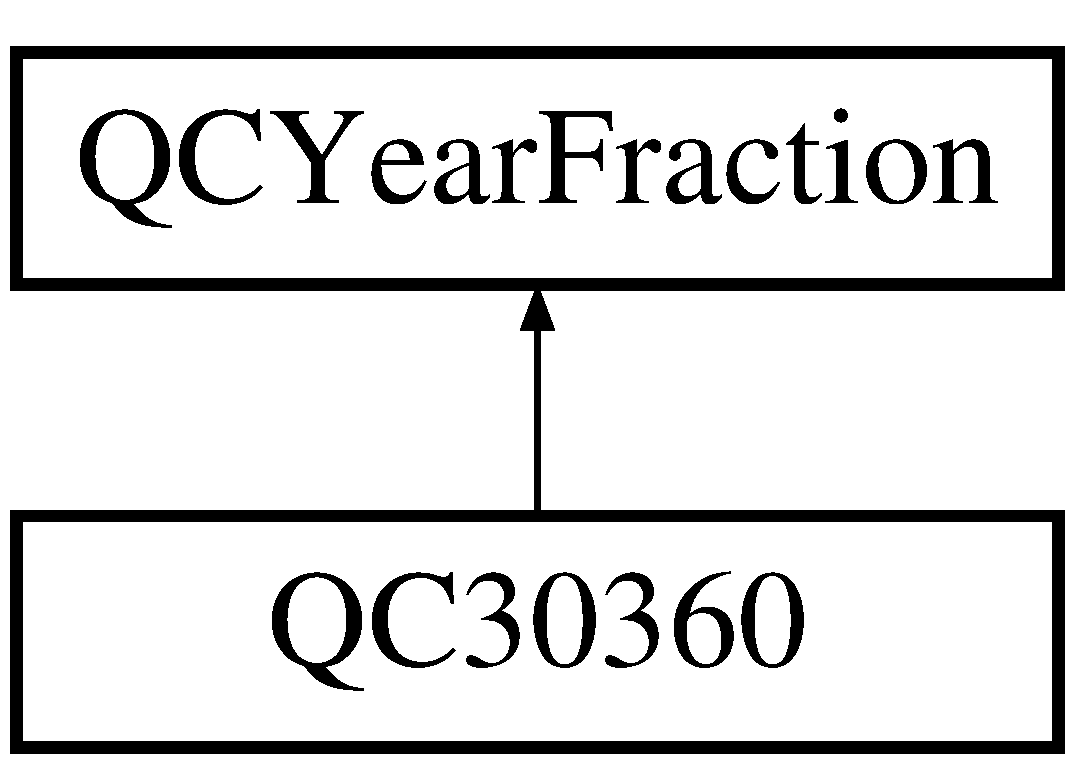
\includegraphics[height=2.000000cm]{class_q_c30360}
\end{center}
\end{figure}
\subsection*{Public Member Functions}
\begin{DoxyCompactItemize}
\item 
double \hyperlink{class_q_c30360_a4db09c9e51398c7b1bf99059d2d83094}{yf} (const \hyperlink{class_q_c_date}{Q\+C\+Date} \&first\+Date, const \hyperlink{class_q_c_date}{Q\+C\+Date} \&second\+Date)
\item 
long \hyperlink{class_q_c30360_a84ce06c39d386055dc91e43602e4d9e7}{count\+Days} (const \hyperlink{class_q_c_date}{Q\+C\+Date} \&first\+Date, const \hyperlink{class_q_c_date}{Q\+C\+Date} \&second\+Date)
\item 
virtual double \hyperlink{class_q_c30360_a9e7776fc765df31d5b60e8f7f87d4d55}{yf} (long days)
\end{DoxyCompactItemize}


\subsection{Detailed Description}
La clase \hyperlink{class_q_c30360}{Q\+C30360} implementa el método 30/360. Hereda de la clase abstracta \hyperlink{class_q_c_year_fraction}{Q\+C\+Year\+Fraction}. 

\begin{DoxyAuthor}{Author}
Alvaro Díaz 
\end{DoxyAuthor}


Definition at line 17 of file Q\+C30360.\+h.



\subsection{Member Function Documentation}
\hypertarget{class_q_c30360_a84ce06c39d386055dc91e43602e4d9e7}{\index{Q\+C30360@{Q\+C30360}!count\+Days@{count\+Days}}
\index{count\+Days@{count\+Days}!Q\+C30360@{Q\+C30360}}
\subsubsection[{count\+Days}]{\setlength{\rightskip}{0pt plus 5cm}long Q\+C30360\+::count\+Days (
\begin{DoxyParamCaption}
\item[{const {\bf Q\+C\+Date} \&}]{first\+Date, }
\item[{const {\bf Q\+C\+Date} \&}]{second\+Date}
\end{DoxyParamCaption}
)\hspace{0.3cm}{\ttfamily [virtual]}}}\label{class_q_c30360_a84ce06c39d386055dc91e43602e4d9e7}
La función count\+Days devuelve el número de días entre first\+Date y second\+Date en 30/360. Si se desea un número positivo first\+Date debe ser menor que second\+Date 
\begin{DoxyParams}{Parameters}
{\em first\+Date} & es la fecha más antigua de las dos si se desea retornar un valor positivo \\
\hline
{\em second\+Date} & es la fecha más reciente de las dos si se desea retornar un valor positivo \\
\hline
\end{DoxyParams}
\begin{DoxyReturn}{Returns}
un long con el número de días calculados 
\end{DoxyReturn}


Reimplemented from \hyperlink{class_q_c_year_fraction_aca9bd1b20d467d0a516bd19f0ef680e7}{Q\+C\+Year\+Fraction}.

\hypertarget{class_q_c30360_a4db09c9e51398c7b1bf99059d2d83094}{\index{Q\+C30360@{Q\+C30360}!yf@{yf}}
\index{yf@{yf}!Q\+C30360@{Q\+C30360}}
\subsubsection[{yf}]{\setlength{\rightskip}{0pt plus 5cm}double Q\+C30360\+::yf (
\begin{DoxyParamCaption}
\item[{const {\bf Q\+C\+Date} \&}]{first\+Date, }
\item[{const {\bf Q\+C\+Date} \&}]{second\+Date}
\end{DoxyParamCaption}
)\hspace{0.3cm}{\ttfamily [virtual]}}}\label{class_q_c30360_a4db09c9e51398c7b1bf99059d2d83094}
La función yf devuelve la fracción de año entre dos fechas en convención 30/360. 
\begin{DoxyParams}{Parameters}
{\em first\+Date} & es la fecha más antigua de las dos si se desea retornar un valor positivo \\
\hline
{\em second\+Date} & es la fecha más reciente de las dos si se desea retornar un valor positivo \\
\hline
\end{DoxyParams}
\begin{DoxyReturn}{Returns}
un double con la fracción de año calculada 
\end{DoxyReturn}


Reimplemented from \hyperlink{class_q_c_year_fraction_abf6d0f4b18d13ce6d31104332511c200}{Q\+C\+Year\+Fraction}.

\hypertarget{class_q_c30360_a9e7776fc765df31d5b60e8f7f87d4d55}{\index{Q\+C30360@{Q\+C30360}!yf@{yf}}
\index{yf@{yf}!Q\+C30360@{Q\+C30360}}
\subsubsection[{yf}]{\setlength{\rightskip}{0pt plus 5cm}virtual double Q\+C30360\+::yf (
\begin{DoxyParamCaption}
\item[{long}]{days}
\end{DoxyParamCaption}
)\hspace{0.3cm}{\ttfamily [virtual]}}}\label{class_q_c30360_a9e7776fc765df31d5b60e8f7f87d4d55}
La función yf devuelve un proxy de la fracción de año cuando el argumento es un numero de dias. 
\begin{DoxyParams}{Parameters}
{\em days} & corresponde a un numero de dias suponiendo que este numero ya esta bien calculado \\
\hline
\end{DoxyParams}
\begin{DoxyReturn}{Returns}
un double con la fracción de año calculada 
\end{DoxyReturn}


Reimplemented from \hyperlink{class_q_c_year_fraction_ac8ae7d0408e01f1e58d8ab6afe1ced3f}{Q\+C\+Year\+Fraction}.



The documentation for this class was generated from the following file\+:\begin{DoxyCompactItemize}
\item 
include/Q\+C30360.\+h\end{DoxyCompactItemize}

\hypertarget{class_q_c_act360}{\section{Q\+C\+Act360 Class Reference}
\label{class_q_c_act360}\index{Q\+C\+Act360@{Q\+C\+Act360}}
}


La clase \hyperlink{class_q_c_act360}{Q\+C\+Act360} implementa el método Act/360. Hereda de la clase abstracta \hyperlink{class_q_c_year_fraction}{Q\+C\+Year\+Fraction}.  




{\ttfamily \#include $<$Q\+C\+Act360.\+h$>$}

Inheritance diagram for Q\+C\+Act360\+:\begin{figure}[H]
\begin{center}
\leavevmode
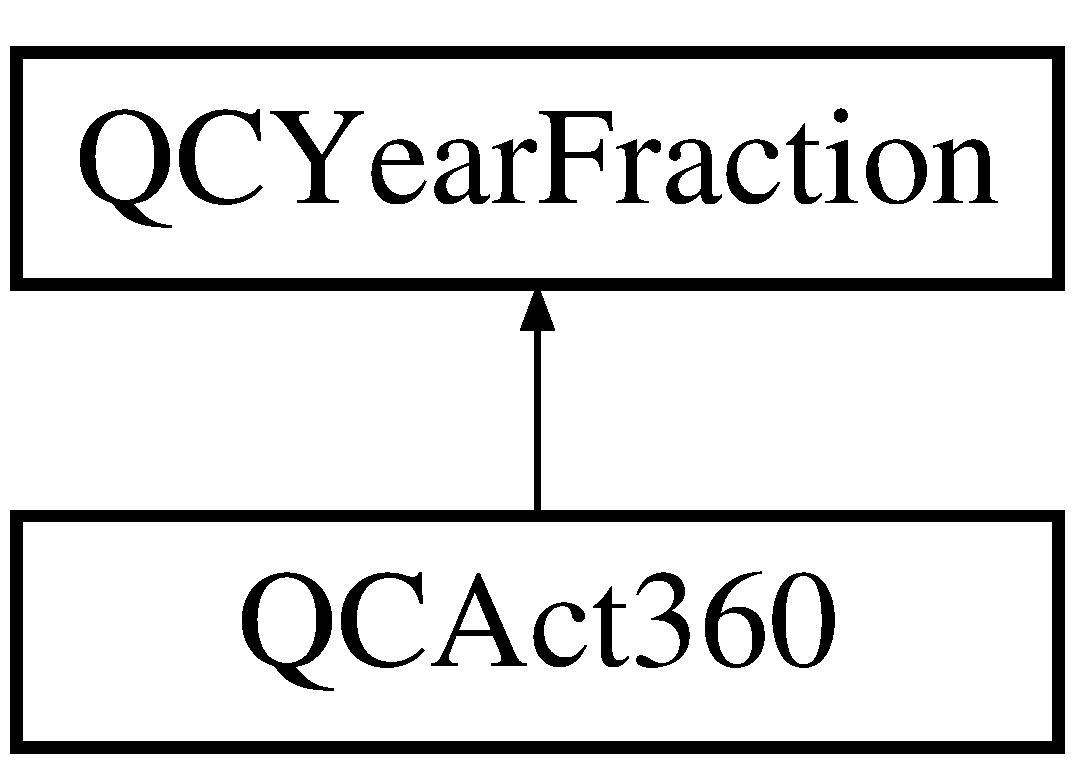
\includegraphics[height=2.000000cm]{class_q_c_act360}
\end{center}
\end{figure}
\subsection*{Public Member Functions}
\begin{DoxyCompactItemize}
\item 
double \hyperlink{class_q_c_act360_a63b8c11fddd7949ad0cfa2280ca229e9}{yf} (const \hyperlink{class_q_c_date}{Q\+C\+Date} \&first\+Date, const \hyperlink{class_q_c_date}{Q\+C\+Date} \&second\+Date)
\item 
virtual double \hyperlink{class_q_c_act360_a103e41364093ca0d0157d5782b88dec4}{yf} (long days)
\item 
long \hyperlink{class_q_c_act360_a415e4b5c9d5b5e5b1b9a3fd52795016b}{count\+Days} (const \hyperlink{class_q_c_date}{Q\+C\+Date} \&first\+Date, const \hyperlink{class_q_c_date}{Q\+C\+Date} \&second\+Date)
\end{DoxyCompactItemize}


\subsection{Detailed Description}
La clase \hyperlink{class_q_c_act360}{Q\+C\+Act360} implementa el método Act/360. Hereda de la clase abstracta \hyperlink{class_q_c_year_fraction}{Q\+C\+Year\+Fraction}. 

Definition at line 15 of file Q\+C\+Act360.\+h.



\subsection{Member Function Documentation}
\hypertarget{class_q_c_act360_a415e4b5c9d5b5e5b1b9a3fd52795016b}{\index{Q\+C\+Act360@{Q\+C\+Act360}!count\+Days@{count\+Days}}
\index{count\+Days@{count\+Days}!Q\+C\+Act360@{Q\+C\+Act360}}
\subsubsection[{count\+Days}]{\setlength{\rightskip}{0pt plus 5cm}long Q\+C\+Act360\+::count\+Days (
\begin{DoxyParamCaption}
\item[{const {\bf Q\+C\+Date} \&}]{first\+Date, }
\item[{const {\bf Q\+C\+Date} \&}]{second\+Date}
\end{DoxyParamCaption}
)\hspace{0.3cm}{\ttfamily [virtual]}}}\label{class_q_c_act360_a415e4b5c9d5b5e5b1b9a3fd52795016b}
La función count\+Days devuelve el número de días entre first\+Date y second\+Date en Act/360. Si se desea un número positivo first\+Date debe ser menor que second\+Date 
\begin{DoxyParams}[1]{Parameters}
\mbox{\tt in}  & {\em first\+Date} & es la fecha más antigua de las dos si se desea retornar un valor positivo \\
\hline
\mbox{\tt in}  & {\em second\+Date} & es la fecha más reciente de las dos si se desea retornar un valor positivo \\
\hline
\end{DoxyParams}
\begin{DoxyReturn}{Returns}
un long con el número de días calculados 
\end{DoxyReturn}


Reimplemented from \hyperlink{class_q_c_year_fraction_aca9bd1b20d467d0a516bd19f0ef680e7}{Q\+C\+Year\+Fraction}.

\hypertarget{class_q_c_act360_a63b8c11fddd7949ad0cfa2280ca229e9}{\index{Q\+C\+Act360@{Q\+C\+Act360}!yf@{yf}}
\index{yf@{yf}!Q\+C\+Act360@{Q\+C\+Act360}}
\subsubsection[{yf}]{\setlength{\rightskip}{0pt plus 5cm}double Q\+C\+Act360\+::yf (
\begin{DoxyParamCaption}
\item[{const {\bf Q\+C\+Date} \&}]{first\+Date, }
\item[{const {\bf Q\+C\+Date} \&}]{second\+Date}
\end{DoxyParamCaption}
)\hspace{0.3cm}{\ttfamily [virtual]}}}\label{class_q_c_act360_a63b8c11fddd7949ad0cfa2280ca229e9}
La función yf devuelve la fracción de año entre dos fechas en convención Act/360. 
\begin{DoxyParams}[1]{Parameters}
\mbox{\tt in}  & {\em first\+Date} & es la fecha más antigua de las dos si se desea retornar un valor positivo \\
\hline
\mbox{\tt in}  & {\em second\+Date} & es la fecha más reciente de las dos si se desea retornar un valor positivo \\
\hline
\end{DoxyParams}
\begin{DoxyReturn}{Returns}
un double con la fracción de año calculada 
\end{DoxyReturn}


Reimplemented from \hyperlink{class_q_c_year_fraction_abf6d0f4b18d13ce6d31104332511c200}{Q\+C\+Year\+Fraction}.

\hypertarget{class_q_c_act360_a103e41364093ca0d0157d5782b88dec4}{\index{Q\+C\+Act360@{Q\+C\+Act360}!yf@{yf}}
\index{yf@{yf}!Q\+C\+Act360@{Q\+C\+Act360}}
\subsubsection[{yf}]{\setlength{\rightskip}{0pt plus 5cm}virtual double Q\+C\+Act360\+::yf (
\begin{DoxyParamCaption}
\item[{long}]{days}
\end{DoxyParamCaption}
)\hspace{0.3cm}{\ttfamily [virtual]}}}\label{class_q_c_act360_a103e41364093ca0d0157d5782b88dec4}
La función yf devuelve un proxy de la fracción de año cuando el argumento es un numero de dias. 
\begin{DoxyParams}{Parameters}
{\em days} & \\
\hline
\end{DoxyParams}
\begin{DoxyReturn}{Returns}
un double con la fracción de año calculada 
\end{DoxyReturn}


Reimplemented from \hyperlink{class_q_c_year_fraction_ac8ae7d0408e01f1e58d8ab6afe1ced3f}{Q\+C\+Year\+Fraction}.



The documentation for this class was generated from the following file\+:\begin{DoxyCompactItemize}
\item 
include/Q\+C\+Act360.\+h\end{DoxyCompactItemize}

\hypertarget{class_q_c_act365}{\section{Q\+C\+Act365 Class Reference}
\label{class_q_c_act365}\index{Q\+C\+Act365@{Q\+C\+Act365}}
}


La clase \hyperlink{class_q_c_act360}{Q\+C\+Act360} implementa el método Act/365. Hereda de la clase abstracta \hyperlink{class_q_c_year_fraction}{Q\+C\+Year\+Fraction}.  




{\ttfamily \#include $<$Q\+C\+Act365.\+h$>$}

Inheritance diagram for Q\+C\+Act365\+:\begin{figure}[H]
\begin{center}
\leavevmode
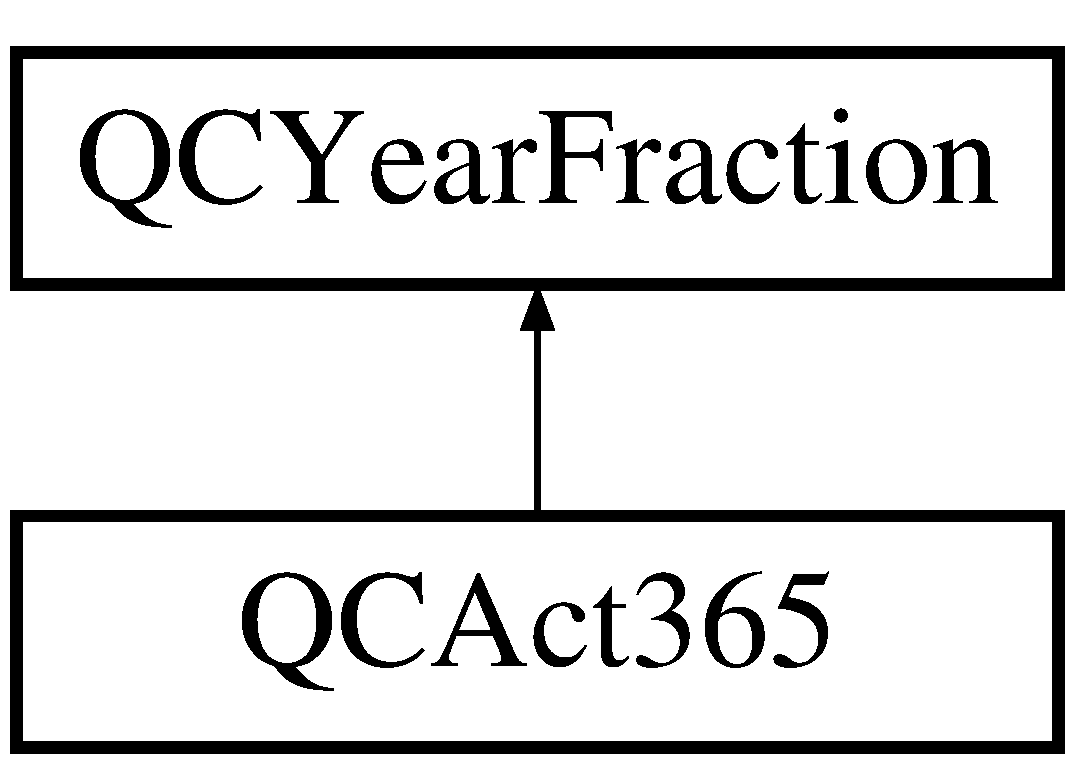
\includegraphics[height=2.000000cm]{class_q_c_act365}
\end{center}
\end{figure}
\subsection*{Public Member Functions}
\begin{DoxyCompactItemize}
\item 
double \hyperlink{class_q_c_act365_ae9ef9155b65718a4e7af7c706c576d95}{yf} (const \hyperlink{class_q_c_date}{Q\+C\+Date} \&first\+Date, const \hyperlink{class_q_c_date}{Q\+C\+Date} \&second\+Date)
\item 
virtual double \hyperlink{class_q_c_act365_a9579bfd75fece5fbd5391a57348f6d1e}{yf} (long days)
\item 
long \hyperlink{class_q_c_act365_a56509add10cf3573bd568390d1035d0b}{count\+Days} (const \hyperlink{class_q_c_date}{Q\+C\+Date} \&first\+Date, const \hyperlink{class_q_c_date}{Q\+C\+Date} \&second\+Date)
\end{DoxyCompactItemize}


\subsection{Detailed Description}
La clase \hyperlink{class_q_c_act360}{Q\+C\+Act360} implementa el método Act/365. Hereda de la clase abstracta \hyperlink{class_q_c_year_fraction}{Q\+C\+Year\+Fraction}. 

Definition at line 15 of file Q\+C\+Act365.\+h.



\subsection{Member Function Documentation}
\hypertarget{class_q_c_act365_a56509add10cf3573bd568390d1035d0b}{\index{Q\+C\+Act365@{Q\+C\+Act365}!count\+Days@{count\+Days}}
\index{count\+Days@{count\+Days}!Q\+C\+Act365@{Q\+C\+Act365}}
\subsubsection[{count\+Days}]{\setlength{\rightskip}{0pt plus 5cm}long Q\+C\+Act365\+::count\+Days (
\begin{DoxyParamCaption}
\item[{const {\bf Q\+C\+Date} \&}]{first\+Date, }
\item[{const {\bf Q\+C\+Date} \&}]{second\+Date}
\end{DoxyParamCaption}
)\hspace{0.3cm}{\ttfamily [virtual]}}}\label{class_q_c_act365_a56509add10cf3573bd568390d1035d0b}
La función count\+Days devuelve el número de días entre first\+Date y second\+Date en Act/365. Si se desea un número positivo first\+Date debe ser menor que second\+Date 
\begin{DoxyParams}[1]{Parameters}
\mbox{\tt in}  & {\em first\+Date} & es la fecha más antigua de las dos si se desea retornar un valor positivo \\
\hline
\mbox{\tt in}  & {\em second\+Date} & es la fecha más reciente de las dos si se desea retornar un valor positivo \\
\hline
\end{DoxyParams}
\begin{DoxyReturn}{Returns}
un long con el número de días calculados 
\end{DoxyReturn}


Reimplemented from \hyperlink{class_q_c_year_fraction_aca9bd1b20d467d0a516bd19f0ef680e7}{Q\+C\+Year\+Fraction}.

\hypertarget{class_q_c_act365_ae9ef9155b65718a4e7af7c706c576d95}{\index{Q\+C\+Act365@{Q\+C\+Act365}!yf@{yf}}
\index{yf@{yf}!Q\+C\+Act365@{Q\+C\+Act365}}
\subsubsection[{yf}]{\setlength{\rightskip}{0pt plus 5cm}double Q\+C\+Act365\+::yf (
\begin{DoxyParamCaption}
\item[{const {\bf Q\+C\+Date} \&}]{first\+Date, }
\item[{const {\bf Q\+C\+Date} \&}]{second\+Date}
\end{DoxyParamCaption}
)\hspace{0.3cm}{\ttfamily [virtual]}}}\label{class_q_c_act365_ae9ef9155b65718a4e7af7c706c576d95}
La función yf devuelve la fracción de año entre dos fechas en convención Act/365. 
\begin{DoxyParams}[1]{Parameters}
\mbox{\tt in}  & {\em first\+Date} & es la fecha más antigua de las dos si se desea retornar un valor positivo \\
\hline
\mbox{\tt in}  & {\em second\+Date} & es la fecha más reciente de las dos si se desea retornar un valor positivo \\
\hline
\end{DoxyParams}
\begin{DoxyReturn}{Returns}
un double con la fracción de año calculada 
\end{DoxyReturn}


Reimplemented from \hyperlink{class_q_c_year_fraction_abf6d0f4b18d13ce6d31104332511c200}{Q\+C\+Year\+Fraction}.

\hypertarget{class_q_c_act365_a9579bfd75fece5fbd5391a57348f6d1e}{\index{Q\+C\+Act365@{Q\+C\+Act365}!yf@{yf}}
\index{yf@{yf}!Q\+C\+Act365@{Q\+C\+Act365}}
\subsubsection[{yf}]{\setlength{\rightskip}{0pt plus 5cm}virtual double Q\+C\+Act365\+::yf (
\begin{DoxyParamCaption}
\item[{long}]{days}
\end{DoxyParamCaption}
)\hspace{0.3cm}{\ttfamily [virtual]}}}\label{class_q_c_act365_a9579bfd75fece5fbd5391a57348f6d1e}
La función yf devuelve un proxy de la fracción de año cuando el argumento es un numero de dias. 
\begin{DoxyParams}{Parameters}
{\em days} & \\
\hline
\end{DoxyParams}
\begin{DoxyReturn}{Returns}
un double con la fracción de año calculada 
\end{DoxyReturn}


Reimplemented from \hyperlink{class_q_c_year_fraction_ac8ae7d0408e01f1e58d8ab6afe1ced3f}{Q\+C\+Year\+Fraction}.



The documentation for this class was generated from the following file\+:\begin{DoxyCompactItemize}
\item 
include/Q\+C\+Act365.\+h\end{DoxyCompactItemize}

\hypertarget{class_q_c_act_act}{\section{Q\+C\+Act\+Act Class Reference}
\label{class_q_c_act_act}\index{Q\+C\+Act\+Act@{Q\+C\+Act\+Act}}
}


La clase \hyperlink{class_q_c_act360}{Q\+C\+Act360} implementa el método Act/\+Act. Hereda de la clase abstracta \hyperlink{class_q_c_year_fraction}{Q\+C\+Year\+Fraction}.  




{\ttfamily \#include $<$Q\+C\+Act\+Act.\+h$>$}

Inheritance diagram for Q\+C\+Act\+Act\+:\begin{figure}[H]
\begin{center}
\leavevmode
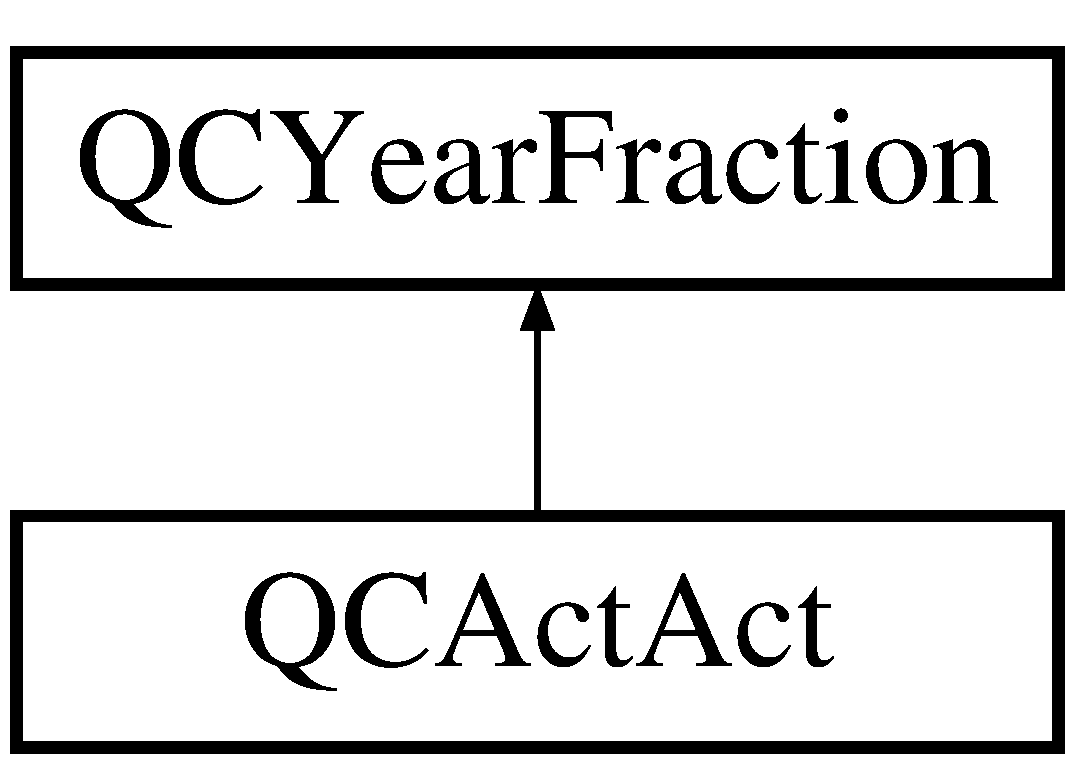
\includegraphics[height=2.000000cm]{class_q_c_act_act}
\end{center}
\end{figure}
\subsection*{Public Member Functions}
\begin{DoxyCompactItemize}
\item 
double \hyperlink{class_q_c_act_act_aa939d5d44744ffca64e36e3e9d2600bd}{yf} (const \hyperlink{class_q_c_date}{Q\+C\+Date} \&first\+Date, const \hyperlink{class_q_c_date}{Q\+C\+Date} \&second\+Date)
\item 
virtual double \hyperlink{class_q_c_act_act_ad22ae23fc988e029b70ac05db37b30fc}{yf} (long days)
\item 
long \hyperlink{class_q_c_act_act_a8d6cc524bd04550d07e1dc1f143e53e7}{count\+Days} (const \hyperlink{class_q_c_date}{Q\+C\+Date} \&first\+Date, const \hyperlink{class_q_c_date}{Q\+C\+Date} \&second\+Date)
\end{DoxyCompactItemize}


\subsection{Detailed Description}
La clase \hyperlink{class_q_c_act360}{Q\+C\+Act360} implementa el método Act/\+Act. Hereda de la clase abstracta \hyperlink{class_q_c_year_fraction}{Q\+C\+Year\+Fraction}. 

Definition at line 16 of file Q\+C\+Act\+Act.\+h.



\subsection{Member Function Documentation}
\hypertarget{class_q_c_act_act_a8d6cc524bd04550d07e1dc1f143e53e7}{\index{Q\+C\+Act\+Act@{Q\+C\+Act\+Act}!count\+Days@{count\+Days}}
\index{count\+Days@{count\+Days}!Q\+C\+Act\+Act@{Q\+C\+Act\+Act}}
\subsubsection[{count\+Days}]{\setlength{\rightskip}{0pt plus 5cm}long Q\+C\+Act\+Act\+::count\+Days (
\begin{DoxyParamCaption}
\item[{const {\bf Q\+C\+Date} \&}]{first\+Date, }
\item[{const {\bf Q\+C\+Date} \&}]{second\+Date}
\end{DoxyParamCaption}
)\hspace{0.3cm}{\ttfamily [virtual]}}}\label{class_q_c_act_act_a8d6cc524bd04550d07e1dc1f143e53e7}
La función count\+Days devuelve el número de días entre first\+Date y second\+Date en Act/\+Act. Si se desea un número positivo first\+Date debe ser menor que second\+Date 
\begin{DoxyParams}[1]{Parameters}
\mbox{\tt in}  & {\em first\+Date} & es la fecha más antigua de las dos si se desea retornar un valor positivo \\
\hline
\mbox{\tt in}  & {\em second\+Date} & es la fecha más reciente de las dos si se desea retornar un valor positivo \\
\hline
\end{DoxyParams}
\begin{DoxyReturn}{Returns}
un long con el número de días calculados 
\end{DoxyReturn}


Reimplemented from \hyperlink{class_q_c_year_fraction_aca9bd1b20d467d0a516bd19f0ef680e7}{Q\+C\+Year\+Fraction}.

\hypertarget{class_q_c_act_act_aa939d5d44744ffca64e36e3e9d2600bd}{\index{Q\+C\+Act\+Act@{Q\+C\+Act\+Act}!yf@{yf}}
\index{yf@{yf}!Q\+C\+Act\+Act@{Q\+C\+Act\+Act}}
\subsubsection[{yf}]{\setlength{\rightskip}{0pt plus 5cm}double Q\+C\+Act\+Act\+::yf (
\begin{DoxyParamCaption}
\item[{const {\bf Q\+C\+Date} \&}]{first\+Date, }
\item[{const {\bf Q\+C\+Date} \&}]{second\+Date}
\end{DoxyParamCaption}
)\hspace{0.3cm}{\ttfamily [virtual]}}}\label{class_q_c_act_act_aa939d5d44744ffca64e36e3e9d2600bd}
La función yf devuelve la fracción de año entre dos fechas en convención Act/\+Act. 
\begin{DoxyParams}[1]{Parameters}
\mbox{\tt in}  & {\em first\+Date} & es la fecha más antigua de las dos si se desea retornar un valor positivo \\
\hline
\mbox{\tt in}  & {\em second\+Date} & es la fecha más reciente de las dos si se desea retornar un valor positivo \\
\hline
\end{DoxyParams}
\begin{DoxyReturn}{Returns}
un double con la fracción de año calculada 
\end{DoxyReturn}


Reimplemented from \hyperlink{class_q_c_year_fraction_abf6d0f4b18d13ce6d31104332511c200}{Q\+C\+Year\+Fraction}.

\hypertarget{class_q_c_act_act_ad22ae23fc988e029b70ac05db37b30fc}{\index{Q\+C\+Act\+Act@{Q\+C\+Act\+Act}!yf@{yf}}
\index{yf@{yf}!Q\+C\+Act\+Act@{Q\+C\+Act\+Act}}
\subsubsection[{yf}]{\setlength{\rightskip}{0pt plus 5cm}virtual double Q\+C\+Act\+Act\+::yf (
\begin{DoxyParamCaption}
\item[{long}]{days}
\end{DoxyParamCaption}
)\hspace{0.3cm}{\ttfamily [virtual]}}}\label{class_q_c_act_act_ad22ae23fc988e029b70ac05db37b30fc}
La función yf devuelve un proxy de la fracción de año cuando el argumento es un numero de dias. 
\begin{DoxyParams}{Parameters}
{\em days} & \\
\hline
\end{DoxyParams}
\begin{DoxyReturn}{Returns}
un double con la fracción de año calculada 
\end{DoxyReturn}


Reimplemented from \hyperlink{class_q_c_year_fraction_ac8ae7d0408e01f1e58d8ab6afe1ced3f}{Q\+C\+Year\+Fraction}.



The documentation for this class was generated from the following file\+:\begin{DoxyCompactItemize}
\item 
include/Q\+C\+Act\+Act.\+h\end{DoxyCompactItemize}

\hypertarget{class_q_c_business_calendar}{\section{Q\+C\+Business\+Calendar Class Reference}
\label{class_q_c_business_calendar}\index{Q\+C\+Business\+Calendar@{Q\+C\+Business\+Calendar}}
}


La clase \hyperlink{class_q_c_business_calendar}{Q\+C\+Business\+Calendar} representa días feriados de una jurisdicción.  




{\ttfamily \#include $<$Q\+C\+Business\+Calendar.\+h$>$}

\subsection*{Public Member Functions}
\begin{DoxyCompactItemize}
\item 
\hyperlink{class_q_c_business_calendar_a4460142026e84efab275be4712c366f8}{Q\+C\+Business\+Calendar} (\hyperlink{class_q_c_date}{Q\+C\+Date} \&start\+Date, int length)
\item 
void \hyperlink{class_q_c_business_calendar_ab72834f0e628a1f903bcb4a32c22f346}{add\+Holyday} (const \hyperlink{class_q_c_date}{Q\+C\+Date} \&holyday)
\item 
\hyperlink{class_q_c_date}{Q\+C\+Date} \hyperlink{class_q_c_business_calendar_a5608f57e89472291cfdea26685b6eea6}{next\+Business\+Day} (const \hyperlink{class_q_c_date}{Q\+C\+Date} \&fecha)
\item 
\hyperlink{class_q_c_date}{Q\+C\+Date} \hyperlink{class_q_c_business_calendar_a83697d6856882aff5d315884bcdd8ed8}{mod\+Next\+Business\+Day} (const \hyperlink{class_q_c_date}{Q\+C\+Date} \&fecha)
\item 
\hyperlink{class_q_c_date}{Q\+C\+Date} \hyperlink{class_q_c_business_calendar_a90b4ba160b7a61818da7eb1e76305c6d}{previous\+Business\+Day} (const \hyperlink{class_q_c_date}{Q\+C\+Date} \&fecha)
\item 
\hyperlink{class_q_c_date}{Q\+C\+Date} \hyperlink{class_q_c_business_calendar_a7d5760e3664caa8b963d340998551ac5}{shift} (const \hyperlink{class_q_c_date}{Q\+C\+Date} \&fecha, int n\+Days)
\end{DoxyCompactItemize}


\subsection{Detailed Description}
La clase \hyperlink{class_q_c_business_calendar}{Q\+C\+Business\+Calendar} representa días feriados de una jurisdicción. 

Definition at line 16 of file Q\+C\+Business\+Calendar.\+h.



\subsection{Constructor \& Destructor Documentation}
\hypertarget{class_q_c_business_calendar_a4460142026e84efab275be4712c366f8}{\index{Q\+C\+Business\+Calendar@{Q\+C\+Business\+Calendar}!Q\+C\+Business\+Calendar@{Q\+C\+Business\+Calendar}}
\index{Q\+C\+Business\+Calendar@{Q\+C\+Business\+Calendar}!Q\+C\+Business\+Calendar@{Q\+C\+Business\+Calendar}}
\subsubsection[{Q\+C\+Business\+Calendar}]{\setlength{\rightskip}{0pt plus 5cm}Q\+C\+Business\+Calendar\+::\+Q\+C\+Business\+Calendar (
\begin{DoxyParamCaption}
\item[{{\bf Q\+C\+Date} \&}]{start\+Date, }
\item[{int}]{length}
\end{DoxyParamCaption}
)}}\label{class_q_c_business_calendar_a4460142026e84efab275be4712c366f8}
Constructor 
\begin{DoxyParams}{Parameters}
{\em start\+Date} & (\hyperlink{class_q_c_date}{Q\+C\+Date}) fecha inicial del calendario \\
\hline
{\em length} & (int) largo en años del calendario \\
\hline
\end{DoxyParams}
\begin{DoxyReturn}{Returns}
objeto construido 
\end{DoxyReturn}


\subsection{Member Function Documentation}
\hypertarget{class_q_c_business_calendar_ab72834f0e628a1f903bcb4a32c22f346}{\index{Q\+C\+Business\+Calendar@{Q\+C\+Business\+Calendar}!add\+Holyday@{add\+Holyday}}
\index{add\+Holyday@{add\+Holyday}!Q\+C\+Business\+Calendar@{Q\+C\+Business\+Calendar}}
\subsubsection[{add\+Holyday}]{\setlength{\rightskip}{0pt plus 5cm}void Q\+C\+Business\+Calendar\+::add\+Holyday (
\begin{DoxyParamCaption}
\item[{const {\bf Q\+C\+Date} \&}]{holyday}
\end{DoxyParamCaption}
)}}\label{class_q_c_business_calendar_ab72834f0e628a1f903bcb4a32c22f346}
Agrega una fecha (\hyperlink{class_q_c_date}{Q\+C\+Date}) al calendario (que representa un feriado) 
\begin{DoxyParams}{Parameters}
{\em holyday} & (\hyperlink{class_q_c_date}{Q\+C\+Date}) el feriado a agregar \\
\hline
\end{DoxyParams}
\hypertarget{class_q_c_business_calendar_a83697d6856882aff5d315884bcdd8ed8}{\index{Q\+C\+Business\+Calendar@{Q\+C\+Business\+Calendar}!mod\+Next\+Business\+Day@{mod\+Next\+Business\+Day}}
\index{mod\+Next\+Business\+Day@{mod\+Next\+Business\+Day}!Q\+C\+Business\+Calendar@{Q\+C\+Business\+Calendar}}
\subsubsection[{mod\+Next\+Business\+Day}]{\setlength{\rightskip}{0pt plus 5cm}{\bf Q\+C\+Date} Q\+C\+Business\+Calendar\+::mod\+Next\+Business\+Day (
\begin{DoxyParamCaption}
\item[{const {\bf Q\+C\+Date} \&}]{fecha}
\end{DoxyParamCaption}
)}}\label{class_q_c_business_calendar_a83697d6856882aff5d315884bcdd8ed8}
Calcula el día hábil siguiente a la fecha ingresada en comvención modificada. Si el día hábil siguiente cambia de mes respecto a la fecha ingresada, entonces retorna el día hábil anterior. Si la fecha ingresada es hábil se retorna la misma fecha. 
\begin{DoxyParams}{Parameters}
{\em fecha} & (\hyperlink{class_q_c_date}{Q\+C\+Date}) fecha ingresada \\
\hline
\end{DoxyParams}
\begin{DoxyReturn}{Returns}
el día hábil siguiente 
\end{DoxyReturn}
\hypertarget{class_q_c_business_calendar_a5608f57e89472291cfdea26685b6eea6}{\index{Q\+C\+Business\+Calendar@{Q\+C\+Business\+Calendar}!next\+Business\+Day@{next\+Business\+Day}}
\index{next\+Business\+Day@{next\+Business\+Day}!Q\+C\+Business\+Calendar@{Q\+C\+Business\+Calendar}}
\subsubsection[{next\+Business\+Day}]{\setlength{\rightskip}{0pt plus 5cm}{\bf Q\+C\+Date} Q\+C\+Business\+Calendar\+::next\+Business\+Day (
\begin{DoxyParamCaption}
\item[{const {\bf Q\+C\+Date} \&}]{fecha}
\end{DoxyParamCaption}
)}}\label{class_q_c_business_calendar_a5608f57e89472291cfdea26685b6eea6}
Calcula el día hábil siguiente a la fecha que ingresa. Si la fecha que ingresa es hábil se mantiene igual. 
\begin{DoxyParams}{Parameters}
{\em fecha} & (\hyperlink{class_q_c_date}{Q\+C\+Date}) fecha que ingresa \\
\hline
\end{DoxyParams}
\begin{DoxyReturn}{Returns}
(\hyperlink{class_q_c_date}{Q\+C\+Date}) el día hábil siguiente 
\end{DoxyReturn}
\hypertarget{class_q_c_business_calendar_a90b4ba160b7a61818da7eb1e76305c6d}{\index{Q\+C\+Business\+Calendar@{Q\+C\+Business\+Calendar}!previous\+Business\+Day@{previous\+Business\+Day}}
\index{previous\+Business\+Day@{previous\+Business\+Day}!Q\+C\+Business\+Calendar@{Q\+C\+Business\+Calendar}}
\subsubsection[{previous\+Business\+Day}]{\setlength{\rightskip}{0pt plus 5cm}{\bf Q\+C\+Date} Q\+C\+Business\+Calendar\+::previous\+Business\+Day (
\begin{DoxyParamCaption}
\item[{const {\bf Q\+C\+Date} \&}]{fecha}
\end{DoxyParamCaption}
)}}\label{class_q_c_business_calendar_a90b4ba160b7a61818da7eb1e76305c6d}
Calcula el día hábil anterior a la fecha ingresada 
\begin{DoxyParams}{Parameters}
{\em fecha} & (\hyperlink{class_q_c_date}{Q\+C\+Date}) \\
\hline
\end{DoxyParams}
\begin{DoxyReturn}{Returns}

\end{DoxyReturn}
\hypertarget{class_q_c_business_calendar_a7d5760e3664caa8b963d340998551ac5}{\index{Q\+C\+Business\+Calendar@{Q\+C\+Business\+Calendar}!shift@{shift}}
\index{shift@{shift}!Q\+C\+Business\+Calendar@{Q\+C\+Business\+Calendar}}
\subsubsection[{shift}]{\setlength{\rightskip}{0pt plus 5cm}{\bf Q\+C\+Date} Q\+C\+Business\+Calendar\+::shift (
\begin{DoxyParamCaption}
\item[{const {\bf Q\+C\+Date} \&}]{fecha, }
\item[{int}]{n\+Days}
\end{DoxyParamCaption}
)}}\label{class_q_c_business_calendar_a7d5760e3664caa8b963d340998551ac5}
Mueve una fecha un número n\+Days de días. 
\begin{DoxyParams}{Parameters}
{\em fecha} & (\hyperlink{class_q_c_date}{Q\+C\+Date}) fecha que se debe mover \\
\hline
{\em n\+Days} & (int) número de días a mover (pos o neg) \\
\hline
\end{DoxyParams}
\begin{DoxyReturn}{Returns}
(\hyperlink{class_q_c_date}{Q\+C\+Date}) fecha movida 
\end{DoxyReturn}


The documentation for this class was generated from the following file\+:\begin{DoxyCompactItemize}
\item 
include/Q\+C\+Business\+Calendar.\+h\end{DoxyCompactItemize}

\hypertarget{class_q_c_clamped_spline}{\section{Q\+C\+Clamped\+Spline Class Reference}
\label{class_q_c_clamped_spline}\index{Q\+C\+Clamped\+Spline@{Q\+C\+Clamped\+Spline}}
}
Inheritance diagram for Q\+C\+Clamped\+Spline\+:\begin{figure}[H]
\begin{center}
\leavevmode
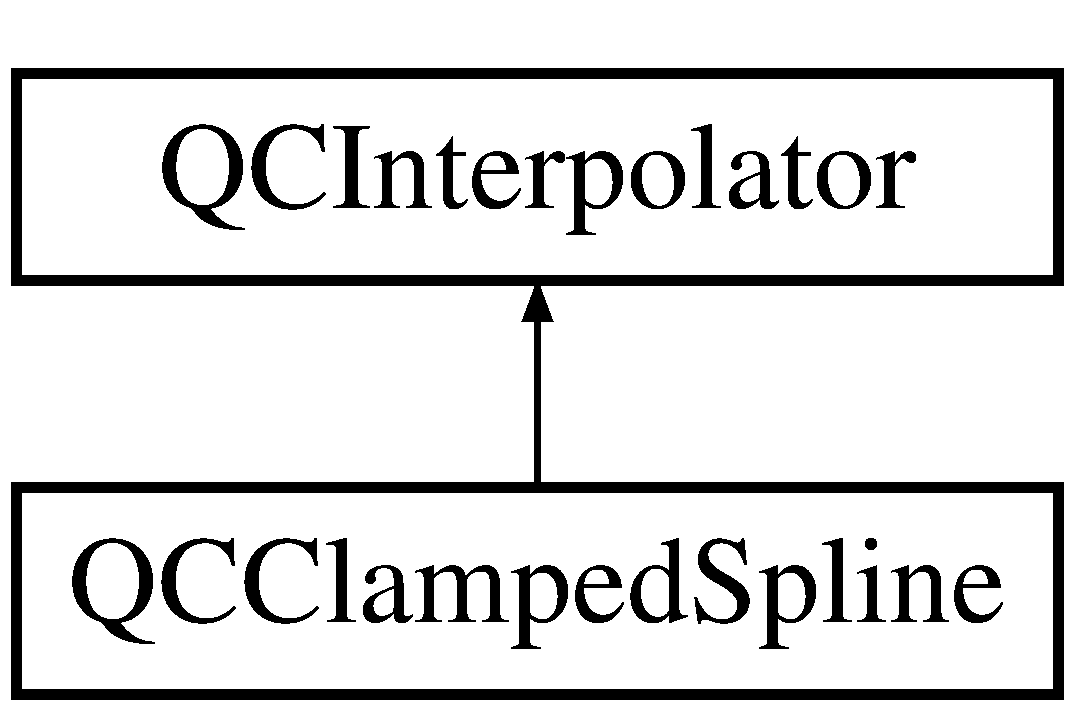
\includegraphics[height=2.000000cm]{class_q_c_clamped_spline}
\end{center}
\end{figure}
\subsection*{Public Member Functions}
\begin{DoxyCompactItemize}
\item 
\hypertarget{class_q_c_clamped_spline_af302b0106ede994e396db275f75fc4bf}{{\bfseries Q\+C\+Clamped\+Spline} (shared\+\_\+ptr$<$ \hyperlink{class_q_c_curve}{Q\+C\+Curve}$<$ long $>$$>$ curva)}\label{class_q_c_clamped_spline_af302b0106ede994e396db275f75fc4bf}

\item 
\hypertarget{class_q_c_clamped_spline_ad67f1624a00bd5760f9f086fe73805e6}{double {\bfseries interpolate\+At} (long value) override}\label{class_q_c_clamped_spline_ad67f1624a00bd5760f9f086fe73805e6}

\item 
\hypertarget{class_q_c_clamped_spline_ade6fba8584adad22700f464f84537fd6}{double {\bfseries derivative\+At} (long value) override}\label{class_q_c_clamped_spline_ade6fba8584adad22700f464f84537fd6}

\item 
\hypertarget{class_q_c_clamped_spline_a5ed512afe79288b3efd56690a2201380}{double {\bfseries second\+Derivative\+At} (long value) override}\label{class_q_c_clamped_spline_a5ed512afe79288b3efd56690a2201380}

\end{DoxyCompactItemize}
\subsection*{Additional Inherited Members}


\subsection{Detailed Description}


Definition at line 7 of file Q\+C\+Clamped\+Spline.\+h.



The documentation for this class was generated from the following file\+:\begin{DoxyCompactItemize}
\item 
include/Q\+C\+Clamped\+Spline.\+h\end{DoxyCompactItemize}

\hypertarget{class_q_c_compound_wf}{\section{Q\+C\+Compound\+Wf Class Reference}
\label{class_q_c_compound_wf}\index{Q\+C\+Compound\+Wf@{Q\+C\+Compound\+Wf}}
}
Inheritance diagram for Q\+C\+Compound\+Wf\+:\begin{figure}[H]
\begin{center}
\leavevmode
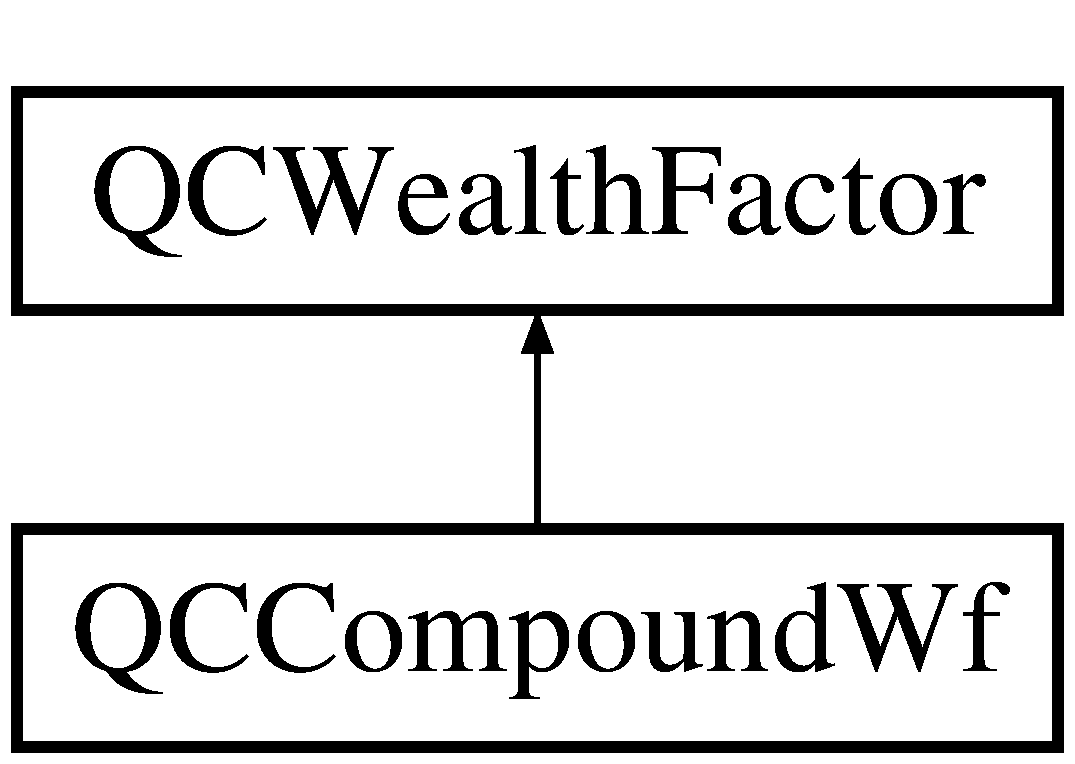
\includegraphics[height=2.000000cm]{class_q_c_compound_wf}
\end{center}
\end{figure}
\subsection*{Public Member Functions}
\begin{DoxyCompactItemize}
\item 
virtual double \hyperlink{class_q_c_compound_wf_a96e3c92f84af47a241a4e24ad470536a}{wf} (double \hyperlink{class_q_c_compound_wf_a49832a3141f59a281e1ccc8396724bb8}{rate}, double yf) override
\item 
virtual double \hyperlink{class_q_c_compound_wf_a49832a3141f59a281e1ccc8396724bb8}{rate} (double \hyperlink{class_q_c_compound_wf_a96e3c92f84af47a241a4e24ad470536a}{wf}, double yf) override
\end{DoxyCompactItemize}
\subsection*{Additional Inherited Members}


\subsection{Detailed Description}


Definition at line 5 of file Q\+C\+Compound\+Wf.\+h.



\subsection{Member Function Documentation}
\hypertarget{class_q_c_compound_wf_a49832a3141f59a281e1ccc8396724bb8}{\index{Q\+C\+Compound\+Wf@{Q\+C\+Compound\+Wf}!rate@{rate}}
\index{rate@{rate}!Q\+C\+Compound\+Wf@{Q\+C\+Compound\+Wf}}
\subsubsection[{rate}]{\setlength{\rightskip}{0pt plus 5cm}virtual double Q\+C\+Compound\+Wf\+::rate (
\begin{DoxyParamCaption}
\item[{double}]{wf, }
\item[{double}]{yf}
\end{DoxyParamCaption}
)\hspace{0.3cm}{\ttfamily [override]}, {\ttfamily [virtual]}}}\label{class_q_c_compound_wf_a49832a3141f59a281e1ccc8396724bb8}
La función rate devuelve el valor de la tasa asociada al valor del factor de capitalización y su fracción de año asociada. 
\begin{DoxyParams}{Parameters}
{\em wf} & es el valor del factor de capitalización \\
\hline
{\em yf} & es el valor de la fracción de año \\
\hline
\end{DoxyParams}
\begin{DoxyReturn}{Returns}
(double) valor de la tasa asociada 
\end{DoxyReturn}


Implements \hyperlink{class_q_c_wealth_factor_aad4a3d84f0c2073162cc5fcce5509d1c}{Q\+C\+Wealth\+Factor}.

\hypertarget{class_q_c_compound_wf_a96e3c92f84af47a241a4e24ad470536a}{\index{Q\+C\+Compound\+Wf@{Q\+C\+Compound\+Wf}!wf@{wf}}
\index{wf@{wf}!Q\+C\+Compound\+Wf@{Q\+C\+Compound\+Wf}}
\subsubsection[{wf}]{\setlength{\rightskip}{0pt plus 5cm}virtual double Q\+C\+Compound\+Wf\+::wf (
\begin{DoxyParamCaption}
\item[{double}]{rate, }
\item[{double}]{yf}
\end{DoxyParamCaption}
)\hspace{0.3cm}{\ttfamily [override]}, {\ttfamily [virtual]}}}\label{class_q_c_compound_wf_a96e3c92f84af47a241a4e24ad470536a}
La función wf devuelve el valor del factor de capitalización dado el valor de una tasa y su fracción de año asociada. Cuando se invoca este método, también se calcula la derivada del factor de capitalización respecto al parámetro rate. Este valor se almacena en la variable protected \+\_\+dwf 
\begin{DoxyParams}{Parameters}
{\em rate} & es el valor de la tasa \\
\hline
{\em yf} & es el valor de la fracción de año \\
\hline
\end{DoxyParams}
\begin{DoxyReturn}{Returns}
(double) valor del factor de capitalización 
\end{DoxyReturn}


Implements \hyperlink{class_q_c_wealth_factor_a63ddc9c957aa438c1278b541f6e1ebbe}{Q\+C\+Wealth\+Factor}.



The documentation for this class was generated from the following file\+:\begin{DoxyCompactItemize}
\item 
include/Q\+C\+Compound\+Wf.\+h\end{DoxyCompactItemize}

\hypertarget{class_q_c_continous_wf}{\section{Q\+C\+Continous\+Wf Class Reference}
\label{class_q_c_continous_wf}\index{Q\+C\+Continous\+Wf@{Q\+C\+Continous\+Wf}}
}
Inheritance diagram for Q\+C\+Continous\+Wf\+:\begin{figure}[H]
\begin{center}
\leavevmode
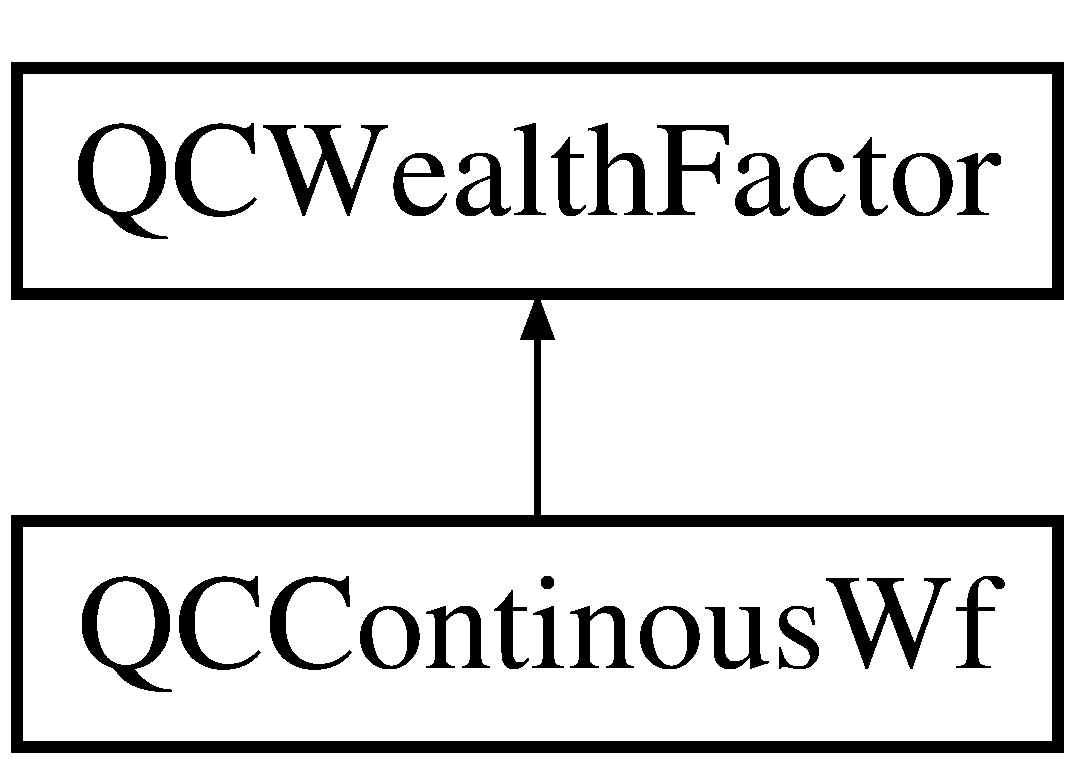
\includegraphics[height=2.000000cm]{class_q_c_continous_wf}
\end{center}
\end{figure}
\subsection*{Public Member Functions}
\begin{DoxyCompactItemize}
\item 
virtual double \hyperlink{class_q_c_continous_wf_a0384d407c9dc90c1579b0ba53d881d5d}{wf} (double \hyperlink{class_q_c_continous_wf_addd920e12675b08c941c791e09ceca4a}{rate}, double yf) override
\item 
virtual double \hyperlink{class_q_c_continous_wf_addd920e12675b08c941c791e09ceca4a}{rate} (double \hyperlink{class_q_c_continous_wf_a0384d407c9dc90c1579b0ba53d881d5d}{wf}, double yf) override
\end{DoxyCompactItemize}
\subsection*{Additional Inherited Members}


\subsection{Detailed Description}


Definition at line 5 of file Q\+C\+Continous\+Wf.\+h.



\subsection{Member Function Documentation}
\hypertarget{class_q_c_continous_wf_addd920e12675b08c941c791e09ceca4a}{\index{Q\+C\+Continous\+Wf@{Q\+C\+Continous\+Wf}!rate@{rate}}
\index{rate@{rate}!Q\+C\+Continous\+Wf@{Q\+C\+Continous\+Wf}}
\subsubsection[{rate}]{\setlength{\rightskip}{0pt plus 5cm}virtual double Q\+C\+Continous\+Wf\+::rate (
\begin{DoxyParamCaption}
\item[{double}]{wf, }
\item[{double}]{yf}
\end{DoxyParamCaption}
)\hspace{0.3cm}{\ttfamily [override]}, {\ttfamily [virtual]}}}\label{class_q_c_continous_wf_addd920e12675b08c941c791e09ceca4a}
La función rate devuelve el valor de la tasa asociada al valor del factor de capitalización y su fracción de año asociada. 
\begin{DoxyParams}{Parameters}
{\em wf} & es el valor del factor de capitalización \\
\hline
{\em yf} & es el valor de la fracción de año \\
\hline
\end{DoxyParams}
\begin{DoxyReturn}{Returns}
(double) valor de la tasa asociada 
\end{DoxyReturn}


Implements \hyperlink{class_q_c_wealth_factor_aad4a3d84f0c2073162cc5fcce5509d1c}{Q\+C\+Wealth\+Factor}.

\hypertarget{class_q_c_continous_wf_a0384d407c9dc90c1579b0ba53d881d5d}{\index{Q\+C\+Continous\+Wf@{Q\+C\+Continous\+Wf}!wf@{wf}}
\index{wf@{wf}!Q\+C\+Continous\+Wf@{Q\+C\+Continous\+Wf}}
\subsubsection[{wf}]{\setlength{\rightskip}{0pt plus 5cm}virtual double Q\+C\+Continous\+Wf\+::wf (
\begin{DoxyParamCaption}
\item[{double}]{rate, }
\item[{double}]{yf}
\end{DoxyParamCaption}
)\hspace{0.3cm}{\ttfamily [override]}, {\ttfamily [virtual]}}}\label{class_q_c_continous_wf_a0384d407c9dc90c1579b0ba53d881d5d}
La función wf devuelve el valor del factor de capitalización dado el valor de una tasa y su fracción de año asociada. Cuando se invoca este método, también se calcula la derivada del factor de capitalización respecto al parámetro rate. Este valor se almacena en la variable protected \+\_\+dwf 
\begin{DoxyParams}{Parameters}
{\em rate} & es el valor de la tasa \\
\hline
{\em yf} & es el valor de la fracción de año \\
\hline
\end{DoxyParams}
\begin{DoxyReturn}{Returns}
(double) valor del factor de capitalización 
\end{DoxyReturn}


Implements \hyperlink{class_q_c_wealth_factor_a63ddc9c957aa438c1278b541f6e1ebbe}{Q\+C\+Wealth\+Factor}.



The documentation for this class was generated from the following file\+:\begin{DoxyCompactItemize}
\item 
include/Q\+C\+Continous\+Wf.\+h\end{DoxyCompactItemize}

\hypertarget{class_q_c_curve}{\section{Q\+C\+Curve$<$ T $>$ Class Template Reference}
\label{class_q_c_curve}\index{Q\+C\+Curve$<$ T $>$@{Q\+C\+Curve$<$ T $>$}}
}
\subsection*{Public Member Functions}
\begin{DoxyCompactItemize}
\item 
\hypertarget{class_q_c_curve_ae06036e13e430dd4151357bd649c9253}{{\bfseries Q\+C\+Curve} (vector$<$ T $>$ \&abscissa, vector$<$ double $>$ \&ordinate)}\label{class_q_c_curve_ae06036e13e430dd4151357bd649c9253}

\item 
\hypertarget{class_q_c_curve_a6ee52258c32718dc9c6c566286a35511}{pair$<$ T, double $>$ {\bfseries get\+Values\+At} (long position)}\label{class_q_c_curve_a6ee52258c32718dc9c6c566286a35511}

\item 
\hypertarget{class_q_c_curve_a196e3a697e436a9f2ce30ff228580899}{long {\bfseries get\+Length} ()}\label{class_q_c_curve_a196e3a697e436a9f2ce30ff228580899}

\end{DoxyCompactItemize}
\subsection*{Protected Attributes}
\begin{DoxyCompactItemize}
\item 
\hypertarget{class_q_c_curve_af2bb246f5a1afba933bbada9d3a3c742}{vector$<$ pair$<$ T, double $>$ $>$ {\bfseries \+\_\+values}}\label{class_q_c_curve_af2bb246f5a1afba933bbada9d3a3c742}

\end{DoxyCompactItemize}


\subsection{Detailed Description}
\subsubsection*{template$<$class T$>$class Q\+C\+Curve$<$ T $>$}



Definition at line 12 of file Q\+C\+Curve.\+h.



The documentation for this class was generated from the following file\+:\begin{DoxyCompactItemize}
\item 
include/Q\+C\+Curve.\+h\end{DoxyCompactItemize}

\hypertarget{class_q_c_date}{\section{Q\+C\+Date Class Reference}
\label{class_q_c_date}\index{Q\+C\+Date@{Q\+C\+Date}}
}


\hyperlink{class_q_c_date}{Q\+C\+Date} es la implementación de Q\+Code de una clase para manejar fechas.  




{\ttfamily \#include $<$Q\+C\+Date.\+h$>$}

\subsection*{Public Types}
\begin{DoxyCompactItemize}
\item 
enum \hyperlink{class_q_c_date_a19bc952d3dba68ce61881ec85837c7eb}{Q\+C\+Week\+Day} \{ \\*
{\bfseries qc\+Monday} = 1, 
{\bfseries qc\+Tuesday} = 2, 
{\bfseries qc\+Wednesday} = 3, 
{\bfseries qc\+Thursday} = 4, 
\\*
{\bfseries qc\+Friday} = 5, 
{\bfseries qc\+Saturday} = 6, 
{\bfseries qc\+Sunday} = 0
 \}
\item 
enum \hyperlink{class_q_c_date_a17e5b6c9a1a784f917c8e84045d7e362}{Q\+C\+Bus\+Day\+Adj\+Rules} \{ \\*
{\bfseries qc\+No} = 0, 
{\bfseries qc\+Follow} = 1, 
{\bfseries qc\+Mod\+Follow} = 2, 
{\bfseries qc\+Prev} = 3, 
\\*
{\bfseries qc\+Mod\+Prev} = 4
 \}
\end{DoxyCompactItemize}
\subsection*{Public Member Functions}
\begin{DoxyCompactItemize}
\item 
\hyperlink{class_q_c_date_a4668aa0f8cc6671f1f4413a9d9152bce}{Q\+C\+Date} ()
\item 
\hyperlink{class_q_c_date_aa4234ef62a09004355f1a8c227bb0b80}{Q\+C\+Date} (long \hyperlink{class_q_c_date_a91dae9aacdc06dcc3c3aaac686a6a6f7}{excel\+Serial})
\item 
\hyperlink{class_q_c_date_a9f91ba907afd6cce87c9d1d114658ac4}{Q\+C\+Date} (int d, int m, int y)
\item 
\hyperlink{class_q_c_date_a8e41bf9b439d97d9abe4e9ee25f719a9}{Q\+C\+Date} (string \&string\+Date)
\item 
\hyperlink{class_q_c_date_af5f2687a03cda466dc5da09a60b88f69}{Q\+C\+Date} (const \hyperlink{class_q_c_date}{Q\+C\+Date} \&other\+Date)
\item 
void \hyperlink{class_q_c_date_a4f0c7ff2fb664ca4daa7904145430552}{operator=} (const \hyperlink{class_q_c_date}{Q\+C\+Date} \&other\+Date)
\item 
bool \hyperlink{class_q_c_date_aae27db758f29a013c3f845b2e1a07f52}{operator$<$} (const \hyperlink{class_q_c_date}{Q\+C\+Date} \&rhs) const 
\item 
bool \hyperlink{class_q_c_date_aa88cc696fb1f87212e9ceba4226d925d}{operator$>$} (const \hyperlink{class_q_c_date}{Q\+C\+Date} \&rhs) const 
\item 
bool \hyperlink{class_q_c_date_a4a7c6e33664af9bbe09b7f0a0fa74288}{operator$<$=} (const \hyperlink{class_q_c_date}{Q\+C\+Date} \&rhs) const 
\item 
bool \hyperlink{class_q_c_date_a741cc0cd4e2424a0218009f5a412f78c}{operator$>$=} (const \hyperlink{class_q_c_date}{Q\+C\+Date} \&rhs) const 
\item 
bool \hyperlink{class_q_c_date_ab0663f35f0ba5772ff78a25dc5359ad6}{operator==} (const \hyperlink{class_q_c_date}{Q\+C\+Date} \&rhs) const 
\item 
bool \hyperlink{class_q_c_date_ac98d34b3105e66151643fd8cb1f9d3e7}{operator!=} (const \hyperlink{class_q_c_date}{Q\+C\+Date} \&rhs) const 
\item 
void \hyperlink{class_q_c_date_a5c291812c6186f241dfbf2d38e443fa4}{set\+Date\+From\+Excel\+Serial} (long \hyperlink{class_q_c_date_a91dae9aacdc06dcc3c3aaac686a6a6f7}{excel\+Serial})
\item 
void \hyperlink{class_q_c_date_a6f243d10b5e895b831389b695a2ee21f}{set\+Day} (int d)
\item 
void \hyperlink{class_q_c_date_ad6761685c9c092b6a655b53fc09d5075}{set\+Month} (int m)
\item 
void \hyperlink{class_q_c_date_add8aa03f53dca484371467bd67b673f7}{set\+Year} (int y)
\item 
void \hyperlink{class_q_c_date_a83992c0c1735992b1589584ec12bd7f4}{set\+Day\+Month\+Year} (int d, int m, int y)
\item 
int \hyperlink{class_q_c_date_afdd2b7572d223f7295345ce4e3331434}{day} () const 
\item 
int \hyperlink{class_q_c_date_a947dd2de2e8e1f94d17df771a3a2ffd0}{month} () const 
\item 
int \hyperlink{class_q_c_date_a0d2a079ef29c00f5518ccf122aeb5d4d}{year} () const 
\item 
long \hyperlink{class_q_c_date_a91dae9aacdc06dcc3c3aaac686a6a6f7}{excel\+Serial} () const 
\item 
long \hyperlink{class_q_c_date_a1591b1ddccfbaa539c623bd7223685d6}{day\+Diff} (const \hyperlink{class_q_c_date}{Q\+C\+Date} \&other\+Date) const 
\item 
tuple$<$ unsigned long, int $>$ \hyperlink{class_q_c_date_a9100d8c3ba63fd98127b5ddcbfa04f28}{month\+Diff\+Day\+Remainder} (const \hyperlink{class_q_c_date}{Q\+C\+Date} \&other\+Date, vector$<$ \hyperlink{class_q_c_date}{Q\+C\+Date} $>$ \&calendar, \hyperlink{class_q_c_date_a17e5b6c9a1a784f917c8e84045d7e362}{Q\+C\+Bus\+Day\+Adj\+Rules} rule) const 
\item 
tuple$<$ unsigned long, int $>$ \hyperlink{class_q_c_date_ae2dc2722a7a9f6b102320e1a9ef53d6f}{month\+Diff\+Day\+Remainder} (const \hyperlink{class_q_c_date}{Q\+C\+Date} \&other\+Date, shared\+\_\+ptr$<$ vector$<$ \hyperlink{class_q_c_date}{Q\+C\+Date} $>$$>$ calendar, \hyperlink{class_q_c_date_a17e5b6c9a1a784f917c8e84045d7e362}{Q\+C\+Date\+::\+Q\+C\+Bus\+Day\+Adj\+Rules} rule) const 
\item 
\hyperlink{class_q_c_date}{Q\+C\+Date} \hyperlink{class_q_c_date_a3c5f40573c1bd67ac55f1303fbfb1c71}{add\+Days} (long n\+Days) const 
\item 
\hyperlink{class_q_c_date}{Q\+C\+Date} \hyperlink{class_q_c_date_a25b12688ac06d13d3158ca2088204e87}{business\+Day} (vector$<$ \hyperlink{class_q_c_date}{Q\+C\+Date} $>$ \&calendar, \hyperlink{class_q_c_date_a17e5b6c9a1a784f917c8e84045d7e362}{Q\+C\+Bus\+Day\+Adj\+Rules} rule) const 
\item 
\hyperlink{class_q_c_date}{Q\+C\+Date} \hyperlink{class_q_c_date_a6ad72169ba55466099b7810cdc902afe}{business\+Day} (shared\+\_\+ptr$<$ vector$<$ \hyperlink{class_q_c_date}{Q\+C\+Date} $>$$>$ calendar, \hyperlink{class_q_c_date_a17e5b6c9a1a784f917c8e84045d7e362}{Q\+C\+Date\+::\+Q\+C\+Bus\+Day\+Adj\+Rules} rule) const 
\item 
\hyperlink{class_q_c_date}{Q\+C\+Date} \hyperlink{class_q_c_date_a34de9e14026c01c22abeb1b1a58c7f6b}{shift} (vector$<$ \hyperlink{class_q_c_date}{Q\+C\+Date} $>$ \&calendar, unsigned int n\+Days, \hyperlink{class_q_c_date_a17e5b6c9a1a784f917c8e84045d7e362}{Q\+C\+Date\+::\+Q\+C\+Bus\+Day\+Adj\+Rules} direction) const 
\item 
\hyperlink{class_q_c_date}{Q\+C\+Date} \hyperlink{class_q_c_date_a4c7462e643f04fc9b4d5bca5691e9aa7}{shift} (shared\+\_\+ptr$<$ vector$<$ \hyperlink{class_q_c_date}{Q\+C\+Date} $>$$>$ calendar, unsigned int n\+Days, \hyperlink{class_q_c_date_a17e5b6c9a1a784f917c8e84045d7e362}{Q\+C\+Date\+::\+Q\+C\+Bus\+Day\+Adj\+Rules} direction) const 
\item 
\hyperlink{class_q_c_date}{Q\+C\+Date} \hyperlink{class_q_c_date_a618bd3108f2a5d9cbf877ffe876d8ef3}{add\+Months} (int n\+Months) const 
\item 
\hyperlink{class_q_c_date_a19bc952d3dba68ce61881ec85837c7eb}{Q\+C\+Week\+Day} \hyperlink{class_q_c_date_a1d8a40402f9bbd16c19b01a479aabc32}{week\+Day} () const 
\item 
string \hyperlink{class_q_c_date_a95b4d1fef1541ffdd3581bb22271620e}{description} ()
\end{DoxyCompactItemize}


\subsection{Detailed Description}
\hyperlink{class_q_c_date}{Q\+C\+Date} es la implementación de Q\+Code de una clase para manejar fechas. 

\begin{DoxyAuthor}{Author}
Alvaro Díaz (Q\+Code) 
\end{DoxyAuthor}
\begin{DoxyVersion}{Version}
1.\+0 
\end{DoxyVersion}
\begin{DoxyDate}{Date}
Julio, 2016 
\end{DoxyDate}


Definition at line 22 of file Q\+C\+Date.\+h.



\subsection{Member Enumeration Documentation}
\hypertarget{class_q_c_date_a17e5b6c9a1a784f917c8e84045d7e362}{\index{Q\+C\+Date@{Q\+C\+Date}!Q\+C\+Bus\+Day\+Adj\+Rules@{Q\+C\+Bus\+Day\+Adj\+Rules}}
\index{Q\+C\+Bus\+Day\+Adj\+Rules@{Q\+C\+Bus\+Day\+Adj\+Rules}!Q\+C\+Date@{Q\+C\+Date}}
\subsubsection[{Q\+C\+Bus\+Day\+Adj\+Rules}]{\setlength{\rightskip}{0pt plus 5cm}enum {\bf Q\+C\+Date\+::\+Q\+C\+Bus\+Day\+Adj\+Rules}}}\label{class_q_c_date_a17e5b6c9a1a784f917c8e84045d7e362}
Q\+C\+Week\+Day es un enum que sirve para identificar los días de la semana. 

Definition at line 42 of file Q\+C\+Date.\+h.

\hypertarget{class_q_c_date_a19bc952d3dba68ce61881ec85837c7eb}{\index{Q\+C\+Date@{Q\+C\+Date}!Q\+C\+Week\+Day@{Q\+C\+Week\+Day}}
\index{Q\+C\+Week\+Day@{Q\+C\+Week\+Day}!Q\+C\+Date@{Q\+C\+Date}}
\subsubsection[{Q\+C\+Week\+Day}]{\setlength{\rightskip}{0pt plus 5cm}enum {\bf Q\+C\+Date\+::\+Q\+C\+Week\+Day}}}\label{class_q_c_date_a19bc952d3dba68ce61881ec85837c7eb}
Q\+C\+Week\+Day es un enum que sirve para identificar los días de la semana. 

Definition at line 28 of file Q\+C\+Date.\+h.



\subsection{Constructor \& Destructor Documentation}
\hypertarget{class_q_c_date_a4668aa0f8cc6671f1f4413a9d9152bce}{\index{Q\+C\+Date@{Q\+C\+Date}!Q\+C\+Date@{Q\+C\+Date}}
\index{Q\+C\+Date@{Q\+C\+Date}!Q\+C\+Date@{Q\+C\+Date}}
\subsubsection[{Q\+C\+Date}]{\setlength{\rightskip}{0pt plus 5cm}Q\+C\+Date\+::\+Q\+C\+Date (
\begin{DoxyParamCaption}
{}
\end{DoxyParamCaption}
)}}\label{class_q_c_date_a4668aa0f8cc6671f1f4413a9d9152bce}
Constructor por default \begin{DoxyReturn}{Returns}
un objecto \hyperlink{class_q_c_date}{Q\+C\+Date} inicializado al 12 de enero de 1969 
\end{DoxyReturn}
\hypertarget{class_q_c_date_aa4234ef62a09004355f1a8c227bb0b80}{\index{Q\+C\+Date@{Q\+C\+Date}!Q\+C\+Date@{Q\+C\+Date}}
\index{Q\+C\+Date@{Q\+C\+Date}!Q\+C\+Date@{Q\+C\+Date}}
\subsubsection[{Q\+C\+Date}]{\setlength{\rightskip}{0pt plus 5cm}Q\+C\+Date\+::\+Q\+C\+Date (
\begin{DoxyParamCaption}
\item[{long}]{excel\+Serial}
\end{DoxyParamCaption}
)}}\label{class_q_c_date_aa4234ef62a09004355f1a8c227bb0b80}
Constructor 
\begin{DoxyParams}{Parameters}
{\em excel\+Serial} & (long) representación de Excel de una fecha \\
\hline
\end{DoxyParams}
\begin{DoxyReturn}{Returns}
un objecto \hyperlink{class_q_c_date}{Q\+C\+Date} con la fecha indicada por excel\+Serial 
\end{DoxyReturn}
\hypertarget{class_q_c_date_a9f91ba907afd6cce87c9d1d114658ac4}{\index{Q\+C\+Date@{Q\+C\+Date}!Q\+C\+Date@{Q\+C\+Date}}
\index{Q\+C\+Date@{Q\+C\+Date}!Q\+C\+Date@{Q\+C\+Date}}
\subsubsection[{Q\+C\+Date}]{\setlength{\rightskip}{0pt plus 5cm}Q\+C\+Date\+::\+Q\+C\+Date (
\begin{DoxyParamCaption}
\item[{int}]{d, }
\item[{int}]{m, }
\item[{int}]{y}
\end{DoxyParamCaption}
)}}\label{class_q_c_date_a9f91ba907afd6cce87c9d1d114658ac4}
Constructor 
\begin{DoxyParams}{Parameters}
{\em d} & día \\
\hline
{\em m} & mes \\
\hline
{\em y} & año \\
\hline
\end{DoxyParams}
\begin{DoxyReturn}{Returns}
un objeto \hyperlink{class_q_c_date}{Q\+C\+Date} con la fecha d/m/y 
\end{DoxyReturn}
\hypertarget{class_q_c_date_a8e41bf9b439d97d9abe4e9ee25f719a9}{\index{Q\+C\+Date@{Q\+C\+Date}!Q\+C\+Date@{Q\+C\+Date}}
\index{Q\+C\+Date@{Q\+C\+Date}!Q\+C\+Date@{Q\+C\+Date}}
\subsubsection[{Q\+C\+Date}]{\setlength{\rightskip}{0pt plus 5cm}Q\+C\+Date\+::\+Q\+C\+Date (
\begin{DoxyParamCaption}
\item[{string \&}]{string\+Date}
\end{DoxyParamCaption}
)}}\label{class_q_c_date_a8e41bf9b439d97d9abe4e9ee25f719a9}
Constructor 
\begin{DoxyParams}{Parameters}
{\em string\+Date} & yyyy/mm/dd o yyyy-\/mm-\/dd \\
\hline
\end{DoxyParams}
\begin{DoxyReturn}{Returns}
un objeto \hyperlink{class_q_c_date}{Q\+C\+Date} con la fecha d/m/y 
\end{DoxyReturn}
\hypertarget{class_q_c_date_af5f2687a03cda466dc5da09a60b88f69}{\index{Q\+C\+Date@{Q\+C\+Date}!Q\+C\+Date@{Q\+C\+Date}}
\index{Q\+C\+Date@{Q\+C\+Date}!Q\+C\+Date@{Q\+C\+Date}}
\subsubsection[{Q\+C\+Date}]{\setlength{\rightskip}{0pt plus 5cm}Q\+C\+Date\+::\+Q\+C\+Date (
\begin{DoxyParamCaption}
\item[{const {\bf Q\+C\+Date} \&}]{other\+Date}
\end{DoxyParamCaption}
)}}\label{class_q_c_date_af5f2687a03cda466dc5da09a60b88f69}
Copy constructor 
\begin{DoxyParams}{Parameters}
{\em other\+Date} & otro objeto de tipo \hyperlink{class_q_c_date}{Q\+C\+Date} \\
\hline
\end{DoxyParams}
\begin{DoxyReturn}{Returns}
objeto \hyperlink{class_q_c_date}{Q\+C\+Date} receptor de la copia 
\end{DoxyReturn}


\subsection{Member Function Documentation}
\hypertarget{class_q_c_date_a3c5f40573c1bd67ac55f1303fbfb1c71}{\index{Q\+C\+Date@{Q\+C\+Date}!add\+Days@{add\+Days}}
\index{add\+Days@{add\+Days}!Q\+C\+Date@{Q\+C\+Date}}
\subsubsection[{add\+Days}]{\setlength{\rightskip}{0pt plus 5cm}{\bf Q\+C\+Date} Q\+C\+Date\+::add\+Days (
\begin{DoxyParamCaption}
\item[{long}]{n\+Days}
\end{DoxyParamCaption}
) const}}\label{class_q_c_date_a3c5f40573c1bd67ac55f1303fbfb1c71}
Calcula la fecha que resulta de sumar un número de días a si misma 
\begin{DoxyParams}{Parameters}
{\em n\+Days} & número de días a sumar \\
\hline
\end{DoxyParams}
\begin{DoxyReturn}{Returns}
(\hyperlink{class_q_c_date}{Q\+C\+Date}) fecha resultante 
\end{DoxyReturn}
\hypertarget{class_q_c_date_a618bd3108f2a5d9cbf877ffe876d8ef3}{\index{Q\+C\+Date@{Q\+C\+Date}!add\+Months@{add\+Months}}
\index{add\+Months@{add\+Months}!Q\+C\+Date@{Q\+C\+Date}}
\subsubsection[{add\+Months}]{\setlength{\rightskip}{0pt plus 5cm}{\bf Q\+C\+Date} Q\+C\+Date\+::add\+Months (
\begin{DoxyParamCaption}
\item[{int}]{n\+Months}
\end{DoxyParamCaption}
) const}}\label{class_q_c_date_a618bd3108f2a5d9cbf877ffe876d8ef3}
Calcula la fecha que resulta de sumar un número de meses a si misma 
\begin{DoxyParams}{Parameters}
{\em n\+Months} & número de meses a sumar \\
\hline
\end{DoxyParams}
\begin{DoxyReturn}{Returns}
(\hyperlink{class_q_c_date}{Q\+C\+Date}) fecha resultante 
\end{DoxyReturn}
\hypertarget{class_q_c_date_a25b12688ac06d13d3158ca2088204e87}{\index{Q\+C\+Date@{Q\+C\+Date}!business\+Day@{business\+Day}}
\index{business\+Day@{business\+Day}!Q\+C\+Date@{Q\+C\+Date}}
\subsubsection[{business\+Day}]{\setlength{\rightskip}{0pt plus 5cm}{\bf Q\+C\+Date} Q\+C\+Date\+::business\+Day (
\begin{DoxyParamCaption}
\item[{vector$<$ {\bf Q\+C\+Date} $>$ \&}]{calendar, }
\item[{{\bf Q\+C\+Bus\+Day\+Adj\+Rules}}]{rule}
\end{DoxyParamCaption}
) const}}\label{class_q_c_date_a25b12688ac06d13d3158ca2088204e87}
Calcula la siguiente fecha que es dia habil considerando el vector de fechas que son feriado y la regla (F\+O\+L\+L\+O\+W, M\+O\+D\+F\+O\+L\+L\+O\+W). Si la fecha es habil entonces se retorna a si misma. 
\begin{DoxyParams}{Parameters}
{\em calendar} & (vector$<$\+Q\+C\+Date$>$\&) vector con los feriados \\
\hline
{\em rule} & (string) regla para el calculo (F\+O\+L\+L\+O\+W, M\+O\+D\+\_\+\+F\+O\+L\+L\+O\+W, P\+R\+E\+V, M\+O\+D\+\_\+\+P\+R\+E\+V) \\
\hline
\end{DoxyParams}
\begin{DoxyReturn}{Returns}
(\hyperlink{class_q_c_date}{Q\+C\+Date}) fecha resultante 
\end{DoxyReturn}
\hypertarget{class_q_c_date_a6ad72169ba55466099b7810cdc902afe}{\index{Q\+C\+Date@{Q\+C\+Date}!business\+Day@{business\+Day}}
\index{business\+Day@{business\+Day}!Q\+C\+Date@{Q\+C\+Date}}
\subsubsection[{business\+Day}]{\setlength{\rightskip}{0pt plus 5cm}{\bf Q\+C\+Date} Q\+C\+Date\+::business\+Day (
\begin{DoxyParamCaption}
\item[{shared\+\_\+ptr$<$ vector$<$ {\bf Q\+C\+Date} $>$$>$}]{calendar, }
\item[{{\bf Q\+C\+Date\+::\+Q\+C\+Bus\+Day\+Adj\+Rules}}]{rule}
\end{DoxyParamCaption}
) const}}\label{class_q_c_date_a6ad72169ba55466099b7810cdc902afe}
Calcula la siguiente fecha que es dia habil considerando el vector de fechas que son feriado y la regla (F\+O\+L\+L\+O\+W, M\+O\+D\+F\+O\+L\+L\+O\+W). Si la fecha es habil entonces se retorna a si misma. 
\begin{DoxyParams}{Parameters}
{\em calendar} & (shared\+\_\+ptr$<$vector$<$\+Q\+C\+Date$>$$>$) vector con los feriados \\
\hline
{\em rule} & (string) regla para el calculo (F\+O\+L\+L\+O\+W, M\+O\+D\+\_\+\+F\+O\+L\+L\+O\+W, P\+R\+E\+V, M\+O\+D\+\_\+\+P\+R\+E\+V) \\
\hline
\end{DoxyParams}
\begin{DoxyReturn}{Returns}
(\hyperlink{class_q_c_date}{Q\+C\+Date}) fecha resultante 
\end{DoxyReturn}
\hypertarget{class_q_c_date_afdd2b7572d223f7295345ce4e3331434}{\index{Q\+C\+Date@{Q\+C\+Date}!day@{day}}
\index{day@{day}!Q\+C\+Date@{Q\+C\+Date}}
\subsubsection[{day}]{\setlength{\rightskip}{0pt plus 5cm}int Q\+C\+Date\+::day (
\begin{DoxyParamCaption}
{}
\end{DoxyParamCaption}
) const}}\label{class_q_c_date_afdd2b7572d223f7295345ce4e3331434}
Getter \begin{DoxyReturn}{Returns}
(int) el día de la fecha 
\end{DoxyReturn}
\hypertarget{class_q_c_date_a1591b1ddccfbaa539c623bd7223685d6}{\index{Q\+C\+Date@{Q\+C\+Date}!day\+Diff@{day\+Diff}}
\index{day\+Diff@{day\+Diff}!Q\+C\+Date@{Q\+C\+Date}}
\subsubsection[{day\+Diff}]{\setlength{\rightskip}{0pt plus 5cm}long Q\+C\+Date\+::day\+Diff (
\begin{DoxyParamCaption}
\item[{const {\bf Q\+C\+Date} \&}]{other\+Date}
\end{DoxyParamCaption}
) const}}\label{class_q_c_date_a1591b1ddccfbaa539c623bd7223685d6}
Calcula el número de días reales entre other\+Date y sí misma Sera $>$ 0 si other\+Date es mayor que sí misma. 
\begin{DoxyParams}{Parameters}
{\em other\+Date} & \\
\hline
\end{DoxyParams}
\begin{DoxyReturn}{Returns}
(long) número de días calculados 
\end{DoxyReturn}
\hypertarget{class_q_c_date_a95b4d1fef1541ffdd3581bb22271620e}{\index{Q\+C\+Date@{Q\+C\+Date}!description@{description}}
\index{description@{description}!Q\+C\+Date@{Q\+C\+Date}}
\subsubsection[{description}]{\setlength{\rightskip}{0pt plus 5cm}string Q\+C\+Date\+::description (
\begin{DoxyParamCaption}
{}
\end{DoxyParamCaption}
)}}\label{class_q_c_date_a95b4d1fef1541ffdd3581bb22271620e}
Retorna a si misma como string legible y printer friendly \begin{DoxyReturn}{Returns}
(std\+::string) 
\end{DoxyReturn}
\hypertarget{class_q_c_date_a91dae9aacdc06dcc3c3aaac686a6a6f7}{\index{Q\+C\+Date@{Q\+C\+Date}!excel\+Serial@{excel\+Serial}}
\index{excel\+Serial@{excel\+Serial}!Q\+C\+Date@{Q\+C\+Date}}
\subsubsection[{excel\+Serial}]{\setlength{\rightskip}{0pt plus 5cm}long Q\+C\+Date\+::excel\+Serial (
\begin{DoxyParamCaption}
{}
\end{DoxyParamCaption}
) const}}\label{class_q_c_date_a91dae9aacdc06dcc3c3aaac686a6a6f7}
\begin{DoxyReturn}{Returns}
(int) Retorna la fecha como su representación en Excel 
\end{DoxyReturn}
\hypertarget{class_q_c_date_a947dd2de2e8e1f94d17df771a3a2ffd0}{\index{Q\+C\+Date@{Q\+C\+Date}!month@{month}}
\index{month@{month}!Q\+C\+Date@{Q\+C\+Date}}
\subsubsection[{month}]{\setlength{\rightskip}{0pt plus 5cm}int Q\+C\+Date\+::month (
\begin{DoxyParamCaption}
{}
\end{DoxyParamCaption}
) const}}\label{class_q_c_date_a947dd2de2e8e1f94d17df771a3a2ffd0}
Getter \begin{DoxyReturn}{Returns}
(int) el mes de la fecha 
\end{DoxyReturn}
\hypertarget{class_q_c_date_a9100d8c3ba63fd98127b5ddcbfa04f28}{\index{Q\+C\+Date@{Q\+C\+Date}!month\+Diff\+Day\+Remainder@{month\+Diff\+Day\+Remainder}}
\index{month\+Diff\+Day\+Remainder@{month\+Diff\+Day\+Remainder}!Q\+C\+Date@{Q\+C\+Date}}
\subsubsection[{month\+Diff\+Day\+Remainder}]{\setlength{\rightskip}{0pt plus 5cm}tuple$<$unsigned long, int$>$ Q\+C\+Date\+::month\+Diff\+Day\+Remainder (
\begin{DoxyParamCaption}
\item[{const {\bf Q\+C\+Date} \&}]{other\+Date, }
\item[{vector$<$ {\bf Q\+C\+Date} $>$ \&}]{calendar, }
\item[{{\bf Q\+C\+Bus\+Day\+Adj\+Rules}}]{rule}
\end{DoxyParamCaption}
) const}}\label{class_q_c_date_a9100d8c3ba63fd98127b5ddcbfa04f28}
Calcula el número de meses enteros entre other\+Date y sí misma. Sera $>$ 0 si other\+Date es mayor que sí misma. Entrega el resto en dias. 
\begin{DoxyParams}{Parameters}
{\em other\+Date} & \\
\hline
\end{DoxyParams}
\begin{DoxyReturn}{Returns}
(tuple$<$unsigned long, unsigned int$>$) número de meses y resto en días. 
\end{DoxyReturn}
\hypertarget{class_q_c_date_ae2dc2722a7a9f6b102320e1a9ef53d6f}{\index{Q\+C\+Date@{Q\+C\+Date}!month\+Diff\+Day\+Remainder@{month\+Diff\+Day\+Remainder}}
\index{month\+Diff\+Day\+Remainder@{month\+Diff\+Day\+Remainder}!Q\+C\+Date@{Q\+C\+Date}}
\subsubsection[{month\+Diff\+Day\+Remainder}]{\setlength{\rightskip}{0pt plus 5cm}tuple$<$unsigned long, int$>$ Q\+C\+Date\+::month\+Diff\+Day\+Remainder (
\begin{DoxyParamCaption}
\item[{const {\bf Q\+C\+Date} \&}]{other\+Date, }
\item[{shared\+\_\+ptr$<$ vector$<$ {\bf Q\+C\+Date} $>$$>$}]{calendar, }
\item[{{\bf Q\+C\+Date\+::\+Q\+C\+Bus\+Day\+Adj\+Rules}}]{rule}
\end{DoxyParamCaption}
) const}}\label{class_q_c_date_ae2dc2722a7a9f6b102320e1a9ef53d6f}
Calcula el número de meses enteros entre other\+Date y sí misma. Sera $>$ 0 si other\+Date es mayor que sí misma. Entrega el resto en dias. 
\begin{DoxyParams}{Parameters}
{\em other\+Date} & \\
\hline
\end{DoxyParams}
\begin{DoxyReturn}{Returns}
(tuple$<$unsigned long, unsigned int$>$) número de meses y resto en días. 
\end{DoxyReturn}
\hypertarget{class_q_c_date_ac98d34b3105e66151643fd8cb1f9d3e7}{\index{Q\+C\+Date@{Q\+C\+Date}!operator"!=@{operator"!=}}
\index{operator"!=@{operator"!=}!Q\+C\+Date@{Q\+C\+Date}}
\subsubsection[{operator"!=}]{\setlength{\rightskip}{0pt plus 5cm}bool Q\+C\+Date\+::operator!= (
\begin{DoxyParamCaption}
\item[{const {\bf Q\+C\+Date} \&}]{rhs}
\end{DoxyParamCaption}
) const}}\label{class_q_c_date_ac98d34b3105e66151643fd8cb1f9d3e7}
Operator != sobrecarga 
\begin{DoxyParams}{Parameters}
{\em rhs} & \\
\hline
\end{DoxyParams}
\begin{DoxyReturn}{Returns}
(bool) 
\end{DoxyReturn}
\hypertarget{class_q_c_date_aae27db758f29a013c3f845b2e1a07f52}{\index{Q\+C\+Date@{Q\+C\+Date}!operator$<$@{operator$<$}}
\index{operator$<$@{operator$<$}!Q\+C\+Date@{Q\+C\+Date}}
\subsubsection[{operator$<$}]{\setlength{\rightskip}{0pt plus 5cm}bool Q\+C\+Date\+::operator$<$ (
\begin{DoxyParamCaption}
\item[{const {\bf Q\+C\+Date} \&}]{rhs}
\end{DoxyParamCaption}
) const}}\label{class_q_c_date_aae27db758f29a013c3f845b2e1a07f52}
Operator $<$ sobrecarga 
\begin{DoxyParams}{Parameters}
{\em rhs} & \\
\hline
\end{DoxyParams}
\begin{DoxyReturn}{Returns}
(bool) 
\end{DoxyReturn}
\hypertarget{class_q_c_date_a4a7c6e33664af9bbe09b7f0a0fa74288}{\index{Q\+C\+Date@{Q\+C\+Date}!operator$<$=@{operator$<$=}}
\index{operator$<$=@{operator$<$=}!Q\+C\+Date@{Q\+C\+Date}}
\subsubsection[{operator$<$=}]{\setlength{\rightskip}{0pt plus 5cm}bool Q\+C\+Date\+::operator$<$= (
\begin{DoxyParamCaption}
\item[{const {\bf Q\+C\+Date} \&}]{rhs}
\end{DoxyParamCaption}
) const}}\label{class_q_c_date_a4a7c6e33664af9bbe09b7f0a0fa74288}
Operator $<$= sobrecarga 
\begin{DoxyParams}{Parameters}
{\em rhs} & \\
\hline
\end{DoxyParams}
\begin{DoxyReturn}{Returns}
(bool) 
\end{DoxyReturn}
\hypertarget{class_q_c_date_a4f0c7ff2fb664ca4daa7904145430552}{\index{Q\+C\+Date@{Q\+C\+Date}!operator=@{operator=}}
\index{operator=@{operator=}!Q\+C\+Date@{Q\+C\+Date}}
\subsubsection[{operator=}]{\setlength{\rightskip}{0pt plus 5cm}void Q\+C\+Date\+::operator= (
\begin{DoxyParamCaption}
\item[{const {\bf Q\+C\+Date} \&}]{other\+Date}
\end{DoxyParamCaption}
)}}\label{class_q_c_date_a4f0c7ff2fb664ca4daa7904145430552}
Operator= sobrecarga 
\begin{DoxyParams}{Parameters}
{\em other\+Date} & \\
\hline
\end{DoxyParams}
\hypertarget{class_q_c_date_ab0663f35f0ba5772ff78a25dc5359ad6}{\index{Q\+C\+Date@{Q\+C\+Date}!operator==@{operator==}}
\index{operator==@{operator==}!Q\+C\+Date@{Q\+C\+Date}}
\subsubsection[{operator==}]{\setlength{\rightskip}{0pt plus 5cm}bool Q\+C\+Date\+::operator== (
\begin{DoxyParamCaption}
\item[{const {\bf Q\+C\+Date} \&}]{rhs}
\end{DoxyParamCaption}
) const}}\label{class_q_c_date_ab0663f35f0ba5772ff78a25dc5359ad6}
Operator == sobrecarga 
\begin{DoxyParams}{Parameters}
{\em rhs} & \\
\hline
\end{DoxyParams}
\begin{DoxyReturn}{Returns}
(bool) 
\end{DoxyReturn}
\hypertarget{class_q_c_date_aa88cc696fb1f87212e9ceba4226d925d}{\index{Q\+C\+Date@{Q\+C\+Date}!operator$>$@{operator$>$}}
\index{operator$>$@{operator$>$}!Q\+C\+Date@{Q\+C\+Date}}
\subsubsection[{operator$>$}]{\setlength{\rightskip}{0pt plus 5cm}bool Q\+C\+Date\+::operator$>$ (
\begin{DoxyParamCaption}
\item[{const {\bf Q\+C\+Date} \&}]{rhs}
\end{DoxyParamCaption}
) const}}\label{class_q_c_date_aa88cc696fb1f87212e9ceba4226d925d}
Operator $>$ sobrecarga 
\begin{DoxyParams}{Parameters}
{\em rhs} & \\
\hline
\end{DoxyParams}
\begin{DoxyReturn}{Returns}
(bool) 
\end{DoxyReturn}
\hypertarget{class_q_c_date_a741cc0cd4e2424a0218009f5a412f78c}{\index{Q\+C\+Date@{Q\+C\+Date}!operator$>$=@{operator$>$=}}
\index{operator$>$=@{operator$>$=}!Q\+C\+Date@{Q\+C\+Date}}
\subsubsection[{operator$>$=}]{\setlength{\rightskip}{0pt plus 5cm}bool Q\+C\+Date\+::operator$>$= (
\begin{DoxyParamCaption}
\item[{const {\bf Q\+C\+Date} \&}]{rhs}
\end{DoxyParamCaption}
) const}}\label{class_q_c_date_a741cc0cd4e2424a0218009f5a412f78c}
Operator $>$= sobrecarga 
\begin{DoxyParams}{Parameters}
{\em rhs} & \\
\hline
\end{DoxyParams}
\begin{DoxyReturn}{Returns}
(bool) 
\end{DoxyReturn}
\hypertarget{class_q_c_date_a5c291812c6186f241dfbf2d38e443fa4}{\index{Q\+C\+Date@{Q\+C\+Date}!set\+Date\+From\+Excel\+Serial@{set\+Date\+From\+Excel\+Serial}}
\index{set\+Date\+From\+Excel\+Serial@{set\+Date\+From\+Excel\+Serial}!Q\+C\+Date@{Q\+C\+Date}}
\subsubsection[{set\+Date\+From\+Excel\+Serial}]{\setlength{\rightskip}{0pt plus 5cm}void Q\+C\+Date\+::set\+Date\+From\+Excel\+Serial (
\begin{DoxyParamCaption}
\item[{long}]{excel\+Serial}
\end{DoxyParamCaption}
)}}\label{class_q_c_date_a5c291812c6186f241dfbf2d38e443fa4}
Setter\+: setea la fecha a partir de su representación Excel 
\begin{DoxyParams}{Parameters}
{\em excel\+Serial} & \\
\hline
\end{DoxyParams}
\hypertarget{class_q_c_date_a6f243d10b5e895b831389b695a2ee21f}{\index{Q\+C\+Date@{Q\+C\+Date}!set\+Day@{set\+Day}}
\index{set\+Day@{set\+Day}!Q\+C\+Date@{Q\+C\+Date}}
\subsubsection[{set\+Day}]{\setlength{\rightskip}{0pt plus 5cm}void Q\+C\+Date\+::set\+Day (
\begin{DoxyParamCaption}
\item[{int}]{d}
\end{DoxyParamCaption}
)}}\label{class_q_c_date_a6f243d10b5e895b831389b695a2ee21f}
Setter\+: setea el día de la fecha 
\begin{DoxyParams}{Parameters}
{\em d} & \\
\hline
\end{DoxyParams}
\hypertarget{class_q_c_date_a83992c0c1735992b1589584ec12bd7f4}{\index{Q\+C\+Date@{Q\+C\+Date}!set\+Day\+Month\+Year@{set\+Day\+Month\+Year}}
\index{set\+Day\+Month\+Year@{set\+Day\+Month\+Year}!Q\+C\+Date@{Q\+C\+Date}}
\subsubsection[{set\+Day\+Month\+Year}]{\setlength{\rightskip}{0pt plus 5cm}void Q\+C\+Date\+::set\+Day\+Month\+Year (
\begin{DoxyParamCaption}
\item[{int}]{d, }
\item[{int}]{m, }
\item[{int}]{y}
\end{DoxyParamCaption}
)}}\label{class_q_c_date_a83992c0c1735992b1589584ec12bd7f4}
Setter\+: setea día, mes y año 
\begin{DoxyParams}{Parameters}
{\em d} & día \\
\hline
{\em m} & mes \\
\hline
{\em y} & año \\
\hline
\end{DoxyParams}
\hypertarget{class_q_c_date_ad6761685c9c092b6a655b53fc09d5075}{\index{Q\+C\+Date@{Q\+C\+Date}!set\+Month@{set\+Month}}
\index{set\+Month@{set\+Month}!Q\+C\+Date@{Q\+C\+Date}}
\subsubsection[{set\+Month}]{\setlength{\rightskip}{0pt plus 5cm}void Q\+C\+Date\+::set\+Month (
\begin{DoxyParamCaption}
\item[{int}]{m}
\end{DoxyParamCaption}
)}}\label{class_q_c_date_ad6761685c9c092b6a655b53fc09d5075}
Setter\+: setea el mes de la fecha 
\begin{DoxyParams}{Parameters}
{\em m} & \\
\hline
\end{DoxyParams}
\hypertarget{class_q_c_date_add8aa03f53dca484371467bd67b673f7}{\index{Q\+C\+Date@{Q\+C\+Date}!set\+Year@{set\+Year}}
\index{set\+Year@{set\+Year}!Q\+C\+Date@{Q\+C\+Date}}
\subsubsection[{set\+Year}]{\setlength{\rightskip}{0pt plus 5cm}void Q\+C\+Date\+::set\+Year (
\begin{DoxyParamCaption}
\item[{int}]{y}
\end{DoxyParamCaption}
)}}\label{class_q_c_date_add8aa03f53dca484371467bd67b673f7}
Setter\+: setea el año de la fecha 
\begin{DoxyParams}{Parameters}
{\em y} & \\
\hline
\end{DoxyParams}
\hypertarget{class_q_c_date_a34de9e14026c01c22abeb1b1a58c7f6b}{\index{Q\+C\+Date@{Q\+C\+Date}!shift@{shift}}
\index{shift@{shift}!Q\+C\+Date@{Q\+C\+Date}}
\subsubsection[{shift}]{\setlength{\rightskip}{0pt plus 5cm}{\bf Q\+C\+Date} Q\+C\+Date\+::shift (
\begin{DoxyParamCaption}
\item[{vector$<$ {\bf Q\+C\+Date} $>$ \&}]{calendar, }
\item[{unsigned int}]{n\+Days, }
\item[{{\bf Q\+C\+Date\+::\+Q\+C\+Bus\+Day\+Adj\+Rules}}]{direction}
\end{DoxyParamCaption}
) const}}\label{class_q_c_date_a34de9e14026c01c22abeb1b1a58c7f6b}
Suma n\+Days dias habiles a la fecha considerando el calendario entregado. 
\begin{DoxyParams}{Parameters}
{\em calendar} & (vector$<$\+Q\+C\+Date$>$\&) vector con los feriados \\
\hline
{\em n\+Days} & (int) numero de dias habiles \\
\hline
{\em direction} & (\hyperlink{class_q_c_date_a17e5b6c9a1a784f917c8e84045d7e362}{Q\+C\+Date\+::\+Q\+C\+Bus\+Day\+Adj\+Rules}) indica si hay que avanzar o retroceder \\
\hline
\end{DoxyParams}
\begin{DoxyReturn}{Returns}
(\hyperlink{class_q_c_date}{Q\+C\+Date}) fecha resultante 
\end{DoxyReturn}
\hypertarget{class_q_c_date_a4c7462e643f04fc9b4d5bca5691e9aa7}{\index{Q\+C\+Date@{Q\+C\+Date}!shift@{shift}}
\index{shift@{shift}!Q\+C\+Date@{Q\+C\+Date}}
\subsubsection[{shift}]{\setlength{\rightskip}{0pt plus 5cm}{\bf Q\+C\+Date} Q\+C\+Date\+::shift (
\begin{DoxyParamCaption}
\item[{shared\+\_\+ptr$<$ vector$<$ {\bf Q\+C\+Date} $>$$>$}]{calendar, }
\item[{unsigned int}]{n\+Days, }
\item[{{\bf Q\+C\+Date\+::\+Q\+C\+Bus\+Day\+Adj\+Rules}}]{direction}
\end{DoxyParamCaption}
) const}}\label{class_q_c_date_a4c7462e643f04fc9b4d5bca5691e9aa7}
Suma n\+Days dias habiles a la fecha considerando el calendario entregado. 
\begin{DoxyParams}{Parameters}
{\em calendar} & (shared\+\_\+ptr$<$vector$<$\+Q\+C\+Date$>$$>$) vector con los feriados \\
\hline
{\em n\+Days} & (int) numero de dias habiles \\
\hline
{\em direction} & (\hyperlink{class_q_c_date_a17e5b6c9a1a784f917c8e84045d7e362}{Q\+C\+Date\+::\+Q\+C\+Bus\+Day\+Adj\+Rules}) indica si hay que avanzar o retroceder \\
\hline
\end{DoxyParams}
\begin{DoxyReturn}{Returns}
(\hyperlink{class_q_c_date}{Q\+C\+Date}) fecha resultante 
\end{DoxyReturn}
\hypertarget{class_q_c_date_a1d8a40402f9bbd16c19b01a479aabc32}{\index{Q\+C\+Date@{Q\+C\+Date}!week\+Day@{week\+Day}}
\index{week\+Day@{week\+Day}!Q\+C\+Date@{Q\+C\+Date}}
\subsubsection[{week\+Day}]{\setlength{\rightskip}{0pt plus 5cm}{\bf Q\+C\+Week\+Day} Q\+C\+Date\+::week\+Day (
\begin{DoxyParamCaption}
{}
\end{DoxyParamCaption}
) const}}\label{class_q_c_date_a1d8a40402f9bbd16c19b01a479aabc32}
Retorna el día de la semana \begin{DoxyReturn}{Returns}
(Q\+C\+Week\+Day) día de la semana resultante 
\end{DoxyReturn}
\hypertarget{class_q_c_date_a0d2a079ef29c00f5518ccf122aeb5d4d}{\index{Q\+C\+Date@{Q\+C\+Date}!year@{year}}
\index{year@{year}!Q\+C\+Date@{Q\+C\+Date}}
\subsubsection[{year}]{\setlength{\rightskip}{0pt plus 5cm}int Q\+C\+Date\+::year (
\begin{DoxyParamCaption}
{}
\end{DoxyParamCaption}
) const}}\label{class_q_c_date_a0d2a079ef29c00f5518ccf122aeb5d4d}
Getter \begin{DoxyReturn}{Returns}
(int) el año de la fecha 
\end{DoxyReturn}


The documentation for this class was generated from the following file\+:\begin{DoxyCompactItemize}
\item 
include/Q\+C\+Date.\+h\end{DoxyCompactItemize}

\hypertarget{class_q_c_fixed_rate_payoff}{\section{Q\+C\+Fixed\+Rate\+Payoff Class Reference}
\label{class_q_c_fixed_rate_payoff}\index{Q\+C\+Fixed\+Rate\+Payoff@{Q\+C\+Fixed\+Rate\+Payoff}}
}
Inheritance diagram for Q\+C\+Fixed\+Rate\+Payoff\+:\begin{figure}[H]
\begin{center}
\leavevmode
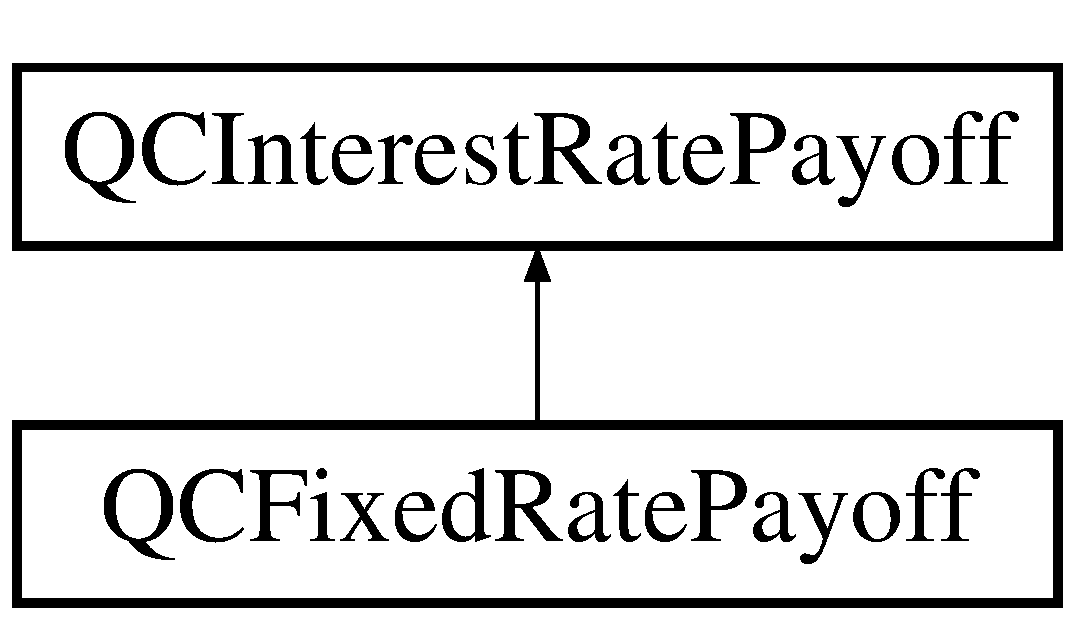
\includegraphics[height=2.000000cm]{class_q_c_fixed_rate_payoff}
\end{center}
\end{figure}
\subsection*{Public Member Functions}
\begin{DoxyCompactItemize}
\item 
\hypertarget{class_q_c_fixed_rate_payoff_a2347ff4dfef65aeda3a9f890cd83a3d8}{{\bfseries Q\+C\+Fixed\+Rate\+Payoff} (\hyperlink{_q_c_definitions_8h_ae6a21ad26d19e482e3b01179cbc05298}{Q\+C\+Intrst\+Rt\+Shrd\+Ptr} fixed\+Rate, shared\+\_\+ptr$<$ \hyperlink{class_q_c_interest_rate_leg}{Q\+C\+Interest\+Rate\+Leg} $>$ ir\+Leg, \hyperlink{_q_c_definitions_8h_a4b4fb466e49550e3dfd40003562cd19d}{Q\+C\+Int\+Rt\+Crv\+Shrd\+Ptr} discount\+Curve, \hyperlink{class_q_c_date}{Q\+C\+Date} value\+Date, \hyperlink{_q_c_definitions_8h_a6a601ffd693c05dd81309e3dca08b8f5}{Q\+C\+Time\+Series\+Shrd\+Ptr} fixing\+Data)}\label{class_q_c_fixed_rate_payoff_a2347ff4dfef65aeda3a9f890cd83a3d8}

\end{DoxyCompactItemize}
\subsection*{Protected Member Functions}
\begin{DoxyCompactItemize}
\item 
\hypertarget{class_q_c_fixed_rate_payoff_a7e20ddb8fb717480958a2eced9a4cf93}{virtual void {\bfseries \+\_\+set\+All\+Rates} () override}\label{class_q_c_fixed_rate_payoff_a7e20ddb8fb717480958a2eced9a4cf93}

\end{DoxyCompactItemize}
\subsection*{Additional Inherited Members}


\subsection{Detailed Description}


Definition at line 7 of file Q\+C\+Fixed\+Rate\+Payoff.\+h.



The documentation for this class was generated from the following file\+:\begin{DoxyCompactItemize}
\item 
include/Q\+C\+Fixed\+Rate\+Payoff.\+h\end{DoxyCompactItemize}

\hypertarget{class_q_c_floating_rate_payoff}{\section{Q\+C\+Floating\+Rate\+Payoff Class Reference}
\label{class_q_c_floating_rate_payoff}\index{Q\+C\+Floating\+Rate\+Payoff@{Q\+C\+Floating\+Rate\+Payoff}}
}
Inheritance diagram for Q\+C\+Floating\+Rate\+Payoff\+:\begin{figure}[H]
\begin{center}
\leavevmode
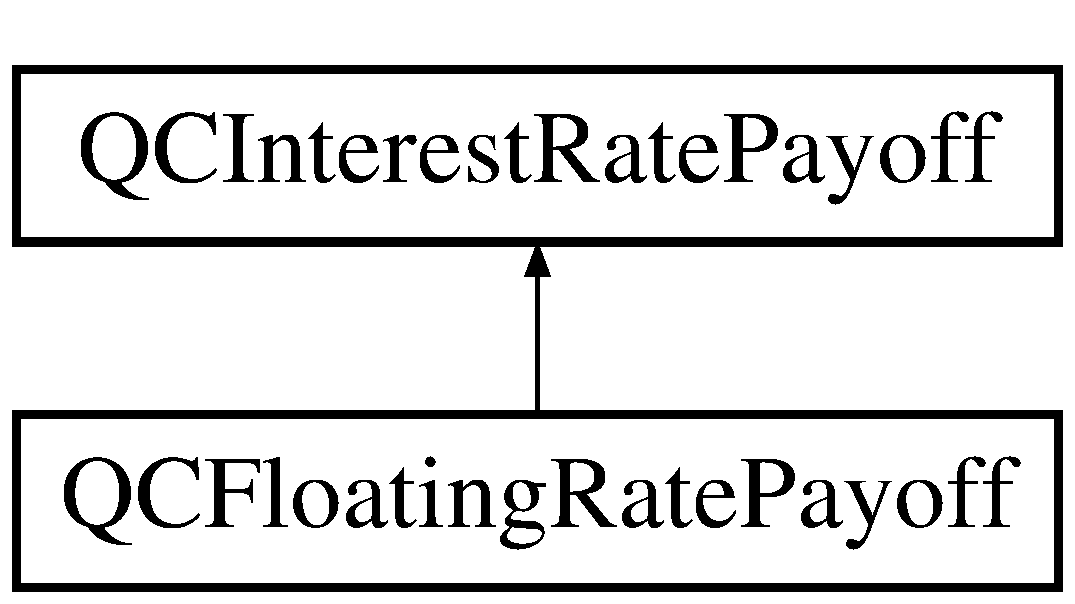
\includegraphics[height=2.000000cm]{class_q_c_floating_rate_payoff}
\end{center}
\end{figure}
\subsection*{Public Member Functions}
\begin{DoxyCompactItemize}
\item 
\hypertarget{class_q_c_floating_rate_payoff_ae06ea612302b5cb0cc88ec8a893e1fc1}{{\bfseries Q\+C\+Floating\+Rate\+Payoff} (\hyperlink{_q_c_definitions_8h_ae6a21ad26d19e482e3b01179cbc05298}{Q\+C\+Intrst\+Rt\+Shrd\+Ptr} floating\+Rate, double additive\+Spread, double multip\+Spread, shared\+\_\+ptr$<$ \hyperlink{class_q_c_interest_rate_leg}{Q\+C\+Interest\+Rate\+Leg} $>$ ir\+Leg, \hyperlink{_q_c_definitions_8h_a4b4fb466e49550e3dfd40003562cd19d}{Q\+C\+Int\+Rt\+Crv\+Shrd\+Ptr} projecting\+Curve, \hyperlink{_q_c_definitions_8h_a4b4fb466e49550e3dfd40003562cd19d}{Q\+C\+Int\+Rt\+Crv\+Shrd\+Ptr} discount\+Curve, \hyperlink{class_q_c_date}{Q\+C\+Date} value\+Date, \hyperlink{_q_c_definitions_8h_a6a601ffd693c05dd81309e3dca08b8f5}{Q\+C\+Time\+Series\+Shrd\+Ptr} fixing\+Data)}\label{class_q_c_floating_rate_payoff_ae06ea612302b5cb0cc88ec8a893e1fc1}

\item 
\hypertarget{class_q_c_floating_rate_payoff_a97363c05d03138861929b638a3485e4b}{double {\bfseries get\+Forward\+Rate\+At} (int n)}\label{class_q_c_floating_rate_payoff_a97363c05d03138861929b638a3485e4b}

\end{DoxyCompactItemize}
\subsection*{Protected Member Functions}
\begin{DoxyCompactItemize}
\item 
\hypertarget{class_q_c_floating_rate_payoff_a2c3247fbd8c5cf5398dfb465c42d84ca}{virtual void {\bfseries \+\_\+set\+All\+Rates} () override}\label{class_q_c_floating_rate_payoff_a2c3247fbd8c5cf5398dfb465c42d84ca}

\end{DoxyCompactItemize}
\subsection*{Protected Attributes}
\begin{DoxyCompactItemize}
\item 
\hypertarget{class_q_c_floating_rate_payoff_aa9db777cb92a9ee15b04f36dbdcb7320}{\hyperlink{_q_c_definitions_8h_a4b4fb466e49550e3dfd40003562cd19d}{Q\+C\+Int\+Rt\+Crv\+Shrd\+Ptr} {\bfseries \+\_\+projecting\+Curve}}\label{class_q_c_floating_rate_payoff_aa9db777cb92a9ee15b04f36dbdcb7320}

\item 
\hypertarget{class_q_c_floating_rate_payoff_a0ce362b934004dc4e1e60a0900b304ca}{double {\bfseries \+\_\+additive\+Spread}}\label{class_q_c_floating_rate_payoff_a0ce362b934004dc4e1e60a0900b304ca}

\item 
\hypertarget{class_q_c_floating_rate_payoff_a39f140ca9f175dc8ad9f471f6c11de81}{double {\bfseries \+\_\+multip\+Spread}}\label{class_q_c_floating_rate_payoff_a39f140ca9f175dc8ad9f471f6c11de81}

\item 
\hypertarget{class_q_c_floating_rate_payoff_aa6208ed72da94cb4cfb241f9fe78bdaf}{vector$<$ double $>$ {\bfseries \+\_\+forward\+Rates}}\label{class_q_c_floating_rate_payoff_aa6208ed72da94cb4cfb241f9fe78bdaf}

\end{DoxyCompactItemize}


\subsection{Detailed Description}


Definition at line 9 of file Q\+C\+Floating\+Rate\+Payoff.\+h.



The documentation for this class was generated from the following file\+:\begin{DoxyCompactItemize}
\item 
include/Q\+C\+Floating\+Rate\+Payoff.\+h\end{DoxyCompactItemize}

\hypertarget{class_q_c_icp_clf_payoff}{\section{Q\+C\+Icp\+Clf\+Payoff Class Reference}
\label{class_q_c_icp_clf_payoff}\index{Q\+C\+Icp\+Clf\+Payoff@{Q\+C\+Icp\+Clf\+Payoff}}
}
Inheritance diagram for Q\+C\+Icp\+Clf\+Payoff\+:\begin{figure}[H]
\begin{center}
\leavevmode
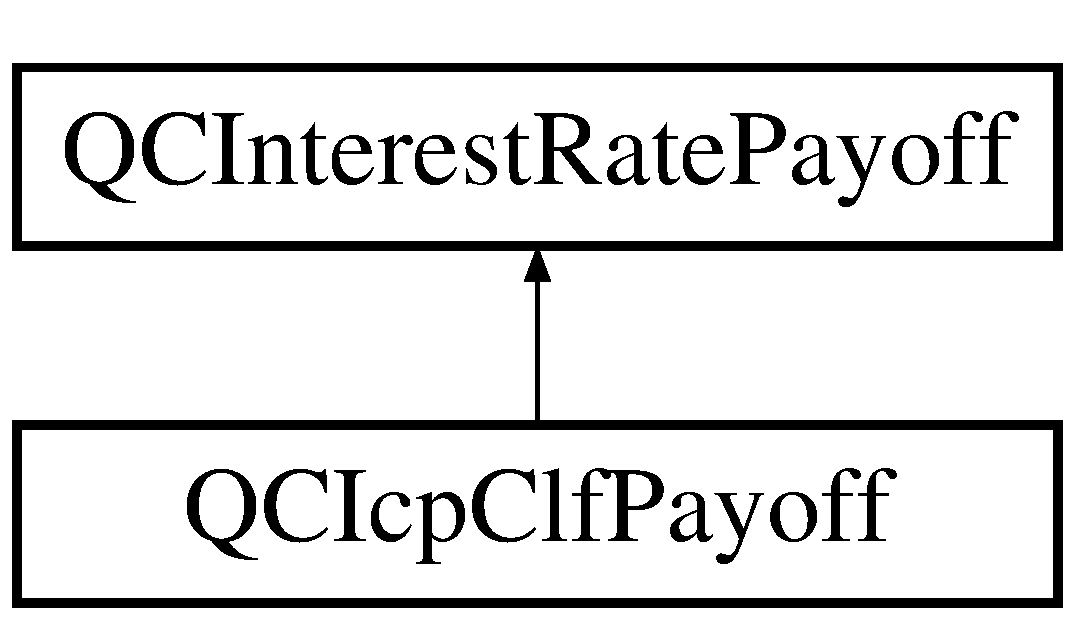
\includegraphics[height=2.000000cm]{class_q_c_icp_clf_payoff}
\end{center}
\end{figure}
\subsection*{Public Member Functions}
\begin{DoxyCompactItemize}
\item 
\hypertarget{class_q_c_icp_clf_payoff_a683899a85e390c596040712ac8692c46}{{\bfseries Q\+C\+Icp\+Clf\+Payoff} (\hyperlink{_q_c_definitions_8h_ae6a21ad26d19e482e3b01179cbc05298}{Q\+C\+Intrst\+Rt\+Shrd\+Ptr} floating\+Rate, double additive\+Spread, double multip\+Spread, shared\+\_\+ptr$<$ \hyperlink{class_q_c_interest_rate_leg}{Q\+C\+Interest\+Rate\+Leg} $>$ ir\+Leg, \hyperlink{_q_c_definitions_8h_a4b4fb466e49550e3dfd40003562cd19d}{Q\+C\+Int\+Rt\+Crv\+Shrd\+Ptr} projecting\+Curve, \hyperlink{_q_c_definitions_8h_a4b4fb466e49550e3dfd40003562cd19d}{Q\+C\+Int\+Rt\+Crv\+Shrd\+Ptr} discount\+Curve, \hyperlink{class_q_c_date}{Q\+C\+Date} value\+Date, \hyperlink{_q_c_definitions_8h_a6a601ffd693c05dd81309e3dca08b8f5}{Q\+C\+Time\+Series\+Shrd\+Ptr} fixing\+Data, \hyperlink{_q_c_definitions_8h_a6a601ffd693c05dd81309e3dca08b8f5}{Q\+C\+Time\+Series\+Shrd\+Ptr} fixing\+Data\+U\+F)}\label{class_q_c_icp_clf_payoff_a683899a85e390c596040712ac8692c46}

\item 
\hypertarget{class_q_c_icp_clf_payoff_a36aa6d8e71a0ef0357af1dd70b7b7d68}{double {\bfseries get\+Forward\+Rate\+At} (int n)}\label{class_q_c_icp_clf_payoff_a36aa6d8e71a0ef0357af1dd70b7b7d68}

\end{DoxyCompactItemize}
\subsection*{Protected Member Functions}
\begin{DoxyCompactItemize}
\item 
\hypertarget{class_q_c_icp_clf_payoff_af2a5eb4154c14eb2a1cb2d12e67d3744}{virtual void {\bfseries \+\_\+set\+All\+Rates} () override}\label{class_q_c_icp_clf_payoff_af2a5eb4154c14eb2a1cb2d12e67d3744}

\end{DoxyCompactItemize}
\subsection*{Protected Attributes}
\begin{DoxyCompactItemize}
\item 
\hypertarget{class_q_c_icp_clf_payoff_a038f8186cfc33b972362c8eb4843b3b8}{double {\bfseries \+\_\+additive\+Spread}}\label{class_q_c_icp_clf_payoff_a038f8186cfc33b972362c8eb4843b3b8}

\item 
\hypertarget{class_q_c_icp_clf_payoff_acd6dfaf17c08d75c978d1077ce713bc2}{double {\bfseries \+\_\+multip\+Spread}}\label{class_q_c_icp_clf_payoff_acd6dfaf17c08d75c978d1077ce713bc2}

\item 
\hypertarget{class_q_c_icp_clf_payoff_a4d724785270e7434537d2d7bfe5ef90f}{vector$<$ double $>$ {\bfseries \+\_\+forward\+Rates}}\label{class_q_c_icp_clf_payoff_a4d724785270e7434537d2d7bfe5ef90f}

\item 
\hypertarget{class_q_c_icp_clf_payoff_a866088bdf4d4aaba48b96e6f97b0a7a6}{\hyperlink{_q_c_definitions_8h_a6a601ffd693c05dd81309e3dca08b8f5}{Q\+C\+Time\+Series\+Shrd\+Ptr} {\bfseries \+\_\+fixing\+Data\+U\+F}}\label{class_q_c_icp_clf_payoff_a866088bdf4d4aaba48b96e6f97b0a7a6}

\end{DoxyCompactItemize}


\subsection{Detailed Description}


Definition at line 5 of file Q\+C\+Icp\+Clf\+Payoff.\+h.



The documentation for this class was generated from the following file\+:\begin{DoxyCompactItemize}
\item 
include/Q\+C\+Icp\+Clf\+Payoff.\+h\end{DoxyCompactItemize}

\hypertarget{class_q_c_icp_clp_payoff}{\section{Q\+C\+Icp\+Clp\+Payoff Class Reference}
\label{class_q_c_icp_clp_payoff}\index{Q\+C\+Icp\+Clp\+Payoff@{Q\+C\+Icp\+Clp\+Payoff}}
}
Inheritance diagram for Q\+C\+Icp\+Clp\+Payoff\+:\begin{figure}[H]
\begin{center}
\leavevmode
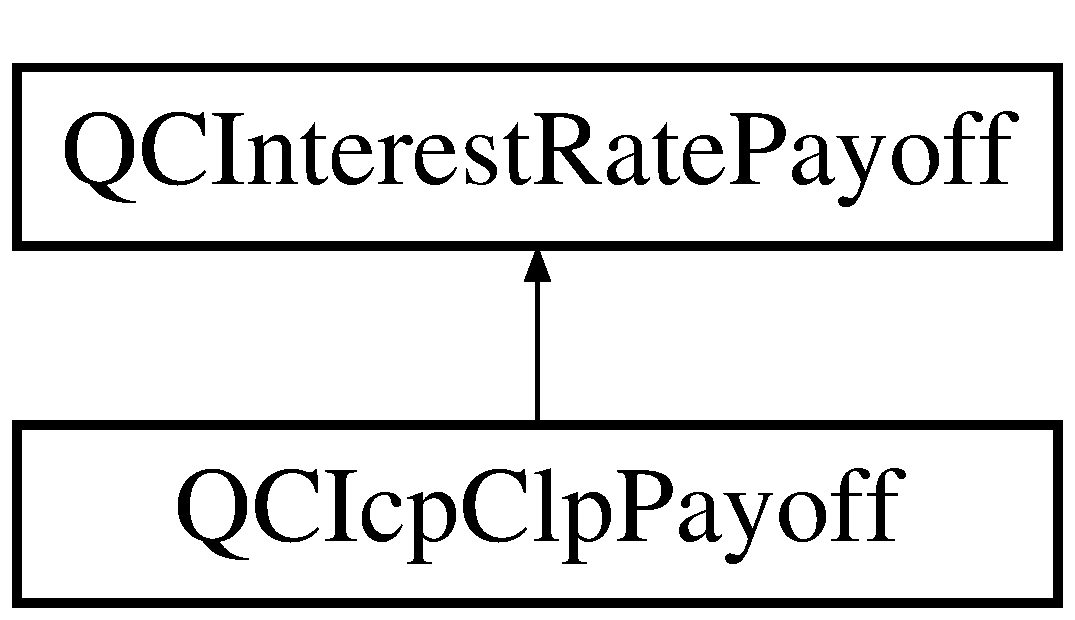
\includegraphics[height=2.000000cm]{class_q_c_icp_clp_payoff}
\end{center}
\end{figure}
\subsection*{Public Member Functions}
\begin{DoxyCompactItemize}
\item 
\hypertarget{class_q_c_icp_clp_payoff_a59a723c0acdd41ad77877210c73a5fd1}{{\bfseries Q\+C\+Icp\+Clp\+Payoff} (\hyperlink{_q_c_definitions_8h_ae6a21ad26d19e482e3b01179cbc05298}{Q\+C\+Intrst\+Rt\+Shrd\+Ptr} floating\+Rate, double additive\+Spread, double multip\+Spread, shared\+\_\+ptr$<$ \hyperlink{class_q_c_interest_rate_leg}{Q\+C\+Interest\+Rate\+Leg} $>$ ir\+Leg, \hyperlink{_q_c_definitions_8h_a4b4fb466e49550e3dfd40003562cd19d}{Q\+C\+Int\+Rt\+Crv\+Shrd\+Ptr} projecting\+Curve, \hyperlink{_q_c_definitions_8h_a4b4fb466e49550e3dfd40003562cd19d}{Q\+C\+Int\+Rt\+Crv\+Shrd\+Ptr} discount\+Curve, \hyperlink{class_q_c_date}{Q\+C\+Date} value\+Date, \hyperlink{_q_c_definitions_8h_a6a601ffd693c05dd81309e3dca08b8f5}{Q\+C\+Time\+Series\+Shrd\+Ptr} fixing\+Data)}\label{class_q_c_icp_clp_payoff_a59a723c0acdd41ad77877210c73a5fd1}

\item 
\hypertarget{class_q_c_icp_clp_payoff_a263487dea487c5f3e326797dda3ad90b}{double {\bfseries get\+Forward\+Rate\+At} (int n)}\label{class_q_c_icp_clp_payoff_a263487dea487c5f3e326797dda3ad90b}

\end{DoxyCompactItemize}
\subsection*{Protected Member Functions}
\begin{DoxyCompactItemize}
\item 
\hypertarget{class_q_c_icp_clp_payoff_af962eed7dbb1968c86575fb7d795f066}{virtual void {\bfseries \+\_\+set\+All\+Rates} () override}\label{class_q_c_icp_clp_payoff_af962eed7dbb1968c86575fb7d795f066}

\end{DoxyCompactItemize}
\subsection*{Protected Attributes}
\begin{DoxyCompactItemize}
\item 
\hypertarget{class_q_c_icp_clp_payoff_a5382209d1d84da225e9e5e32a2b79ca0}{double {\bfseries \+\_\+additive\+Spread}}\label{class_q_c_icp_clp_payoff_a5382209d1d84da225e9e5e32a2b79ca0}

\item 
\hypertarget{class_q_c_icp_clp_payoff_a3291226b6bff6459f8754f15229b4abf}{double {\bfseries \+\_\+multip\+Spread}}\label{class_q_c_icp_clp_payoff_a3291226b6bff6459f8754f15229b4abf}

\item 
\hypertarget{class_q_c_icp_clp_payoff_a37e674eebfd2650bcf4fead468724125}{vector$<$ double $>$ {\bfseries \+\_\+forward\+Rates}}\label{class_q_c_icp_clp_payoff_a37e674eebfd2650bcf4fead468724125}

\end{DoxyCompactItemize}


\subsection{Detailed Description}


Definition at line 5 of file Q\+C\+Icp\+Clp\+Payoff.\+h.



The documentation for this class was generated from the following file\+:\begin{DoxyCompactItemize}
\item 
include/Q\+C\+Icp\+Clp\+Payoff.\+h\end{DoxyCompactItemize}

\hypertarget{class_q_c_interest_rate}{\section{Q\+C\+Interest\+Rate Class Reference}
\label{class_q_c_interest_rate}\index{Q\+C\+Interest\+Rate@{Q\+C\+Interest\+Rate}}
}
\subsection*{Public Member Functions}
\begin{DoxyCompactItemize}
\item 
\hypertarget{class_q_c_interest_rate_a10814e414dfe84d64158801cdd0f6e8a}{{\bfseries Q\+C\+Interest\+Rate} (double value, \hyperlink{_q_c_definitions_8h_abcfd4021c75f633fa6d7a4552ced4a38}{Q\+C\+Yr\+Frctn\+Shrd\+Ptr} year\+Fraction, \hyperlink{_q_c_definitions_8h_a2085df477a1aafaad6ed79890607f447}{Q\+C\+Wlth\+Fctr\+Shrd\+Ptr} wealth\+Factor)}\label{class_q_c_interest_rate_a10814e414dfe84d64158801cdd0f6e8a}

\item 
\hypertarget{class_q_c_interest_rate_ae87a6e803d5b0ba27a223dcc1c52ada4}{double {\bfseries get\+Value} ()}\label{class_q_c_interest_rate_ae87a6e803d5b0ba27a223dcc1c52ada4}

\item 
\hypertarget{class_q_c_interest_rate_ab718b93038f3be85b7c0d4cab9d92d8d}{void {\bfseries set\+Value} (double value)}\label{class_q_c_interest_rate_ab718b93038f3be85b7c0d4cab9d92d8d}

\item 
\hypertarget{class_q_c_interest_rate_a1245a1aa2d41304ad9134e06ed7663d3}{double {\bfseries wf} (\hyperlink{class_q_c_date}{Q\+C\+Date} \&start\+Date, \hyperlink{class_q_c_date}{Q\+C\+Date} \&end\+Date)}\label{class_q_c_interest_rate_a1245a1aa2d41304ad9134e06ed7663d3}

\item 
\hypertarget{class_q_c_interest_rate_a0607f8abed935ee8f036f81e3be96223}{double {\bfseries wf} (long days)}\label{class_q_c_interest_rate_a0607f8abed935ee8f036f81e3be96223}

\item 
\hypertarget{class_q_c_interest_rate_ae58c028cc811c1a6a560ed9985a98210}{double {\bfseries dwf} (\hyperlink{class_q_c_date}{Q\+C\+Date} \&start\+Date, \hyperlink{class_q_c_date}{Q\+C\+Date} \&end\+Date)}\label{class_q_c_interest_rate_ae58c028cc811c1a6a560ed9985a98210}

\item 
\hypertarget{class_q_c_interest_rate_a99365541cdc1fdea589f7ded97d861c8}{double {\bfseries dwf} (long days)}\label{class_q_c_interest_rate_a99365541cdc1fdea589f7ded97d861c8}

\item 
\hypertarget{class_q_c_interest_rate_aee3f65ca6b55dab624646985171f9032}{double {\bfseries get\+Rate\+From\+Wf} (double wf, \hyperlink{class_q_c_date}{Q\+C\+Date} \&start\+Date, \hyperlink{class_q_c_date}{Q\+C\+Date} \&end\+Date)}\label{class_q_c_interest_rate_aee3f65ca6b55dab624646985171f9032}

\item 
\hypertarget{class_q_c_interest_rate_ac694edd3bd07d3538ef8a37fd19cd3ba}{double {\bfseries get\+Rate\+From\+Wf} (double wf, long days)}\label{class_q_c_interest_rate_ac694edd3bd07d3538ef8a37fd19cd3ba}

\item 
\hypertarget{class_q_c_interest_rate_a8370686c8615f04bfa39560bba1488a1}{double {\bfseries yf} (\hyperlink{class_q_c_date}{Q\+C\+Date} \&start\+Date, \hyperlink{class_q_c_date}{Q\+C\+Date} \&end\+Date)}\label{class_q_c_interest_rate_a8370686c8615f04bfa39560bba1488a1}

\end{DoxyCompactItemize}


\subsection{Detailed Description}


Definition at line 8 of file Q\+C\+Interest\+Rate.\+h.



The documentation for this class was generated from the following file\+:\begin{DoxyCompactItemize}
\item 
include/Q\+C\+Interest\+Rate.\+h\end{DoxyCompactItemize}

\hypertarget{class_q_c_interest_rate_curve}{\section{Q\+C\+Interest\+Rate\+Curve Class Reference}
\label{class_q_c_interest_rate_curve}\index{Q\+C\+Interest\+Rate\+Curve@{Q\+C\+Interest\+Rate\+Curve}}
}


Clase base abstracta para todas las curvas de tasas de interés.  




{\ttfamily \#include $<$Q\+C\+Interest\+Rate\+Curve.\+h$>$}

Inheritance diagram for Q\+C\+Interest\+Rate\+Curve\+:\begin{figure}[H]
\begin{center}
\leavevmode
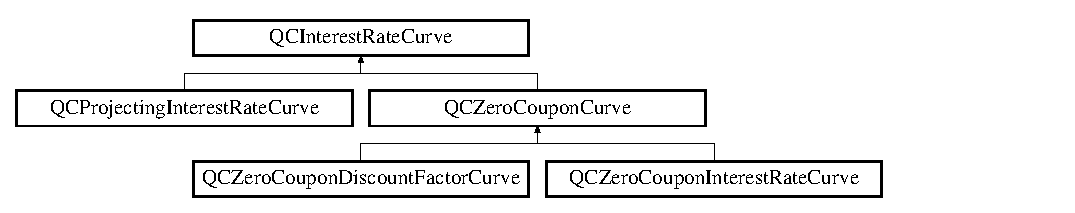
\includegraphics[height=2.413793cm]{class_q_c_interest_rate_curve}
\end{center}
\end{figure}
\subsection*{Public Types}
\begin{DoxyCompactItemize}
\item 
enum \hyperlink{class_q_c_interest_rate_curve_a68e2145ab0bc68344bcfcdfaf592fb63}{Q\+C\+Type\+Interest\+Rate\+Curve} \{ \hyperlink{class_q_c_interest_rate_curve_a68e2145ab0bc68344bcfcdfaf592fb63a877e81812e983cf935de5f225d025305}{qc\+Projecting\+Curve}, 
\hyperlink{class_q_c_interest_rate_curve_a68e2145ab0bc68344bcfcdfaf592fb63a22386a704b2c20f8fe7e4b4461cbc22d}{qc\+Zero\+Coupon\+Curve}, 
\hyperlink{class_q_c_interest_rate_curve_a68e2145ab0bc68344bcfcdfaf592fb63a37f65bba40528ce332c6c24825e8ba17}{qc\+Discount\+Factor\+Curve}
 \}
\end{DoxyCompactItemize}
\subsection*{Public Member Functions}
\begin{DoxyCompactItemize}
\item 
\hyperlink{class_q_c_interest_rate_curve_a9fbbecad2b5f69e7b873569e118fbbec}{Q\+C\+Interest\+Rate\+Curve} (shared\+\_\+ptr$<$ \hyperlink{class_q_c_interpolator}{Q\+C\+Interpolator} $>$ curve, \hyperlink{class_q_c_interest_rate}{Q\+C\+Interest\+Rate} int\+Rate)
\item 
virtual double \hyperlink{class_q_c_interest_rate_curve_a0a73e8506d0706becd93b04c4499a9c6}{get\+Rate\+At} (long d)=0
\item 
virtual double \hyperlink{class_q_c_interest_rate_curve_abe670a951f0fca2273726d13ce9cda06}{get\+Discount\+Factor\+At} (long d)=0
\item 
virtual double \hyperlink{class_q_c_interest_rate_curve_a66e79c4ed2e08916f14bbbfb5d1d3c96}{get\+Forward\+Rate} (\hyperlink{class_q_c_interest_rate}{Q\+C\+Interest\+Rate} \&int\+Rate, long d1, long d2)=0
\item 
virtual double \hyperlink{class_q_c_interest_rate_curve_af4c22b08db379ea8ce825f9999e2bc34}{get\+Forward\+Rate} (long d1, long d2)=0
\item 
virtual double \hyperlink{class_q_c_interest_rate_curve_a36c88024727170486082197f1abff78e}{get\+Forward\+Wf} (long d1, long d2)=0
\item 
virtual double \hyperlink{class_q_c_interest_rate_curve_a07a3e60dc1e7d25a025fc587b055c813}{df\+Derivative\+At} (unsigned int index)=0
\item 
virtual double \hyperlink{class_q_c_interest_rate_curve_a8aa3dcfb5a3ce169094db4e2f0849a94}{fwd\+Wf\+Derivative\+At} (unsigned int index)=0
\item 
long \hyperlink{class_q_c_interest_rate_curve_ad3c05d050bf861646fe49c1ac964a771}{get\+Length} ()
\item 
virtual \hyperlink{class_q_c_interest_rate_curve_a96a9bdf5a149ffe8acdabf3d136778e1}{$\sim$\+Q\+C\+Interest\+Rate\+Curve} ()
\end{DoxyCompactItemize}
\subsection*{Protected Attributes}
\begin{DoxyCompactItemize}
\item 
shared\+\_\+ptr$<$ \hyperlink{class_q_c_interpolator}{Q\+C\+Interpolator} $>$ \hyperlink{class_q_c_interest_rate_curve_af788dba3aafd45c2275e7f049df8f7ee}{\+\_\+curve}
\item 
\hypertarget{class_q_c_interest_rate_curve_a50f92300e3a22e662bdecd3c51ece386}{\hyperlink{class_q_c_interest_rate}{Q\+C\+Interest\+Rate} {\bfseries \+\_\+int\+Rate}}\label{class_q_c_interest_rate_curve_a50f92300e3a22e662bdecd3c51ece386}

\item 
vector$<$ double $>$ \hyperlink{class_q_c_interest_rate_curve_a654de5d23f8bb2b76df9edb70acf9fca}{\+\_\+df\+Derivatives}
\item 
vector$<$ double $>$ \hyperlink{class_q_c_interest_rate_curve_ae343e0126c675330a0fa15611db8428b}{\+\_\+fwd\+Wf\+Derivatives}
\end{DoxyCompactItemize}


\subsection{Detailed Description}
Clase base abstracta para todas las curvas de tasas de interés. 

\begin{DoxyAuthor}{Author}
Alvaro Díaz
\end{DoxyAuthor}
Esta clase define varios métodos que las clases derivadas deben implementar. Los distintos tipos de curvas (descuento, proyección, por factores o tasas) se derivan de ésta. 

Definition at line 15 of file Q\+C\+Interest\+Rate\+Curve.\+h.



\subsection{Member Enumeration Documentation}
\hypertarget{class_q_c_interest_rate_curve_a68e2145ab0bc68344bcfcdfaf592fb63}{\index{Q\+C\+Interest\+Rate\+Curve@{Q\+C\+Interest\+Rate\+Curve}!Q\+C\+Type\+Interest\+Rate\+Curve@{Q\+C\+Type\+Interest\+Rate\+Curve}}
\index{Q\+C\+Type\+Interest\+Rate\+Curve@{Q\+C\+Type\+Interest\+Rate\+Curve}!Q\+C\+Interest\+Rate\+Curve@{Q\+C\+Interest\+Rate\+Curve}}
\subsubsection[{Q\+C\+Type\+Interest\+Rate\+Curve}]{\setlength{\rightskip}{0pt plus 5cm}enum {\bf Q\+C\+Interest\+Rate\+Curve\+::\+Q\+C\+Type\+Interest\+Rate\+Curve}}}\label{class_q_c_interest_rate_curve_a68e2145ab0bc68344bcfcdfaf592fb63}
Enumera los distintos tipos de curvas de tasas de interés. \begin{Desc}
\item[Enumerator]\par
\begin{description}
\index{qc\+Projecting\+Curve@{qc\+Projecting\+Curve}!Q\+C\+Interest\+Rate\+Curve@{Q\+C\+Interest\+Rate\+Curve}}\index{Q\+C\+Interest\+Rate\+Curve@{Q\+C\+Interest\+Rate\+Curve}!qc\+Projecting\+Curve@{qc\+Projecting\+Curve}}\item[{\em 
\hypertarget{class_q_c_interest_rate_curve_a68e2145ab0bc68344bcfcdfaf592fb63a877e81812e983cf935de5f225d025305}{qc\+Projecting\+Curve}\label{class_q_c_interest_rate_curve_a68e2145ab0bc68344bcfcdfaf592fb63a877e81812e983cf935de5f225d025305}
}]Curva de proyección. Al interpolar se obtiene una tasa forward de un tenor predefinido. \index{qc\+Zero\+Coupon\+Curve@{qc\+Zero\+Coupon\+Curve}!Q\+C\+Interest\+Rate\+Curve@{Q\+C\+Interest\+Rate\+Curve}}\index{Q\+C\+Interest\+Rate\+Curve@{Q\+C\+Interest\+Rate\+Curve}!qc\+Zero\+Coupon\+Curve@{qc\+Zero\+Coupon\+Curve}}\item[{\em 
\hypertarget{class_q_c_interest_rate_curve_a68e2145ab0bc68344bcfcdfaf592fb63a22386a704b2c20f8fe7e4b4461cbc22d}{qc\+Zero\+Coupon\+Curve}\label{class_q_c_interest_rate_curve_a68e2145ab0bc68344bcfcdfaf592fb63a22386a704b2c20f8fe7e4b4461cbc22d}
}]Curva cero cupón. Se especifica entregando los plazos en días y valores de las tasas. \index{qc\+Discount\+Factor\+Curve@{qc\+Discount\+Factor\+Curve}!Q\+C\+Interest\+Rate\+Curve@{Q\+C\+Interest\+Rate\+Curve}}\index{Q\+C\+Interest\+Rate\+Curve@{Q\+C\+Interest\+Rate\+Curve}!qc\+Discount\+Factor\+Curve@{qc\+Discount\+Factor\+Curve}}\item[{\em 
\hypertarget{class_q_c_interest_rate_curve_a68e2145ab0bc68344bcfcdfaf592fb63a37f65bba40528ce332c6c24825e8ba17}{qc\+Discount\+Factor\+Curve}\label{class_q_c_interest_rate_curve_a68e2145ab0bc68344bcfcdfaf592fb63a37f65bba40528ce332c6c24825e8ba17}
}]Curva de factores de descuento. Se especifica entregando los plazos en días y los valores de los factores de descuento. \end{description}
\end{Desc}


Definition at line 21 of file Q\+C\+Interest\+Rate\+Curve.\+h.



\subsection{Constructor \& Destructor Documentation}
\hypertarget{class_q_c_interest_rate_curve_a9fbbecad2b5f69e7b873569e118fbbec}{\index{Q\+C\+Interest\+Rate\+Curve@{Q\+C\+Interest\+Rate\+Curve}!Q\+C\+Interest\+Rate\+Curve@{Q\+C\+Interest\+Rate\+Curve}}
\index{Q\+C\+Interest\+Rate\+Curve@{Q\+C\+Interest\+Rate\+Curve}!Q\+C\+Interest\+Rate\+Curve@{Q\+C\+Interest\+Rate\+Curve}}
\subsubsection[{Q\+C\+Interest\+Rate\+Curve}]{\setlength{\rightskip}{0pt plus 5cm}Q\+C\+Interest\+Rate\+Curve\+::\+Q\+C\+Interest\+Rate\+Curve (
\begin{DoxyParamCaption}
\item[{shared\+\_\+ptr$<$ {\bf Q\+C\+Interpolator} $>$}]{curve, }
\item[{{\bf Q\+C\+Interest\+Rate}}]{int\+Rate}
\end{DoxyParamCaption}
)\hspace{0.3cm}{\ttfamily [inline]}}}\label{class_q_c_interest_rate_curve_a9fbbecad2b5f69e7b873569e118fbbec}
Constructor de la clase. 
\begin{DoxyParams}{Parameters}
{\em curve} & plazos y valores (tasas o factores de descuento) de la curva junto con el método de interpolación seleccionado. \\
\hline
{\em int\+Rate} & contiene el tipo de las tasas de interés de la curva. \\
\hline
\end{DoxyParams}


Definition at line 40 of file Q\+C\+Interest\+Rate\+Curve.\+h.

\hypertarget{class_q_c_interest_rate_curve_a96a9bdf5a149ffe8acdabf3d136778e1}{\index{Q\+C\+Interest\+Rate\+Curve@{Q\+C\+Interest\+Rate\+Curve}!````~Q\+C\+Interest\+Rate\+Curve@{$\sim$\+Q\+C\+Interest\+Rate\+Curve}}
\index{````~Q\+C\+Interest\+Rate\+Curve@{$\sim$\+Q\+C\+Interest\+Rate\+Curve}!Q\+C\+Interest\+Rate\+Curve@{Q\+C\+Interest\+Rate\+Curve}}
\subsubsection[{$\sim$\+Q\+C\+Interest\+Rate\+Curve}]{\setlength{\rightskip}{0pt plus 5cm}virtual Q\+C\+Interest\+Rate\+Curve\+::$\sim$\+Q\+C\+Interest\+Rate\+Curve (
\begin{DoxyParamCaption}
{}
\end{DoxyParamCaption}
)\hspace{0.3cm}{\ttfamily [inline]}, {\ttfamily [virtual]}}}\label{class_q_c_interest_rate_curve_a96a9bdf5a149ffe8acdabf3d136778e1}
Destructor de la clase. 

Definition at line 110 of file Q\+C\+Interest\+Rate\+Curve.\+h.



\subsection{Member Function Documentation}
\hypertarget{class_q_c_interest_rate_curve_a07a3e60dc1e7d25a025fc587b055c813}{\index{Q\+C\+Interest\+Rate\+Curve@{Q\+C\+Interest\+Rate\+Curve}!df\+Derivative\+At@{df\+Derivative\+At}}
\index{df\+Derivative\+At@{df\+Derivative\+At}!Q\+C\+Interest\+Rate\+Curve@{Q\+C\+Interest\+Rate\+Curve}}
\subsubsection[{df\+Derivative\+At}]{\setlength{\rightskip}{0pt plus 5cm}virtual double Q\+C\+Interest\+Rate\+Curve\+::df\+Derivative\+At (
\begin{DoxyParamCaption}
\item[{unsigned int}]{index}
\end{DoxyParamCaption}
)\hspace{0.3cm}{\ttfamily [pure virtual]}}}\label{class_q_c_interest_rate_curve_a07a3e60dc1e7d25a025fc587b055c813}
Este método es un getter que retorna la derivada del último factor de capitalización calculado. \begin{DoxyReturn}{Returns}
valor de la derivada. 
\end{DoxyReturn}


Implemented in \hyperlink{class_q_c_zero_coupon_curve_afe641c34018bcc867b498f67e7c7d19d}{Q\+C\+Zero\+Coupon\+Curve}, \hyperlink{class_q_c_projecting_interest_rate_curve_aa32b5f4d4bea4565e3610bda00ed8d06}{Q\+C\+Projecting\+Interest\+Rate\+Curve}, and \hyperlink{class_q_c_zero_coupon_interest_rate_curve_a24ae7f1a9021c24984c5c002d0df1494}{Q\+C\+Zero\+Coupon\+Interest\+Rate\+Curve}.

\hypertarget{class_q_c_interest_rate_curve_a8aa3dcfb5a3ce169094db4e2f0849a94}{\index{Q\+C\+Interest\+Rate\+Curve@{Q\+C\+Interest\+Rate\+Curve}!fwd\+Wf\+Derivative\+At@{fwd\+Wf\+Derivative\+At}}
\index{fwd\+Wf\+Derivative\+At@{fwd\+Wf\+Derivative\+At}!Q\+C\+Interest\+Rate\+Curve@{Q\+C\+Interest\+Rate\+Curve}}
\subsubsection[{fwd\+Wf\+Derivative\+At}]{\setlength{\rightskip}{0pt plus 5cm}virtual double Q\+C\+Interest\+Rate\+Curve\+::fwd\+Wf\+Derivative\+At (
\begin{DoxyParamCaption}
\item[{unsigned int}]{index}
\end{DoxyParamCaption}
)\hspace{0.3cm}{\ttfamily [pure virtual]}}}\label{class_q_c_interest_rate_curve_a8aa3dcfb5a3ce169094db4e2f0849a94}
Este método es un getter que retorna la derivada del último factor de capitalización forward calculado. \begin{DoxyReturn}{Returns}
valor de la derivada. 
\end{DoxyReturn}


Implemented in \hyperlink{class_q_c_projecting_interest_rate_curve_ad6b67e23665886cdcf91957fe12e10d8}{Q\+C\+Projecting\+Interest\+Rate\+Curve}, \hyperlink{class_q_c_zero_coupon_interest_rate_curve_a043fd0690f9a941b5268e1b1f7d07ef1}{Q\+C\+Zero\+Coupon\+Interest\+Rate\+Curve}, and \hyperlink{class_q_c_zero_coupon_discount_factor_curve_a336906041380286ee1f8257d9a97e486}{Q\+C\+Zero\+Coupon\+Discount\+Factor\+Curve}.

\hypertarget{class_q_c_interest_rate_curve_abe670a951f0fca2273726d13ce9cda06}{\index{Q\+C\+Interest\+Rate\+Curve@{Q\+C\+Interest\+Rate\+Curve}!get\+Discount\+Factor\+At@{get\+Discount\+Factor\+At}}
\index{get\+Discount\+Factor\+At@{get\+Discount\+Factor\+At}!Q\+C\+Interest\+Rate\+Curve@{Q\+C\+Interest\+Rate\+Curve}}
\subsubsection[{get\+Discount\+Factor\+At}]{\setlength{\rightskip}{0pt plus 5cm}virtual double Q\+C\+Interest\+Rate\+Curve\+::get\+Discount\+Factor\+At (
\begin{DoxyParamCaption}
\item[{long}]{d}
\end{DoxyParamCaption}
)\hspace{0.3cm}{\ttfamily [pure virtual]}}}\label{class_q_c_interest_rate_curve_abe670a951f0fca2273726d13ce9cda06}
Retorna el factor de descuento interpolado al plazo d. 
\begin{DoxyParams}{Parameters}
{\em d} & plazo a interpolar \\
\hline
\end{DoxyParams}
\begin{DoxyReturn}{Returns}
valor del factor de descuento interpolado. 
\end{DoxyReturn}


Implemented in \hyperlink{class_q_c_zero_coupon_curve_ac7546a18d2fe462e14ddae2d8c87b7c5}{Q\+C\+Zero\+Coupon\+Curve}, \hyperlink{class_q_c_projecting_interest_rate_curve_a777da5100b3dd412e9764c6129c6715b}{Q\+C\+Projecting\+Interest\+Rate\+Curve}, \hyperlink{class_q_c_zero_coupon_discount_factor_curve_a1c09de3cfa88c80f8ece2feac6905c0d}{Q\+C\+Zero\+Coupon\+Discount\+Factor\+Curve}, and \hyperlink{class_q_c_zero_coupon_interest_rate_curve_af3a5bec430ce4a652831b47ccbcca354}{Q\+C\+Zero\+Coupon\+Interest\+Rate\+Curve}.

\hypertarget{class_q_c_interest_rate_curve_a66e79c4ed2e08916f14bbbfb5d1d3c96}{\index{Q\+C\+Interest\+Rate\+Curve@{Q\+C\+Interest\+Rate\+Curve}!get\+Forward\+Rate@{get\+Forward\+Rate}}
\index{get\+Forward\+Rate@{get\+Forward\+Rate}!Q\+C\+Interest\+Rate\+Curve@{Q\+C\+Interest\+Rate\+Curve}}
\subsubsection[{get\+Forward\+Rate}]{\setlength{\rightskip}{0pt plus 5cm}virtual double Q\+C\+Interest\+Rate\+Curve\+::get\+Forward\+Rate (
\begin{DoxyParamCaption}
\item[{{\bf Q\+C\+Interest\+Rate} \&}]{int\+Rate, }
\item[{long}]{d1, }
\item[{long}]{d2}
\end{DoxyParamCaption}
)\hspace{0.3cm}{\ttfamily [pure virtual]}}}\label{class_q_c_interest_rate_curve_a66e79c4ed2e08916f14bbbfb5d1d3c96}
Retorna la tasa forward entre los plazos d1 y d2 en la convención de int\+Rate. 
\begin{DoxyParams}{Parameters}
{\em int\+Rate} & convención de la tasa forward que se debe calcular. \\
\hline
{\em d1} & plazo más corto de la tasa forward. \\
\hline
{\em d2} & plazo más largo de la tasa forward. \\
\hline
\end{DoxyParams}
\begin{DoxyReturn}{Returns}
valor de la tasa forward calculada. Probablemente este método puede mejorarse haciendo que retorne void y el valor de la tasa forward calculada se almacene dentro de la variable int\+Rate. 
\end{DoxyReturn}


Implemented in \hyperlink{class_q_c_projecting_interest_rate_curve_a2f01098cb4e3c2ba6163fb9bef4a6b66}{Q\+C\+Projecting\+Interest\+Rate\+Curve}, \hyperlink{class_q_c_zero_coupon_discount_factor_curve_a444623664ba1bd0d0855bc11cbde64dd}{Q\+C\+Zero\+Coupon\+Discount\+Factor\+Curve}, and \hyperlink{class_q_c_zero_coupon_interest_rate_curve_a623b9416cc04c5a2a59b1279f20d3220}{Q\+C\+Zero\+Coupon\+Interest\+Rate\+Curve}.

\hypertarget{class_q_c_interest_rate_curve_af4c22b08db379ea8ce825f9999e2bc34}{\index{Q\+C\+Interest\+Rate\+Curve@{Q\+C\+Interest\+Rate\+Curve}!get\+Forward\+Rate@{get\+Forward\+Rate}}
\index{get\+Forward\+Rate@{get\+Forward\+Rate}!Q\+C\+Interest\+Rate\+Curve@{Q\+C\+Interest\+Rate\+Curve}}
\subsubsection[{get\+Forward\+Rate}]{\setlength{\rightskip}{0pt plus 5cm}virtual double Q\+C\+Interest\+Rate\+Curve\+::get\+Forward\+Rate (
\begin{DoxyParamCaption}
\item[{long}]{d1, }
\item[{long}]{d2}
\end{DoxyParamCaption}
)\hspace{0.3cm}{\ttfamily [pure virtual]}}}\label{class_q_c_interest_rate_curve_af4c22b08db379ea8ce825f9999e2bc34}
Retorna la tasa forward entre los plazos d1 y d2 en la convención de las tasas de la curva. 
\begin{DoxyParams}{Parameters}
{\em d1} & plazo más corto de la tasa forward. \\
\hline
{\em d2} & plazo más largo de la tasa forward. \\
\hline
\end{DoxyParams}
\begin{DoxyReturn}{Returns}
valor de la tasa forward calculada. 
\end{DoxyReturn}


Implemented in \hyperlink{class_q_c_projecting_interest_rate_curve_a07a0b96ca283abb7f3e0a79432bcdee9}{Q\+C\+Projecting\+Interest\+Rate\+Curve}, \hyperlink{class_q_c_zero_coupon_discount_factor_curve_a9287f90424bfa40964835df46d3e3601}{Q\+C\+Zero\+Coupon\+Discount\+Factor\+Curve}, and \hyperlink{class_q_c_zero_coupon_interest_rate_curve_a17770bb86b17de6336be98b622ff992b}{Q\+C\+Zero\+Coupon\+Interest\+Rate\+Curve}.

\hypertarget{class_q_c_interest_rate_curve_a36c88024727170486082197f1abff78e}{\index{Q\+C\+Interest\+Rate\+Curve@{Q\+C\+Interest\+Rate\+Curve}!get\+Forward\+Wf@{get\+Forward\+Wf}}
\index{get\+Forward\+Wf@{get\+Forward\+Wf}!Q\+C\+Interest\+Rate\+Curve@{Q\+C\+Interest\+Rate\+Curve}}
\subsubsection[{get\+Forward\+Wf}]{\setlength{\rightskip}{0pt plus 5cm}virtual double Q\+C\+Interest\+Rate\+Curve\+::get\+Forward\+Wf (
\begin{DoxyParamCaption}
\item[{long}]{d1, }
\item[{long}]{d2}
\end{DoxyParamCaption}
)\hspace{0.3cm}{\ttfamily [pure virtual]}}}\label{class_q_c_interest_rate_curve_a36c88024727170486082197f1abff78e}
Retorna la factor de capitalización forward entre los plazos d1 y d2. 
\begin{DoxyParams}{Parameters}
{\em d1} & plazo más corto del factor forward. \\
\hline
{\em d2} & plazo más largo del fcator forward. \\
\hline
\end{DoxyParams}
\begin{DoxyReturn}{Returns}
valor del factor forward calculado. 
\end{DoxyReturn}


Implemented in \hyperlink{class_q_c_projecting_interest_rate_curve_af58caeb654c8b7623716997d39e96045}{Q\+C\+Projecting\+Interest\+Rate\+Curve}, \hyperlink{class_q_c_zero_coupon_discount_factor_curve_ab9b135fa9deab14e415f95d619c1bfae}{Q\+C\+Zero\+Coupon\+Discount\+Factor\+Curve}, and \hyperlink{class_q_c_zero_coupon_interest_rate_curve_a6da87ca82b003afbc336388c5e7b6eb6}{Q\+C\+Zero\+Coupon\+Interest\+Rate\+Curve}.

\hypertarget{class_q_c_interest_rate_curve_ad3c05d050bf861646fe49c1ac964a771}{\index{Q\+C\+Interest\+Rate\+Curve@{Q\+C\+Interest\+Rate\+Curve}!get\+Length@{get\+Length}}
\index{get\+Length@{get\+Length}!Q\+C\+Interest\+Rate\+Curve@{Q\+C\+Interest\+Rate\+Curve}}
\subsubsection[{get\+Length}]{\setlength{\rightskip}{0pt plus 5cm}long Q\+C\+Interest\+Rate\+Curve\+::get\+Length (
\begin{DoxyParamCaption}
{}
\end{DoxyParamCaption}
)\hspace{0.3cm}{\ttfamily [inline]}}}\label{class_q_c_interest_rate_curve_ad3c05d050bf861646fe49c1ac964a771}
Este método es un getter que retorna el largo de la curva \begin{DoxyReturn}{Returns}
largo de la curva. 
\end{DoxyReturn}


Definition at line 102 of file Q\+C\+Interest\+Rate\+Curve.\+h.

\hypertarget{class_q_c_interest_rate_curve_a0a73e8506d0706becd93b04c4499a9c6}{\index{Q\+C\+Interest\+Rate\+Curve@{Q\+C\+Interest\+Rate\+Curve}!get\+Rate\+At@{get\+Rate\+At}}
\index{get\+Rate\+At@{get\+Rate\+At}!Q\+C\+Interest\+Rate\+Curve@{Q\+C\+Interest\+Rate\+Curve}}
\subsubsection[{get\+Rate\+At}]{\setlength{\rightskip}{0pt plus 5cm}virtual double Q\+C\+Interest\+Rate\+Curve\+::get\+Rate\+At (
\begin{DoxyParamCaption}
\item[{long}]{d}
\end{DoxyParamCaption}
)\hspace{0.3cm}{\ttfamily [pure virtual]}}}\label{class_q_c_interest_rate_curve_a0a73e8506d0706becd93b04c4499a9c6}
Retorna la tasa interpolada al plazo d. 
\begin{DoxyParams}{Parameters}
{\em d} & plazo a interpolar \\
\hline
\end{DoxyParams}
\begin{DoxyReturn}{Returns}
valor de la tasa interpolada en la convención de las tasas de la curva. 
\end{DoxyReturn}


Implemented in \hyperlink{class_q_c_zero_coupon_curve_a83289d8e7ef3cacdc407820b715d9b19}{Q\+C\+Zero\+Coupon\+Curve}, \hyperlink{class_q_c_projecting_interest_rate_curve_af2f420b0178d8a86b67e9d800ec96c8e}{Q\+C\+Projecting\+Interest\+Rate\+Curve}, \hyperlink{class_q_c_zero_coupon_discount_factor_curve_a00da6a6176e027de613935504683e254}{Q\+C\+Zero\+Coupon\+Discount\+Factor\+Curve}, and \hyperlink{class_q_c_zero_coupon_interest_rate_curve_a7841822e2b1291753582dd4ec92269e2}{Q\+C\+Zero\+Coupon\+Interest\+Rate\+Curve}.



\subsection{Member Data Documentation}
\hypertarget{class_q_c_interest_rate_curve_af788dba3aafd45c2275e7f049df8f7ee}{\index{Q\+C\+Interest\+Rate\+Curve@{Q\+C\+Interest\+Rate\+Curve}!\+\_\+curve@{\+\_\+curve}}
\index{\+\_\+curve@{\+\_\+curve}!Q\+C\+Interest\+Rate\+Curve@{Q\+C\+Interest\+Rate\+Curve}}
\subsubsection[{\+\_\+curve}]{\setlength{\rightskip}{0pt plus 5cm}shared\+\_\+ptr$<${\bf Q\+C\+Interpolator}$>$ Q\+C\+Interest\+Rate\+Curve\+::\+\_\+curve\hspace{0.3cm}{\ttfamily [protected]}}}\label{class_q_c_interest_rate_curve_af788dba3aafd45c2275e7f049df8f7ee}
Plazos y valores de la curva. 

Definition at line 114 of file Q\+C\+Interest\+Rate\+Curve.\+h.

\hypertarget{class_q_c_interest_rate_curve_a654de5d23f8bb2b76df9edb70acf9fca}{\index{Q\+C\+Interest\+Rate\+Curve@{Q\+C\+Interest\+Rate\+Curve}!\+\_\+df\+Derivatives@{\+\_\+df\+Derivatives}}
\index{\+\_\+df\+Derivatives@{\+\_\+df\+Derivatives}!Q\+C\+Interest\+Rate\+Curve@{Q\+C\+Interest\+Rate\+Curve}}
\subsubsection[{\+\_\+df\+Derivatives}]{\setlength{\rightskip}{0pt plus 5cm}vector$<$double$>$ Q\+C\+Interest\+Rate\+Curve\+::\+\_\+df\+Derivatives\hspace{0.3cm}{\ttfamily [protected]}}}\label{class_q_c_interest_rate_curve_a654de5d23f8bb2b76df9edb70acf9fca}
\begin{quote}
Tipo de tasa de interés de la curva \end{quote}
Derivadas del factor de descuento interpolado respecto a las tasas de la curva. 

Definition at line 117 of file Q\+C\+Interest\+Rate\+Curve.\+h.

\hypertarget{class_q_c_interest_rate_curve_ae343e0126c675330a0fa15611db8428b}{\index{Q\+C\+Interest\+Rate\+Curve@{Q\+C\+Interest\+Rate\+Curve}!\+\_\+fwd\+Wf\+Derivatives@{\+\_\+fwd\+Wf\+Derivatives}}
\index{\+\_\+fwd\+Wf\+Derivatives@{\+\_\+fwd\+Wf\+Derivatives}!Q\+C\+Interest\+Rate\+Curve@{Q\+C\+Interest\+Rate\+Curve}}
\subsubsection[{\+\_\+fwd\+Wf\+Derivatives}]{\setlength{\rightskip}{0pt plus 5cm}vector$<$double$>$ Q\+C\+Interest\+Rate\+Curve\+::\+\_\+fwd\+Wf\+Derivatives\hspace{0.3cm}{\ttfamily [protected]}}}\label{class_q_c_interest_rate_curve_ae343e0126c675330a0fa15611db8428b}
Derivadas del factor de capitalizacion forward respecto a las tasas de la curva. 

Definition at line 119 of file Q\+C\+Interest\+Rate\+Curve.\+h.



The documentation for this class was generated from the following file\+:\begin{DoxyCompactItemize}
\item 
include/Q\+C\+Interest\+Rate\+Curve.\+h\end{DoxyCompactItemize}

\hypertarget{class_q_c_interest_rate_leg}{\section{Q\+C\+Interest\+Rate\+Leg Class Reference}
\label{class_q_c_interest_rate_leg}\index{Q\+C\+Interest\+Rate\+Leg@{Q\+C\+Interest\+Rate\+Leg}}
}
\subsection*{Public Types}
\begin{DoxyCompactItemize}
\item 
enum \hyperlink{class_q_c_interest_rate_leg_aaf5f0b2b138054420ab36122c9c25b99}{Interest\+Rate\+Period\+Element} \{ \\*
\hyperlink{class_q_c_interest_rate_leg_aaf5f0b2b138054420ab36122c9c25b99adb68bac4242a6d92e0b32258e2374178}{int\+Rt\+Prd\+Elmnt\+Initial\+Accrtn}, 
\hyperlink{class_q_c_interest_rate_leg_aaf5f0b2b138054420ab36122c9c25b99ae5696afffdf64431db6f03390536fb7b}{int\+Rt\+Prd\+Elmnt\+Acctrn\+Is\+Cshflw}, 
\hyperlink{class_q_c_interest_rate_leg_aaf5f0b2b138054420ab36122c9c25b99ac33cac97014ef877fdd87ce9a20797fe}{int\+Rt\+Prd\+Elmnt\+Final\+Amrtztn}, 
\hyperlink{class_q_c_interest_rate_leg_aaf5f0b2b138054420ab36122c9c25b99a812899cd6f7a1d7244a26f206f98f047}{in\+Rt\+Prd\+Elmnt\+Amrtztn\+Is\+Cshflw}, 
\\*
\hyperlink{class_q_c_interest_rate_leg_aaf5f0b2b138054420ab36122c9c25b99a9bffb605f15732e7e888cf0e2b3c33b1}{int\+Rt\+Prd\+Elmnt\+Notional}, 
\hyperlink{class_q_c_interest_rate_leg_aaf5f0b2b138054420ab36122c9c25b99ad58f608be3d760380c5dc3cdf58ca9c1}{int\+Rt\+Prd\+Elmnt\+Start\+Date}, 
\hyperlink{class_q_c_interest_rate_leg_aaf5f0b2b138054420ab36122c9c25b99a8850291a9b820b354cacff7a265e4745}{int\+Rt\+Prd\+Elmnt\+End\+Date}, 
\hyperlink{class_q_c_interest_rate_leg_aaf5f0b2b138054420ab36122c9c25b99a96af13e603a08e6f62d610b55a9c5696}{int\+Rt\+Prd\+Elmnt\+Settlmnt\+Date}, 
\\*
\hyperlink{class_q_c_interest_rate_leg_aaf5f0b2b138054420ab36122c9c25b99a2bf64a7b74fc98b7213941d3600c4635}{int\+Rt\+Prd\+Elmnt\+Fxng\+Date}, 
\hyperlink{class_q_c_interest_rate_leg_aaf5f0b2b138054420ab36122c9c25b99ad6bb36e66d522f8d446edb2011b97665}{int\+Rt\+Prd\+Elmnt\+Fxng\+Init\+Date}, 
\hyperlink{class_q_c_interest_rate_leg_aaf5f0b2b138054420ab36122c9c25b99a44a363d2fa95639add756aacfa77b200}{int\+Rt\+Prd\+Elmnt\+Fxng\+End\+Date}
 \}
\item 
enum \hyperlink{class_q_c_interest_rate_leg_a70e636ef79eb9bc4c6b84ea526e56521}{Q\+C\+Stub\+Period} \{ \\*
\hyperlink{class_q_c_interest_rate_leg_a70e636ef79eb9bc4c6b84ea526e56521a9592d97e5d62002ed8627becb8c57e3c}{qc\+No\+Stub\+Period}, 
\hyperlink{class_q_c_interest_rate_leg_a70e636ef79eb9bc4c6b84ea526e56521a0b8c273f0d11ba32f6e5107f8d8d553f}{qc\+Short\+Back}, 
\hyperlink{class_q_c_interest_rate_leg_a70e636ef79eb9bc4c6b84ea526e56521adc69e9195eb58047e3e88d4df28165fd}{qc\+Long\+Back}, 
\hyperlink{class_q_c_interest_rate_leg_a70e636ef79eb9bc4c6b84ea526e56521a44b8519b515a711742b848de497f8fb7}{qc\+Short\+Front}, 
\\*
\hyperlink{class_q_c_interest_rate_leg_a70e636ef79eb9bc4c6b84ea526e56521a450dca2a6a27aa9cc77d4e9d2db0f65c}{qc\+Long\+Front}
 \}
\item 
enum \hyperlink{class_q_c_interest_rate_leg_a2da089524f9b18ebc2e4dcf23699e597}{Q\+C\+Amortization} \{ \hyperlink{class_q_c_interest_rate_leg_a2da089524f9b18ebc2e4dcf23699e597ae8e154638e8c9a260b16e7320fe9715f}{qc\+Bullet\+Amort}, 
\hyperlink{class_q_c_interest_rate_leg_a2da089524f9b18ebc2e4dcf23699e597ab20a6b7426bc2b27dcf35473069be7cc}{qc\+Constant\+Amort}, 
\hyperlink{class_q_c_interest_rate_leg_a2da089524f9b18ebc2e4dcf23699e597a57b98239a4575db8ca5420b946672a55}{qc\+Custom\+Amort}, 
\hyperlink{class_q_c_interest_rate_leg_a2da089524f9b18ebc2e4dcf23699e597a22ba233a002800b75a4e73b20f0d74b8}{qc\+French\+Amort}
 \}
\item 
typedef tuple$<$ double, bool, \\*
double, bool, double, \hyperlink{class_q_c_date}{Q\+C\+Date}, \\*
\hyperlink{class_q_c_date}{Q\+C\+Date}, \hyperlink{class_q_c_date}{Q\+C\+Date}, \hyperlink{class_q_c_date}{Q\+C\+Date}, \hyperlink{class_q_c_date}{Q\+C\+Date}, \\*
\hyperlink{class_q_c_date}{Q\+C\+Date} $>$ \hyperlink{class_q_c_interest_rate_leg_af680c8ddf16eba5370b8a71c60955f98}{Q\+C\+Interest\+Rate\+Period}
\item 
typedef vector\\*
$<$ \hyperlink{class_q_c_interest_rate_leg_af680c8ddf16eba5370b8a71c60955f98}{Q\+C\+Interest\+Rate\+Period} $>$ \hyperlink{class_q_c_interest_rate_leg_ad04f1da06a7b5d44fea906bd8c62de28}{Q\+C\+Interest\+Rate\+Periods}
\end{DoxyCompactItemize}
\subsection*{Public Member Functions}
\begin{DoxyCompactItemize}
\item 
\hypertarget{class_q_c_interest_rate_leg_a90202127d47b1a5870a0dd280547d562}{{\bfseries Q\+C\+Interest\+Rate\+Leg} (\hyperlink{class_q_c_interest_rate_leg_ad04f1da06a7b5d44fea906bd8c62de28}{Q\+C\+Interest\+Rate\+Periods} periods, unsigned int last\+Period)}\label{class_q_c_interest_rate_leg_a90202127d47b1a5870a0dd280547d562}

\item 
\hypertarget{class_q_c_interest_rate_leg_a901ff040ce1c9164048b8ff34cbedec6}{void {\bfseries operator=} (const \hyperlink{class_q_c_interest_rate_leg}{Q\+C\+Interest\+Rate\+Leg} \&other\+Leg)}\label{class_q_c_interest_rate_leg_a901ff040ce1c9164048b8ff34cbedec6}

\item 
\hypertarget{class_q_c_interest_rate_leg_ab36ec513dc5f4885c94ddb254bc281d2}{\hyperlink{class_q_c_interest_rate_leg_ad04f1da06a7b5d44fea906bd8c62de28}{Q\+C\+Interest\+Rate\+Periods} {\bfseries periods} () const }\label{class_q_c_interest_rate_leg_ab36ec513dc5f4885c94ddb254bc281d2}

\item 
\hypertarget{class_q_c_interest_rate_leg_ab654717a569e2ea94059e608da652e5c}{unsigned int {\bfseries last\+Period} () const }\label{class_q_c_interest_rate_leg_ab654717a569e2ea94059e608da652e5c}

\item 
\hypertarget{class_q_c_interest_rate_leg_a63d48a798d9be1b4594ff8c1d85f0bfd}{int {\bfseries size} ()}\label{class_q_c_interest_rate_leg_a63d48a798d9be1b4594ff8c1d85f0bfd}

\item 
\hypertarget{class_q_c_interest_rate_leg_a6a5f6488229e70df8ec55be71ee25aa1}{\hyperlink{class_q_c_interest_rate_leg_af680c8ddf16eba5370b8a71c60955f98}{Q\+C\+Interest\+Rate\+Period} {\bfseries get\+Period\+At} (unsigned int n)}\label{class_q_c_interest_rate_leg_a6a5f6488229e70df8ec55be71ee25aa1}

\end{DoxyCompactItemize}
\subsection*{Protected Attributes}
\begin{DoxyCompactItemize}
\item 
\hypertarget{class_q_c_interest_rate_leg_a826af813e969114999146cec41397d2c}{\hyperlink{class_q_c_interest_rate_leg_ad04f1da06a7b5d44fea906bd8c62de28}{Q\+C\+Interest\+Rate\+Periods} {\bfseries \+\_\+periods}}\label{class_q_c_interest_rate_leg_a826af813e969114999146cec41397d2c}

\item 
\hypertarget{class_q_c_interest_rate_leg_a0bc3c3d0efa4f055218688136fc9908e}{unsigned int {\bfseries \+\_\+last\+Period}}\label{class_q_c_interest_rate_leg_a0bc3c3d0efa4f055218688136fc9908e}

\end{DoxyCompactItemize}


\subsection{Detailed Description}


Definition at line 11 of file Q\+C\+Interest\+Rate\+Leg.\+h.



\subsection{Member Typedef Documentation}
\hypertarget{class_q_c_interest_rate_leg_af680c8ddf16eba5370b8a71c60955f98}{\index{Q\+C\+Interest\+Rate\+Leg@{Q\+C\+Interest\+Rate\+Leg}!Q\+C\+Interest\+Rate\+Period@{Q\+C\+Interest\+Rate\+Period}}
\index{Q\+C\+Interest\+Rate\+Period@{Q\+C\+Interest\+Rate\+Period}!Q\+C\+Interest\+Rate\+Leg@{Q\+C\+Interest\+Rate\+Leg}}
\subsubsection[{Q\+C\+Interest\+Rate\+Period}]{\setlength{\rightskip}{0pt plus 5cm}typedef tuple$<$double, bool, double, bool, double, {\bf Q\+C\+Date}, {\bf Q\+C\+Date}, {\bf Q\+C\+Date}, {\bf Q\+C\+Date}, {\bf Q\+C\+Date}, {\bf Q\+C\+Date}$>$ {\bf Q\+C\+Interest\+Rate\+Leg\+::\+Q\+C\+Interest\+Rate\+Period}}}\label{class_q_c_interest_rate_leg_af680c8ddf16eba5370b8a71c60955f98}
Representa las componentes esenciales de un periodo de un instrumento de tasa de interes. El orden es\+: disposicion, es\+Disp\+Flujo, amortizacion, es\+Amort\+Flujo, nocional, fecha\+Inicio, fecha\+Final, fecha\+Pago, fecha\+Fixing, fecha\+Inicio\+Indice, fecha\+Final\+Indice 

Definition at line 64 of file Q\+C\+Interest\+Rate\+Leg.\+h.

\hypertarget{class_q_c_interest_rate_leg_ad04f1da06a7b5d44fea906bd8c62de28}{\index{Q\+C\+Interest\+Rate\+Leg@{Q\+C\+Interest\+Rate\+Leg}!Q\+C\+Interest\+Rate\+Periods@{Q\+C\+Interest\+Rate\+Periods}}
\index{Q\+C\+Interest\+Rate\+Periods@{Q\+C\+Interest\+Rate\+Periods}!Q\+C\+Interest\+Rate\+Leg@{Q\+C\+Interest\+Rate\+Leg}}
\subsubsection[{Q\+C\+Interest\+Rate\+Periods}]{\setlength{\rightskip}{0pt plus 5cm}typedef vector$<${\bf Q\+C\+Interest\+Rate\+Period}$>$ {\bf Q\+C\+Interest\+Rate\+Leg\+::\+Q\+C\+Interest\+Rate\+Periods}}}\label{class_q_c_interest_rate_leg_ad04f1da06a7b5d44fea906bd8c62de28}
Vector de Q\+C\+Interest\+Rate\+Period. Objeto base de un \hyperlink{class_q_c_interest_rate_leg}{Q\+C\+Interest\+Rate\+Leg}. 

Definition at line 69 of file Q\+C\+Interest\+Rate\+Leg.\+h.



\subsection{Member Enumeration Documentation}
\hypertarget{class_q_c_interest_rate_leg_aaf5f0b2b138054420ab36122c9c25b99}{\index{Q\+C\+Interest\+Rate\+Leg@{Q\+C\+Interest\+Rate\+Leg}!Interest\+Rate\+Period\+Element@{Interest\+Rate\+Period\+Element}}
\index{Interest\+Rate\+Period\+Element@{Interest\+Rate\+Period\+Element}!Q\+C\+Interest\+Rate\+Leg@{Q\+C\+Interest\+Rate\+Leg}}
\subsubsection[{Interest\+Rate\+Period\+Element}]{\setlength{\rightskip}{0pt plus 5cm}enum {\bf Q\+C\+Interest\+Rate\+Leg\+::\+Interest\+Rate\+Period\+Element}}}\label{class_q_c_interest_rate_leg_aaf5f0b2b138054420ab36122c9c25b99}
Enumera las componentes de un Q\+C\+Interest\+Rate\+Period \begin{Desc}
\item[Enumerator]\par
\begin{description}
\index{int\+Rt\+Prd\+Elmnt\+Initial\+Accrtn@{int\+Rt\+Prd\+Elmnt\+Initial\+Accrtn}!Q\+C\+Interest\+Rate\+Leg@{Q\+C\+Interest\+Rate\+Leg}}\index{Q\+C\+Interest\+Rate\+Leg@{Q\+C\+Interest\+Rate\+Leg}!int\+Rt\+Prd\+Elmnt\+Initial\+Accrtn@{int\+Rt\+Prd\+Elmnt\+Initial\+Accrtn}}\item[{\em 
\hypertarget{class_q_c_interest_rate_leg_aaf5f0b2b138054420ab36122c9c25b99adb68bac4242a6d92e0b32258e2374178}{int\+Rt\+Prd\+Elmnt\+Initial\+Accrtn}\label{class_q_c_interest_rate_leg_aaf5f0b2b138054420ab36122c9c25b99adb68bac4242a6d92e0b32258e2374178}
}]Disposicion inicial del periodo \index{int\+Rt\+Prd\+Elmnt\+Acctrn\+Is\+Cshflw@{int\+Rt\+Prd\+Elmnt\+Acctrn\+Is\+Cshflw}!Q\+C\+Interest\+Rate\+Leg@{Q\+C\+Interest\+Rate\+Leg}}\index{Q\+C\+Interest\+Rate\+Leg@{Q\+C\+Interest\+Rate\+Leg}!int\+Rt\+Prd\+Elmnt\+Acctrn\+Is\+Cshflw@{int\+Rt\+Prd\+Elmnt\+Acctrn\+Is\+Cshflw}}\item[{\em 
\hypertarget{class_q_c_interest_rate_leg_aaf5f0b2b138054420ab36122c9c25b99ae5696afffdf64431db6f03390536fb7b}{int\+Rt\+Prd\+Elmnt\+Acctrn\+Is\+Cshflw}\label{class_q_c_interest_rate_leg_aaf5f0b2b138054420ab36122c9c25b99ae5696afffdf64431db6f03390536fb7b}
}]Indica si la disposicion inicial es flujo \index{int\+Rt\+Prd\+Elmnt\+Final\+Amrtztn@{int\+Rt\+Prd\+Elmnt\+Final\+Amrtztn}!Q\+C\+Interest\+Rate\+Leg@{Q\+C\+Interest\+Rate\+Leg}}\index{Q\+C\+Interest\+Rate\+Leg@{Q\+C\+Interest\+Rate\+Leg}!int\+Rt\+Prd\+Elmnt\+Final\+Amrtztn@{int\+Rt\+Prd\+Elmnt\+Final\+Amrtztn}}\item[{\em 
\hypertarget{class_q_c_interest_rate_leg_aaf5f0b2b138054420ab36122c9c25b99ac33cac97014ef877fdd87ce9a20797fe}{int\+Rt\+Prd\+Elmnt\+Final\+Amrtztn}\label{class_q_c_interest_rate_leg_aaf5f0b2b138054420ab36122c9c25b99ac33cac97014ef877fdd87ce9a20797fe}
}]Amortizacion final del periodo \index{in\+Rt\+Prd\+Elmnt\+Amrtztn\+Is\+Cshflw@{in\+Rt\+Prd\+Elmnt\+Amrtztn\+Is\+Cshflw}!Q\+C\+Interest\+Rate\+Leg@{Q\+C\+Interest\+Rate\+Leg}}\index{Q\+C\+Interest\+Rate\+Leg@{Q\+C\+Interest\+Rate\+Leg}!in\+Rt\+Prd\+Elmnt\+Amrtztn\+Is\+Cshflw@{in\+Rt\+Prd\+Elmnt\+Amrtztn\+Is\+Cshflw}}\item[{\em 
\hypertarget{class_q_c_interest_rate_leg_aaf5f0b2b138054420ab36122c9c25b99a812899cd6f7a1d7244a26f206f98f047}{in\+Rt\+Prd\+Elmnt\+Amrtztn\+Is\+Cshflw}\label{class_q_c_interest_rate_leg_aaf5f0b2b138054420ab36122c9c25b99a812899cd6f7a1d7244a26f206f98f047}
}]Indica si la amortizacion final es flujo \index{int\+Rt\+Prd\+Elmnt\+Notional@{int\+Rt\+Prd\+Elmnt\+Notional}!Q\+C\+Interest\+Rate\+Leg@{Q\+C\+Interest\+Rate\+Leg}}\index{Q\+C\+Interest\+Rate\+Leg@{Q\+C\+Interest\+Rate\+Leg}!int\+Rt\+Prd\+Elmnt\+Notional@{int\+Rt\+Prd\+Elmnt\+Notional}}\item[{\em 
\hypertarget{class_q_c_interest_rate_leg_aaf5f0b2b138054420ab36122c9c25b99a9bffb605f15732e7e888cf0e2b3c33b1}{int\+Rt\+Prd\+Elmnt\+Notional}\label{class_q_c_interest_rate_leg_aaf5f0b2b138054420ab36122c9c25b99a9bffb605f15732e7e888cf0e2b3c33b1}
}]Nocional vigente del periodo \index{int\+Rt\+Prd\+Elmnt\+Start\+Date@{int\+Rt\+Prd\+Elmnt\+Start\+Date}!Q\+C\+Interest\+Rate\+Leg@{Q\+C\+Interest\+Rate\+Leg}}\index{Q\+C\+Interest\+Rate\+Leg@{Q\+C\+Interest\+Rate\+Leg}!int\+Rt\+Prd\+Elmnt\+Start\+Date@{int\+Rt\+Prd\+Elmnt\+Start\+Date}}\item[{\em 
\hypertarget{class_q_c_interest_rate_leg_aaf5f0b2b138054420ab36122c9c25b99ad58f608be3d760380c5dc3cdf58ca9c1}{int\+Rt\+Prd\+Elmnt\+Start\+Date}\label{class_q_c_interest_rate_leg_aaf5f0b2b138054420ab36122c9c25b99ad58f608be3d760380c5dc3cdf58ca9c1}
}]Fecha de inicio del periodo \index{int\+Rt\+Prd\+Elmnt\+End\+Date@{int\+Rt\+Prd\+Elmnt\+End\+Date}!Q\+C\+Interest\+Rate\+Leg@{Q\+C\+Interest\+Rate\+Leg}}\index{Q\+C\+Interest\+Rate\+Leg@{Q\+C\+Interest\+Rate\+Leg}!int\+Rt\+Prd\+Elmnt\+End\+Date@{int\+Rt\+Prd\+Elmnt\+End\+Date}}\item[{\em 
\hypertarget{class_q_c_interest_rate_leg_aaf5f0b2b138054420ab36122c9c25b99a8850291a9b820b354cacff7a265e4745}{int\+Rt\+Prd\+Elmnt\+End\+Date}\label{class_q_c_interest_rate_leg_aaf5f0b2b138054420ab36122c9c25b99a8850291a9b820b354cacff7a265e4745}
}]Fecha final del periodo \index{int\+Rt\+Prd\+Elmnt\+Settlmnt\+Date@{int\+Rt\+Prd\+Elmnt\+Settlmnt\+Date}!Q\+C\+Interest\+Rate\+Leg@{Q\+C\+Interest\+Rate\+Leg}}\index{Q\+C\+Interest\+Rate\+Leg@{Q\+C\+Interest\+Rate\+Leg}!int\+Rt\+Prd\+Elmnt\+Settlmnt\+Date@{int\+Rt\+Prd\+Elmnt\+Settlmnt\+Date}}\item[{\em 
\hypertarget{class_q_c_interest_rate_leg_aaf5f0b2b138054420ab36122c9c25b99a96af13e603a08e6f62d610b55a9c5696}{int\+Rt\+Prd\+Elmnt\+Settlmnt\+Date}\label{class_q_c_interest_rate_leg_aaf5f0b2b138054420ab36122c9c25b99a96af13e603a08e6f62d610b55a9c5696}
}]Fecha de pago del flujo \index{int\+Rt\+Prd\+Elmnt\+Fxng\+Date@{int\+Rt\+Prd\+Elmnt\+Fxng\+Date}!Q\+C\+Interest\+Rate\+Leg@{Q\+C\+Interest\+Rate\+Leg}}\index{Q\+C\+Interest\+Rate\+Leg@{Q\+C\+Interest\+Rate\+Leg}!int\+Rt\+Prd\+Elmnt\+Fxng\+Date@{int\+Rt\+Prd\+Elmnt\+Fxng\+Date}}\item[{\em 
\hypertarget{class_q_c_interest_rate_leg_aaf5f0b2b138054420ab36122c9c25b99a2bf64a7b74fc98b7213941d3600c4635}{int\+Rt\+Prd\+Elmnt\+Fxng\+Date}\label{class_q_c_interest_rate_leg_aaf5f0b2b138054420ab36122c9c25b99a2bf64a7b74fc98b7213941d3600c4635}
}]Fecha de fixing del indice \index{int\+Rt\+Prd\+Elmnt\+Fxng\+Init\+Date@{int\+Rt\+Prd\+Elmnt\+Fxng\+Init\+Date}!Q\+C\+Interest\+Rate\+Leg@{Q\+C\+Interest\+Rate\+Leg}}\index{Q\+C\+Interest\+Rate\+Leg@{Q\+C\+Interest\+Rate\+Leg}!int\+Rt\+Prd\+Elmnt\+Fxng\+Init\+Date@{int\+Rt\+Prd\+Elmnt\+Fxng\+Init\+Date}}\item[{\em 
\hypertarget{class_q_c_interest_rate_leg_aaf5f0b2b138054420ab36122c9c25b99ad6bb36e66d522f8d446edb2011b97665}{int\+Rt\+Prd\+Elmnt\+Fxng\+Init\+Date}\label{class_q_c_interest_rate_leg_aaf5f0b2b138054420ab36122c9c25b99ad6bb36e66d522f8d446edb2011b97665}
}]Fecha de inicio de devengo del indice \index{int\+Rt\+Prd\+Elmnt\+Fxng\+End\+Date@{int\+Rt\+Prd\+Elmnt\+Fxng\+End\+Date}!Q\+C\+Interest\+Rate\+Leg@{Q\+C\+Interest\+Rate\+Leg}}\index{Q\+C\+Interest\+Rate\+Leg@{Q\+C\+Interest\+Rate\+Leg}!int\+Rt\+Prd\+Elmnt\+Fxng\+End\+Date@{int\+Rt\+Prd\+Elmnt\+Fxng\+End\+Date}}\item[{\em 
\hypertarget{class_q_c_interest_rate_leg_aaf5f0b2b138054420ab36122c9c25b99a44a363d2fa95639add756aacfa77b200}{int\+Rt\+Prd\+Elmnt\+Fxng\+End\+Date}\label{class_q_c_interest_rate_leg_aaf5f0b2b138054420ab36122c9c25b99a44a363d2fa95639add756aacfa77b200}
}]Fecha final de devengo del indice \end{description}
\end{Desc}


Definition at line 17 of file Q\+C\+Interest\+Rate\+Leg.\+h.

\hypertarget{class_q_c_interest_rate_leg_a2da089524f9b18ebc2e4dcf23699e597}{\index{Q\+C\+Interest\+Rate\+Leg@{Q\+C\+Interest\+Rate\+Leg}!Q\+C\+Amortization@{Q\+C\+Amortization}}
\index{Q\+C\+Amortization@{Q\+C\+Amortization}!Q\+C\+Interest\+Rate\+Leg@{Q\+C\+Interest\+Rate\+Leg}}
\subsubsection[{Q\+C\+Amortization}]{\setlength{\rightskip}{0pt plus 5cm}enum {\bf Q\+C\+Interest\+Rate\+Leg\+::\+Q\+C\+Amortization}}}\label{class_q_c_interest_rate_leg_a2da089524f9b18ebc2e4dcf23699e597}
Enumera las distintas posibilidades de amortizacion \begin{Desc}
\item[Enumerator]\par
\begin{description}
\index{qc\+Bullet\+Amort@{qc\+Bullet\+Amort}!Q\+C\+Interest\+Rate\+Leg@{Q\+C\+Interest\+Rate\+Leg}}\index{Q\+C\+Interest\+Rate\+Leg@{Q\+C\+Interest\+Rate\+Leg}!qc\+Bullet\+Amort@{qc\+Bullet\+Amort}}\item[{\em 
\hypertarget{class_q_c_interest_rate_leg_a2da089524f9b18ebc2e4dcf23699e597ae8e154638e8c9a260b16e7320fe9715f}{qc\+Bullet\+Amort}\label{class_q_c_interest_rate_leg_a2da089524f9b18ebc2e4dcf23699e597ae8e154638e8c9a260b16e7320fe9715f}
}]Amortizacion bullet \index{qc\+Constant\+Amort@{qc\+Constant\+Amort}!Q\+C\+Interest\+Rate\+Leg@{Q\+C\+Interest\+Rate\+Leg}}\index{Q\+C\+Interest\+Rate\+Leg@{Q\+C\+Interest\+Rate\+Leg}!qc\+Constant\+Amort@{qc\+Constant\+Amort}}\item[{\em 
\hypertarget{class_q_c_interest_rate_leg_a2da089524f9b18ebc2e4dcf23699e597ab20a6b7426bc2b27dcf35473069be7cc}{qc\+Constant\+Amort}\label{class_q_c_interest_rate_leg_a2da089524f9b18ebc2e4dcf23699e597ab20a6b7426bc2b27dcf35473069be7cc}
}]Amortizacion constante en cada periodo \index{qc\+Custom\+Amort@{qc\+Custom\+Amort}!Q\+C\+Interest\+Rate\+Leg@{Q\+C\+Interest\+Rate\+Leg}}\index{Q\+C\+Interest\+Rate\+Leg@{Q\+C\+Interest\+Rate\+Leg}!qc\+Custom\+Amort@{qc\+Custom\+Amort}}\item[{\em 
\hypertarget{class_q_c_interest_rate_leg_a2da089524f9b18ebc2e4dcf23699e597a57b98239a4575db8ca5420b946672a55}{qc\+Custom\+Amort}\label{class_q_c_interest_rate_leg_a2da089524f9b18ebc2e4dcf23699e597a57b98239a4575db8ca5420b946672a55}
}]Amortizacion customizada \index{qc\+French\+Amort@{qc\+French\+Amort}!Q\+C\+Interest\+Rate\+Leg@{Q\+C\+Interest\+Rate\+Leg}}\index{Q\+C\+Interest\+Rate\+Leg@{Q\+C\+Interest\+Rate\+Leg}!qc\+French\+Amort@{qc\+French\+Amort}}\item[{\em 
\hypertarget{class_q_c_interest_rate_leg_a2da089524f9b18ebc2e4dcf23699e597a22ba233a002800b75a4e73b20f0d74b8}{qc\+French\+Amort}\label{class_q_c_interest_rate_leg_a2da089524f9b18ebc2e4dcf23699e597a22ba233a002800b75a4e73b20f0d74b8}
}]Amortizacion estilo frances (cuota constante) \end{description}
\end{Desc}


Definition at line 49 of file Q\+C\+Interest\+Rate\+Leg.\+h.

\hypertarget{class_q_c_interest_rate_leg_a70e636ef79eb9bc4c6b84ea526e56521}{\index{Q\+C\+Interest\+Rate\+Leg@{Q\+C\+Interest\+Rate\+Leg}!Q\+C\+Stub\+Period@{Q\+C\+Stub\+Period}}
\index{Q\+C\+Stub\+Period@{Q\+C\+Stub\+Period}!Q\+C\+Interest\+Rate\+Leg@{Q\+C\+Interest\+Rate\+Leg}}
\subsubsection[{Q\+C\+Stub\+Period}]{\setlength{\rightskip}{0pt plus 5cm}enum {\bf Q\+C\+Interest\+Rate\+Leg\+::\+Q\+C\+Stub\+Period}}}\label{class_q_c_interest_rate_leg_a70e636ef79eb9bc4c6b84ea526e56521}
Enumera las distintas posibilidades de stub period \begin{Desc}
\item[Enumerator]\par
\begin{description}
\index{qc\+No\+Stub\+Period@{qc\+No\+Stub\+Period}!Q\+C\+Interest\+Rate\+Leg@{Q\+C\+Interest\+Rate\+Leg}}\index{Q\+C\+Interest\+Rate\+Leg@{Q\+C\+Interest\+Rate\+Leg}!qc\+No\+Stub\+Period@{qc\+No\+Stub\+Period}}\item[{\em 
\hypertarget{class_q_c_interest_rate_leg_a70e636ef79eb9bc4c6b84ea526e56521a9592d97e5d62002ed8627becb8c57e3c}{qc\+No\+Stub\+Period}\label{class_q_c_interest_rate_leg_a70e636ef79eb9bc4c6b84ea526e56521a9592d97e5d62002ed8627becb8c57e3c}
}]No hay stub period \index{qc\+Short\+Back@{qc\+Short\+Back}!Q\+C\+Interest\+Rate\+Leg@{Q\+C\+Interest\+Rate\+Leg}}\index{Q\+C\+Interest\+Rate\+Leg@{Q\+C\+Interest\+Rate\+Leg}!qc\+Short\+Back@{qc\+Short\+Back}}\item[{\em 
\hypertarget{class_q_c_interest_rate_leg_a70e636ef79eb9bc4c6b84ea526e56521a0b8c273f0d11ba32f6e5107f8d8d553f}{qc\+Short\+Back}\label{class_q_c_interest_rate_leg_a70e636ef79eb9bc4c6b84ea526e56521a0b8c273f0d11ba32f6e5107f8d8d553f}
}]Periodo corto al final \index{qc\+Long\+Back@{qc\+Long\+Back}!Q\+C\+Interest\+Rate\+Leg@{Q\+C\+Interest\+Rate\+Leg}}\index{Q\+C\+Interest\+Rate\+Leg@{Q\+C\+Interest\+Rate\+Leg}!qc\+Long\+Back@{qc\+Long\+Back}}\item[{\em 
\hypertarget{class_q_c_interest_rate_leg_a70e636ef79eb9bc4c6b84ea526e56521adc69e9195eb58047e3e88d4df28165fd}{qc\+Long\+Back}\label{class_q_c_interest_rate_leg_a70e636ef79eb9bc4c6b84ea526e56521adc69e9195eb58047e3e88d4df28165fd}
}]Periodo largo al final \index{qc\+Short\+Front@{qc\+Short\+Front}!Q\+C\+Interest\+Rate\+Leg@{Q\+C\+Interest\+Rate\+Leg}}\index{Q\+C\+Interest\+Rate\+Leg@{Q\+C\+Interest\+Rate\+Leg}!qc\+Short\+Front@{qc\+Short\+Front}}\item[{\em 
\hypertarget{class_q_c_interest_rate_leg_a70e636ef79eb9bc4c6b84ea526e56521a44b8519b515a711742b848de497f8fb7}{qc\+Short\+Front}\label{class_q_c_interest_rate_leg_a70e636ef79eb9bc4c6b84ea526e56521a44b8519b515a711742b848de497f8fb7}
}]Periodo corto al inicio \index{qc\+Long\+Front@{qc\+Long\+Front}!Q\+C\+Interest\+Rate\+Leg@{Q\+C\+Interest\+Rate\+Leg}}\index{Q\+C\+Interest\+Rate\+Leg@{Q\+C\+Interest\+Rate\+Leg}!qc\+Long\+Front@{qc\+Long\+Front}}\item[{\em 
\hypertarget{class_q_c_interest_rate_leg_a70e636ef79eb9bc4c6b84ea526e56521a450dca2a6a27aa9cc77d4e9d2db0f65c}{qc\+Long\+Front}\label{class_q_c_interest_rate_leg_a70e636ef79eb9bc4c6b84ea526e56521a450dca2a6a27aa9cc77d4e9d2db0f65c}
}]Periodo largo al inicio \end{description}
\end{Desc}


Definition at line 37 of file Q\+C\+Interest\+Rate\+Leg.\+h.



The documentation for this class was generated from the following file\+:\begin{DoxyCompactItemize}
\item 
include/Q\+C\+Interest\+Rate\+Leg.\+h\end{DoxyCompactItemize}

\hypertarget{class_q_c_interest_rate_payoff}{\section{Q\+C\+Interest\+Rate\+Payoff Class Reference}
\label{class_q_c_interest_rate_payoff}\index{Q\+C\+Interest\+Rate\+Payoff@{Q\+C\+Interest\+Rate\+Payoff}}
}
Inheritance diagram for Q\+C\+Interest\+Rate\+Payoff\+:\begin{figure}[H]
\begin{center}
\leavevmode
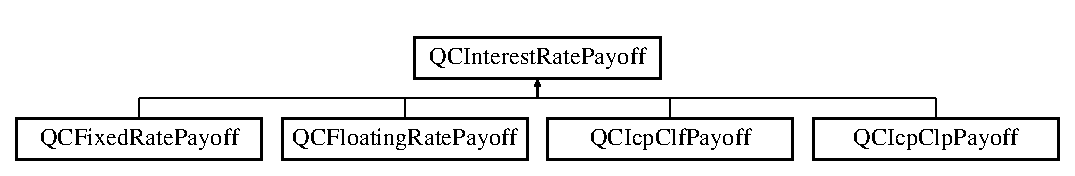
\includegraphics[height=1.917808cm]{class_q_c_interest_rate_payoff}
\end{center}
\end{figure}
\subsection*{Public Member Functions}
\begin{DoxyCompactItemize}
\item 
void \hyperlink{class_q_c_interest_rate_payoff_a3e218905ae425cad5283b438d338becc}{payoff} ()
\item 
int \hyperlink{class_q_c_interest_rate_payoff_a9277006372cd491323a9e4dce6d3cb85}{payoff\+Size} ()
\item 
double \hyperlink{class_q_c_interest_rate_payoff_a07a3040226a9996e4e77b4a39e3dbb31}{get\+Value\+Date\+Cashflow} ()
\item 
double \hyperlink{class_q_c_interest_rate_payoff_aa1fa4acff91e83dfb2174a4067c0231f}{present\+Value} ()
\item 
double \hyperlink{class_q_c_interest_rate_payoff_a1f1b38019791d59e4fd4053652da72a4}{get\+Pv\+Rate\+Derivative\+At} (unsigned int index)
\item 
double \hyperlink{class_q_c_interest_rate_payoff_a4c6072e011a2a05bcf45b2dbdfe33d56}{get\+Pv\+Proj\+Rate\+Derivative\+At} (unsigned int index)
\item 
unsigned long \hyperlink{class_q_c_interest_rate_payoff_ab2b6f0b4059cd77feb33d8d153a6366c}{discount\+Curve\+Length} ()
\item 
unsigned long \hyperlink{class_q_c_interest_rate_payoff_a15936bf1fd9af7d442393efc681e4f63}{projecting\+Curve\+Length} ()
\item 
tuple$<$ \hyperlink{class_q_c_date}{Q\+C\+Date}, Q\+C\+Cash\+Flow\+Label, \\*
double $>$ \hyperlink{class_q_c_interest_rate_payoff_a5c696c809dddf2c442f2aa25cfe7b55d}{get\+Cashflow\+At} (unsigned int n)
\item 
virtual \hyperlink{class_q_c_interest_rate_payoff_ae446121666d1b9b0573322977a2a907a}{$\sim$\+Q\+C\+Interest\+Rate\+Payoff} ()
\end{DoxyCompactItemize}
\subsection*{Protected Member Functions}
\begin{DoxyCompactItemize}
\item 
\hypertarget{class_q_c_interest_rate_payoff_a3ef90fad027f853c7d70ad3ae609edc6}{{\bfseries Q\+C\+Interest\+Rate\+Payoff} (\hyperlink{_q_c_definitions_8h_ae6a21ad26d19e482e3b01179cbc05298}{Q\+C\+Intrst\+Rt\+Shrd\+Ptr} rate, shared\+\_\+ptr$<$ \hyperlink{class_q_c_interest_rate_leg}{Q\+C\+Interest\+Rate\+Leg} $>$ ir\+Leg, \hyperlink{class_q_c_date}{Q\+C\+Date} value\+Date, \hyperlink{_q_c_definitions_8h_a4b4fb466e49550e3dfd40003562cd19d}{Q\+C\+Int\+Rt\+Crv\+Shrd\+Ptr} projecting\+Curve, \hyperlink{_q_c_definitions_8h_a4b4fb466e49550e3dfd40003562cd19d}{Q\+C\+Int\+Rt\+Crv\+Shrd\+Ptr} discount\+Curve, \hyperlink{_q_c_definitions_8h_a6a601ffd693c05dd81309e3dca08b8f5}{Q\+C\+Time\+Series\+Shrd\+Ptr} fixing\+Data)}\label{class_q_c_interest_rate_payoff_a3ef90fad027f853c7d70ad3ae609edc6}

\item 
\hypertarget{class_q_c_interest_rate_payoff_aae61a0e8b38e909f31b6b170a5785748}{virtual void {\bfseries \+\_\+set\+All\+Rates} ()}\label{class_q_c_interest_rate_payoff_aae61a0e8b38e909f31b6b170a5785748}

\end{DoxyCompactItemize}
\subsection*{Protected Attributes}
\begin{DoxyCompactItemize}
\item 
\hypertarget{class_q_c_interest_rate_payoff_a60cda238d4546b03aa286fe46b8da62c}{\hyperlink{_q_c_definitions_8h_ae6a21ad26d19e482e3b01179cbc05298}{Q\+C\+Intrst\+Rt\+Shrd\+Ptr} {\bfseries \+\_\+rate}}\label{class_q_c_interest_rate_payoff_a60cda238d4546b03aa286fe46b8da62c}

\item 
\hypertarget{class_q_c_interest_rate_payoff_a1b2b849d61696578c7d06d71b5c4c6f4}{shared\+\_\+ptr$<$ \hyperlink{class_q_c_interest_rate_leg}{Q\+C\+Interest\+Rate\+Leg} $>$ {\bfseries \+\_\+ir\+Leg}}\label{class_q_c_interest_rate_payoff_a1b2b849d61696578c7d06d71b5c4c6f4}

\item 
\hypertarget{class_q_c_interest_rate_payoff_a6bab476f9fb3c09af76311ffebf245e8}{\hyperlink{class_q_c_date}{Q\+C\+Date} {\bfseries \+\_\+value\+Date}}\label{class_q_c_interest_rate_payoff_a6bab476f9fb3c09af76311ffebf245e8}

\item 
\hypertarget{class_q_c_interest_rate_payoff_a8849771f1a8bc47a024db46d11bc1244}{\hyperlink{_q_c_definitions_8h_a4b4fb466e49550e3dfd40003562cd19d}{Q\+C\+Int\+Rt\+Crv\+Shrd\+Ptr} {\bfseries \+\_\+projecting\+Curve}}\label{class_q_c_interest_rate_payoff_a8849771f1a8bc47a024db46d11bc1244}

\item 
\hypertarget{class_q_c_interest_rate_payoff_a74dc75796c398ab2878b8b4e48fa81c4}{\hyperlink{_q_c_definitions_8h_a4b4fb466e49550e3dfd40003562cd19d}{Q\+C\+Int\+Rt\+Crv\+Shrd\+Ptr} {\bfseries \+\_\+discount\+Curve}}\label{class_q_c_interest_rate_payoff_a74dc75796c398ab2878b8b4e48fa81c4}

\item 
\hypertarget{class_q_c_interest_rate_payoff_a00403e0cfa9b5e4d050921e7ef3fcb7b}{\hyperlink{_q_c_definitions_8h_a6a601ffd693c05dd81309e3dca08b8f5}{Q\+C\+Time\+Series\+Shrd\+Ptr} {\bfseries \+\_\+fixing\+Data}}\label{class_q_c_interest_rate_payoff_a00403e0cfa9b5e4d050921e7ef3fcb7b}

\item 
\hypertarget{class_q_c_interest_rate_payoff_acbed42b93a13fb7346e0390ad83acafd}{int {\bfseries \+\_\+current\+Period}}\label{class_q_c_interest_rate_payoff_acbed42b93a13fb7346e0390ad83acafd}

\item 
\hypertarget{class_q_c_interest_rate_payoff_a29527bbc61ba81fa84e9978f7fd94edb}{vector$<$ tuple$<$ \hyperlink{class_q_c_date}{Q\+C\+Date}, \\*
Q\+C\+Cash\+Flow\+Label, double $>$ $>$ {\bfseries \+\_\+payoffs}}\label{class_q_c_interest_rate_payoff_a29527bbc61ba81fa84e9978f7fd94edb}

\item 
\hypertarget{class_q_c_interest_rate_payoff_a0055baa42a22388a201534c188403d07}{vector$<$ double $>$ {\bfseries \+\_\+all\+Rates}}\label{class_q_c_interest_rate_payoff_a0055baa42a22388a201534c188403d07}

\item 
\hypertarget{class_q_c_interest_rate_payoff_a832d4808ce5a927c22096dcf9c699c47}{double {\bfseries \+\_\+value\+Date\+Cashflow}}\label{class_q_c_interest_rate_payoff_a832d4808ce5a927c22096dcf9c699c47}

\item 
\hypertarget{class_q_c_interest_rate_payoff_a3016cee34dde022c62757714d9dc3431}{vector$<$ double $>$ {\bfseries \+\_\+pv\+Rate\+Derivatives}}\label{class_q_c_interest_rate_payoff_a3016cee34dde022c62757714d9dc3431}

\item 
\hypertarget{class_q_c_interest_rate_payoff_ae167b48aed467caa1ddc1392b21bc44d}{vector$<$ vector$<$ double $>$ $>$ {\bfseries \+\_\+all\+Rates\+Derivatives}}\label{class_q_c_interest_rate_payoff_ae167b48aed467caa1ddc1392b21bc44d}

\item 
\hypertarget{class_q_c_interest_rate_payoff_a4b8d7f37769cfb641ec55e06dd60f24d}{vector$<$ double $>$ {\bfseries \+\_\+pv\+Proj\+Curve\+Derivatives}}\label{class_q_c_interest_rate_payoff_a4b8d7f37769cfb641ec55e06dd60f24d}

\end{DoxyCompactItemize}


\subsection{Detailed Description}


Definition at line 21 of file Q\+C\+Interest\+Rate\+Payoff.\+h.



\subsection{Constructor \& Destructor Documentation}
\hypertarget{class_q_c_interest_rate_payoff_ae446121666d1b9b0573322977a2a907a}{\index{Q\+C\+Interest\+Rate\+Payoff@{Q\+C\+Interest\+Rate\+Payoff}!````~Q\+C\+Interest\+Rate\+Payoff@{$\sim$\+Q\+C\+Interest\+Rate\+Payoff}}
\index{````~Q\+C\+Interest\+Rate\+Payoff@{$\sim$\+Q\+C\+Interest\+Rate\+Payoff}!Q\+C\+Interest\+Rate\+Payoff@{Q\+C\+Interest\+Rate\+Payoff}}
\subsubsection[{$\sim$\+Q\+C\+Interest\+Rate\+Payoff}]{\setlength{\rightskip}{0pt plus 5cm}virtual Q\+C\+Interest\+Rate\+Payoff\+::$\sim$\+Q\+C\+Interest\+Rate\+Payoff (
\begin{DoxyParamCaption}
{}
\end{DoxyParamCaption}
)\hspace{0.3cm}{\ttfamily [virtual]}}}\label{class_q_c_interest_rate_payoff_ae446121666d1b9b0573322977a2a907a}
Destructor 

\subsection{Member Function Documentation}
\hypertarget{class_q_c_interest_rate_payoff_ab2b6f0b4059cd77feb33d8d153a6366c}{\index{Q\+C\+Interest\+Rate\+Payoff@{Q\+C\+Interest\+Rate\+Payoff}!discount\+Curve\+Length@{discount\+Curve\+Length}}
\index{discount\+Curve\+Length@{discount\+Curve\+Length}!Q\+C\+Interest\+Rate\+Payoff@{Q\+C\+Interest\+Rate\+Payoff}}
\subsubsection[{discount\+Curve\+Length}]{\setlength{\rightskip}{0pt plus 5cm}unsigned long Q\+C\+Interest\+Rate\+Payoff\+::discount\+Curve\+Length (
\begin{DoxyParamCaption}
{}
\end{DoxyParamCaption}
)}}\label{class_q_c_interest_rate_payoff_ab2b6f0b4059cd77feb33d8d153a6366c}
Retorna el largo (numero de vertices) de la curva de descuento. \begin{DoxyReturn}{Returns}
(unsigned long) largo de la curva. 
\end{DoxyReturn}
\hypertarget{class_q_c_interest_rate_payoff_a5c696c809dddf2c442f2aa25cfe7b55d}{\index{Q\+C\+Interest\+Rate\+Payoff@{Q\+C\+Interest\+Rate\+Payoff}!get\+Cashflow\+At@{get\+Cashflow\+At}}
\index{get\+Cashflow\+At@{get\+Cashflow\+At}!Q\+C\+Interest\+Rate\+Payoff@{Q\+C\+Interest\+Rate\+Payoff}}
\subsubsection[{get\+Cashflow\+At}]{\setlength{\rightskip}{0pt plus 5cm}tuple$<${\bf Q\+C\+Date}, Q\+C\+Cash\+Flow\+Label, double$>$ Q\+C\+Interest\+Rate\+Payoff\+::get\+Cashflow\+At (
\begin{DoxyParamCaption}
\item[{unsigned int}]{n}
\end{DoxyParamCaption}
)}}\label{class_q_c_interest_rate_payoff_a5c696c809dddf2c442f2aa25cfe7b55d}
Retorna la tupla que describe el cashflow en el indice n del vector donde se registran los cashflows del payoff. Cada cashflow se forma con una fecha (fecha del cashflow), una etiqueta que indica que tipo de casflow es (interes, disposicion o amortizacion) y el monto del cashflow. 
\begin{DoxyParams}{Parameters}
{\em n} & indice del cashflow solicitado. \\
\hline
\end{DoxyParams}
\begin{DoxyReturn}{Returns}
(tuple$<$\+Q\+C\+Date, Q\+C\+Cash\+Flow\+Label, double$>$) cashflow. 
\end{DoxyReturn}
\hypertarget{class_q_c_interest_rate_payoff_a4c6072e011a2a05bcf45b2dbdfe33d56}{\index{Q\+C\+Interest\+Rate\+Payoff@{Q\+C\+Interest\+Rate\+Payoff}!get\+Pv\+Proj\+Rate\+Derivative\+At@{get\+Pv\+Proj\+Rate\+Derivative\+At}}
\index{get\+Pv\+Proj\+Rate\+Derivative\+At@{get\+Pv\+Proj\+Rate\+Derivative\+At}!Q\+C\+Interest\+Rate\+Payoff@{Q\+C\+Interest\+Rate\+Payoff}}
\subsubsection[{get\+Pv\+Proj\+Rate\+Derivative\+At}]{\setlength{\rightskip}{0pt plus 5cm}double Q\+C\+Interest\+Rate\+Payoff\+::get\+Pv\+Proj\+Rate\+Derivative\+At (
\begin{DoxyParamCaption}
\item[{unsigned int}]{index}
\end{DoxyParamCaption}
)}}\label{class_q_c_interest_rate_payoff_a4c6072e011a2a05bcf45b2dbdfe33d56}
Retorna la derivada del valor presente respecto a la componente index de la curva de proyeccion (se cuenta a partir de 0). 
\begin{DoxyParams}{Parameters}
{\em index} & el indice solicitado \\
\hline
\end{DoxyParams}
\begin{DoxyReturn}{Returns}
(double) la derivada solicitada 
\end{DoxyReturn}
\hypertarget{class_q_c_interest_rate_payoff_a1f1b38019791d59e4fd4053652da72a4}{\index{Q\+C\+Interest\+Rate\+Payoff@{Q\+C\+Interest\+Rate\+Payoff}!get\+Pv\+Rate\+Derivative\+At@{get\+Pv\+Rate\+Derivative\+At}}
\index{get\+Pv\+Rate\+Derivative\+At@{get\+Pv\+Rate\+Derivative\+At}!Q\+C\+Interest\+Rate\+Payoff@{Q\+C\+Interest\+Rate\+Payoff}}
\subsubsection[{get\+Pv\+Rate\+Derivative\+At}]{\setlength{\rightskip}{0pt plus 5cm}double Q\+C\+Interest\+Rate\+Payoff\+::get\+Pv\+Rate\+Derivative\+At (
\begin{DoxyParamCaption}
\item[{unsigned int}]{index}
\end{DoxyParamCaption}
)}}\label{class_q_c_interest_rate_payoff_a1f1b38019791d59e4fd4053652da72a4}
Retorna la derivada del valor presente respecto a la componente index de la curva de descuento (se cuenta a partir de 0). 
\begin{DoxyParams}{Parameters}
{\em index} & el indice solicitado \\
\hline
\end{DoxyParams}
\begin{DoxyReturn}{Returns}
(double) la derivada solicitada 
\end{DoxyReturn}
\hypertarget{class_q_c_interest_rate_payoff_a07a3040226a9996e4e77b4a39e3dbb31}{\index{Q\+C\+Interest\+Rate\+Payoff@{Q\+C\+Interest\+Rate\+Payoff}!get\+Value\+Date\+Cashflow@{get\+Value\+Date\+Cashflow}}
\index{get\+Value\+Date\+Cashflow@{get\+Value\+Date\+Cashflow}!Q\+C\+Interest\+Rate\+Payoff@{Q\+C\+Interest\+Rate\+Payoff}}
\subsubsection[{get\+Value\+Date\+Cashflow}]{\setlength{\rightskip}{0pt plus 5cm}double Q\+C\+Interest\+Rate\+Payoff\+::get\+Value\+Date\+Cashflow (
\begin{DoxyParamCaption}
{}
\end{DoxyParamCaption}
)}}\label{class_q_c_interest_rate_payoff_a07a3040226a9996e4e77b4a39e3dbb31}
Retorna el valor del flujo de caja de \+\_\+value\+Date \begin{DoxyReturn}{Returns}
(double) el valor del cashflow 
\end{DoxyReturn}
\hypertarget{class_q_c_interest_rate_payoff_a3e218905ae425cad5283b438d338becc}{\index{Q\+C\+Interest\+Rate\+Payoff@{Q\+C\+Interest\+Rate\+Payoff}!payoff@{payoff}}
\index{payoff@{payoff}!Q\+C\+Interest\+Rate\+Payoff@{Q\+C\+Interest\+Rate\+Payoff}}
\subsubsection[{payoff}]{\setlength{\rightskip}{0pt plus 5cm}void Q\+C\+Interest\+Rate\+Payoff\+::payoff (
\begin{DoxyParamCaption}
{}
\end{DoxyParamCaption}
)}}\label{class_q_c_interest_rate_payoff_a3e218905ae425cad5283b438d338becc}
Genera los flujos de caja y los guarda dentro de la clase \begin{DoxyReturn}{Returns}
(void) 
\end{DoxyReturn}
\hypertarget{class_q_c_interest_rate_payoff_a9277006372cd491323a9e4dce6d3cb85}{\index{Q\+C\+Interest\+Rate\+Payoff@{Q\+C\+Interest\+Rate\+Payoff}!payoff\+Size@{payoff\+Size}}
\index{payoff\+Size@{payoff\+Size}!Q\+C\+Interest\+Rate\+Payoff@{Q\+C\+Interest\+Rate\+Payoff}}
\subsubsection[{payoff\+Size}]{\setlength{\rightskip}{0pt plus 5cm}int Q\+C\+Interest\+Rate\+Payoff\+::payoff\+Size (
\begin{DoxyParamCaption}
{}
\end{DoxyParamCaption}
)}}\label{class_q_c_interest_rate_payoff_a9277006372cd491323a9e4dce6d3cb85}
Calcula y retorna el numero de flujos de caja \begin{DoxyReturn}{Returns}
(int) el numero de flujos 
\end{DoxyReturn}
\hypertarget{class_q_c_interest_rate_payoff_aa1fa4acff91e83dfb2174a4067c0231f}{\index{Q\+C\+Interest\+Rate\+Payoff@{Q\+C\+Interest\+Rate\+Payoff}!present\+Value@{present\+Value}}
\index{present\+Value@{present\+Value}!Q\+C\+Interest\+Rate\+Payoff@{Q\+C\+Interest\+Rate\+Payoff}}
\subsubsection[{present\+Value}]{\setlength{\rightskip}{0pt plus 5cm}double Q\+C\+Interest\+Rate\+Payoff\+::present\+Value (
\begin{DoxyParamCaption}
{}
\end{DoxyParamCaption}
)}}\label{class_q_c_interest_rate_payoff_aa1fa4acff91e83dfb2174a4067c0231f}
Calcula y retorna el valor presente de la pata descontando con la curva de descuento. Dentro de este proceso se calculan tambien las derivadas del valor presente respecto a cada punto de las curvas de descuento y proyeccion. \begin{DoxyReturn}{Returns}
(double) el valor presente 
\end{DoxyReturn}
\hypertarget{class_q_c_interest_rate_payoff_a15936bf1fd9af7d442393efc681e4f63}{\index{Q\+C\+Interest\+Rate\+Payoff@{Q\+C\+Interest\+Rate\+Payoff}!projecting\+Curve\+Length@{projecting\+Curve\+Length}}
\index{projecting\+Curve\+Length@{projecting\+Curve\+Length}!Q\+C\+Interest\+Rate\+Payoff@{Q\+C\+Interest\+Rate\+Payoff}}
\subsubsection[{projecting\+Curve\+Length}]{\setlength{\rightskip}{0pt plus 5cm}unsigned long Q\+C\+Interest\+Rate\+Payoff\+::projecting\+Curve\+Length (
\begin{DoxyParamCaption}
{}
\end{DoxyParamCaption}
)}}\label{class_q_c_interest_rate_payoff_a15936bf1fd9af7d442393efc681e4f63}
Retorna el largo (numero de vertices) de la curva de proyeccion. \begin{DoxyReturn}{Returns}
(unsigned long) largo de la curva. 
\end{DoxyReturn}


The documentation for this class was generated from the following file\+:\begin{DoxyCompactItemize}
\item 
include/Q\+C\+Interest\+Rate\+Payoff.\+h\end{DoxyCompactItemize}

\hypertarget{class_q_c_interest_rate_periods_factory}{\section{Q\+C\+Interest\+Rate\+Periods\+Factory Class Reference}
\label{class_q_c_interest_rate_periods_factory}\index{Q\+C\+Interest\+Rate\+Periods\+Factory@{Q\+C\+Interest\+Rate\+Periods\+Factory}}
}
\subsection*{Public Member Functions}
\begin{DoxyCompactItemize}
\item 
\hypertarget{class_q_c_interest_rate_periods_factory_a5421afc68914df1c7aa9310c79466336}{{\bfseries Q\+C\+Interest\+Rate\+Periods\+Factory} (\hyperlink{class_q_c_date}{Q\+C\+Date} start\+Date, \hyperlink{class_q_c_date}{Q\+C\+Date} end\+Date, \hyperlink{class_q_c_date_a17e5b6c9a1a784f917c8e84045d7e362}{Q\+C\+Date\+::\+Q\+C\+Bus\+Day\+Adj\+Rules} end\+Date\+Adjustment, string settlement\+Periodicity, \hyperlink{class_q_c_interest_rate_leg_a70e636ef79eb9bc4c6b84ea526e56521}{Q\+C\+Interest\+Rate\+Leg\+::\+Q\+C\+Stub\+Period} settlement\+Stub\+Period, shared\+\_\+ptr$<$ vector$<$ \hyperlink{class_q_c_date}{Q\+C\+Date} $>$$>$ settlement\+Calendar, unsigned int settlement\+Lag, string fixing\+Periodicity, \hyperlink{class_q_c_interest_rate_leg_a70e636ef79eb9bc4c6b84ea526e56521}{Q\+C\+Interest\+Rate\+Leg\+::\+Q\+C\+Stub\+Period} fixing\+Stub\+Period, shared\+\_\+ptr$<$ vector$<$ \hyperlink{class_q_c_date}{Q\+C\+Date} $>$$>$ fixing\+Calendar, unsigned int fixing\+Lag, unsigned int index\+Start\+Date\+Lag, string index\+Tenor)}\label{class_q_c_interest_rate_periods_factory_a5421afc68914df1c7aa9310c79466336}

\item 
\hypertarget{class_q_c_interest_rate_periods_factory_a95073c612b862bbd84e00048f93338a7}{\hyperlink{class_q_c_interest_rate_leg_ad04f1da06a7b5d44fea906bd8c62de28}{Q\+C\+Interest\+Rate\+Leg\+::\+Q\+C\+Interest\+Rate\+Periods} {\bfseries get\+Periods} ()}\label{class_q_c_interest_rate_periods_factory_a95073c612b862bbd84e00048f93338a7}

\end{DoxyCompactItemize}


\subsection{Detailed Description}


Definition at line 12 of file Q\+C\+Interest\+Rate\+Periods\+Factory.\+h.



The documentation for this class was generated from the following file\+:\begin{DoxyCompactItemize}
\item 
include/Q\+C\+Interest\+Rate\+Periods\+Factory.\+h\end{DoxyCompactItemize}

\hypertarget{class_q_c_interpolator}{\section{Q\+C\+Interpolator Class Reference}
\label{class_q_c_interpolator}\index{Q\+C\+Interpolator@{Q\+C\+Interpolator}}
}
Inheritance diagram for Q\+C\+Interpolator\+:\begin{figure}[H]
\begin{center}
\leavevmode
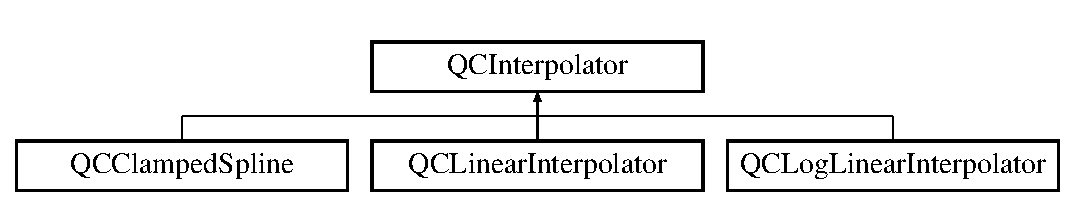
\includegraphics[height=2.000000cm]{class_q_c_interpolator}
\end{center}
\end{figure}
\subsection*{Public Member Functions}
\begin{DoxyCompactItemize}
\item 
\hypertarget{class_q_c_interpolator_a403ed055096d89353b00a6ab32a18f05}{{\bfseries Q\+C\+Interpolator} (shared\+\_\+ptr$<$ \hyperlink{class_q_c_curve}{Q\+C\+Curve}$<$ long $>$$>$ curve)}\label{class_q_c_interpolator_a403ed055096d89353b00a6ab32a18f05}

\item 
\hypertarget{class_q_c_interpolator_a79b39c3c85d42d87faa938a3dc55b37d}{virtual double {\bfseries interpolate\+At} (long value)}\label{class_q_c_interpolator_a79b39c3c85d42d87faa938a3dc55b37d}

\item 
\hypertarget{class_q_c_interpolator_a8c00193c882786d6592979c87aaf1d15}{virtual double {\bfseries derivative\+At} (long value)}\label{class_q_c_interpolator_a8c00193c882786d6592979c87aaf1d15}

\item 
\hypertarget{class_q_c_interpolator_a9b258b5354f6dac04ce65a1f97874261}{virtual double {\bfseries second\+Derivative\+At} (long value)}\label{class_q_c_interpolator_a9b258b5354f6dac04ce65a1f97874261}

\item 
\hypertarget{class_q_c_interpolator_afc9bf8b0d87050efca3a6633c121580f}{double {\bfseries rate\+Derivative\+At} (unsigned int rate\+Index)}\label{class_q_c_interpolator_afc9bf8b0d87050efca3a6633c121580f}

\item 
\hypertarget{class_q_c_interpolator_a0830d56af8995cdb04a437b0e36fa44a}{long {\bfseries get\+Length} ()}\label{class_q_c_interpolator_a0830d56af8995cdb04a437b0e36fa44a}

\end{DoxyCompactItemize}
\subsection*{Protected Member Functions}
\begin{DoxyCompactItemize}
\item 
\hypertarget{class_q_c_interpolator_a72bf1a0bb40df70d4b90e2a6d8c032f8}{long {\bfseries index} (long arg)}\label{class_q_c_interpolator_a72bf1a0bb40df70d4b90e2a6d8c032f8}

\end{DoxyCompactItemize}
\subsection*{Protected Attributes}
\begin{DoxyCompactItemize}
\item 
\hypertarget{class_q_c_interpolator_ade6d623eb8e1a40b0337d41f511781dd}{shared\+\_\+ptr$<$ \hyperlink{class_q_c_curve}{Q\+C\+Curve}$<$ long $>$ $>$ {\bfseries \+\_\+curve}}\label{class_q_c_interpolator_ade6d623eb8e1a40b0337d41f511781dd}

\item 
\hypertarget{class_q_c_interpolator_ac16264cdb256f83cc64d40719c2658c1}{vector$<$ double $>$ {\bfseries \+\_\+derivatives}}\label{class_q_c_interpolator_ac16264cdb256f83cc64d40719c2658c1}

\end{DoxyCompactItemize}


\subsection{Detailed Description}


Definition at line 9 of file Q\+C\+Interpolator.\+h.



The documentation for this class was generated from the following file\+:\begin{DoxyCompactItemize}
\item 
include/Q\+C\+Interpolator.\+h\end{DoxyCompactItemize}

\hypertarget{class_q_c_linear_interpolator}{\section{Q\+C\+Linear\+Interpolator Class Reference}
\label{class_q_c_linear_interpolator}\index{Q\+C\+Linear\+Interpolator@{Q\+C\+Linear\+Interpolator}}
}
Inheritance diagram for Q\+C\+Linear\+Interpolator\+:\begin{figure}[H]
\begin{center}
\leavevmode
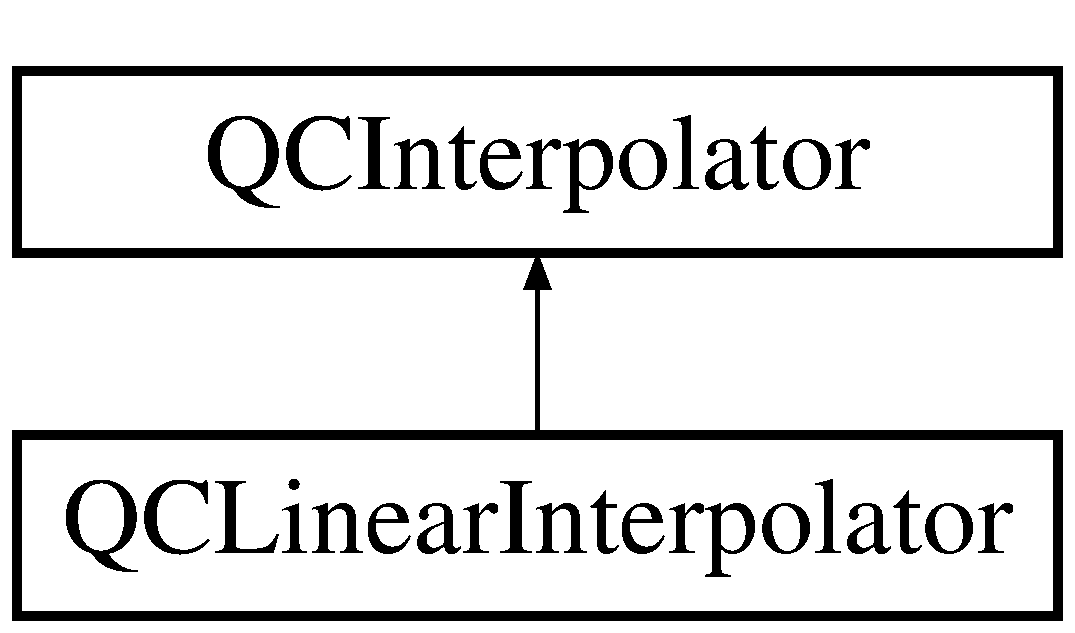
\includegraphics[height=2.000000cm]{class_q_c_linear_interpolator}
\end{center}
\end{figure}
\subsection*{Public Member Functions}
\begin{DoxyCompactItemize}
\item 
\hypertarget{class_q_c_linear_interpolator_afa1b20df27939e047743dda0a9c34ca1}{{\bfseries Q\+C\+Linear\+Interpolator} (shared\+\_\+ptr$<$ \hyperlink{class_q_c_curve}{Q\+C\+Curve}$<$ long $>$$>$ curve)}\label{class_q_c_linear_interpolator_afa1b20df27939e047743dda0a9c34ca1}

\item 
\hypertarget{class_q_c_linear_interpolator_a6eb1ce1cd8f7acba77bca9b095ada4e2}{virtual double {\bfseries interpolate\+At} (long value) override}\label{class_q_c_linear_interpolator_a6eb1ce1cd8f7acba77bca9b095ada4e2}

\item 
\hypertarget{class_q_c_linear_interpolator_a1935db5d0b62bbfc99cb9cf3200a2305}{virtual double {\bfseries derivative\+At} (long value) override}\label{class_q_c_linear_interpolator_a1935db5d0b62bbfc99cb9cf3200a2305}

\item 
\hypertarget{class_q_c_linear_interpolator_a222277421d69de76c97a6011e72b84b4}{virtual double {\bfseries second\+Derivative\+At} (long value) override}\label{class_q_c_linear_interpolator_a222277421d69de76c97a6011e72b84b4}

\end{DoxyCompactItemize}
\subsection*{Additional Inherited Members}


\subsection{Detailed Description}


Definition at line 6 of file Q\+C\+Linear\+Interpolator.\+h.



The documentation for this class was generated from the following file\+:\begin{DoxyCompactItemize}
\item 
include/Q\+C\+Linear\+Interpolator.\+h\end{DoxyCompactItemize}

\hypertarget{class_q_c_linear_wf}{\section{Q\+C\+Linear\+Wf Class Reference}
\label{class_q_c_linear_wf}\index{Q\+C\+Linear\+Wf@{Q\+C\+Linear\+Wf}}
}
Inheritance diagram for Q\+C\+Linear\+Wf\+:\begin{figure}[H]
\begin{center}
\leavevmode
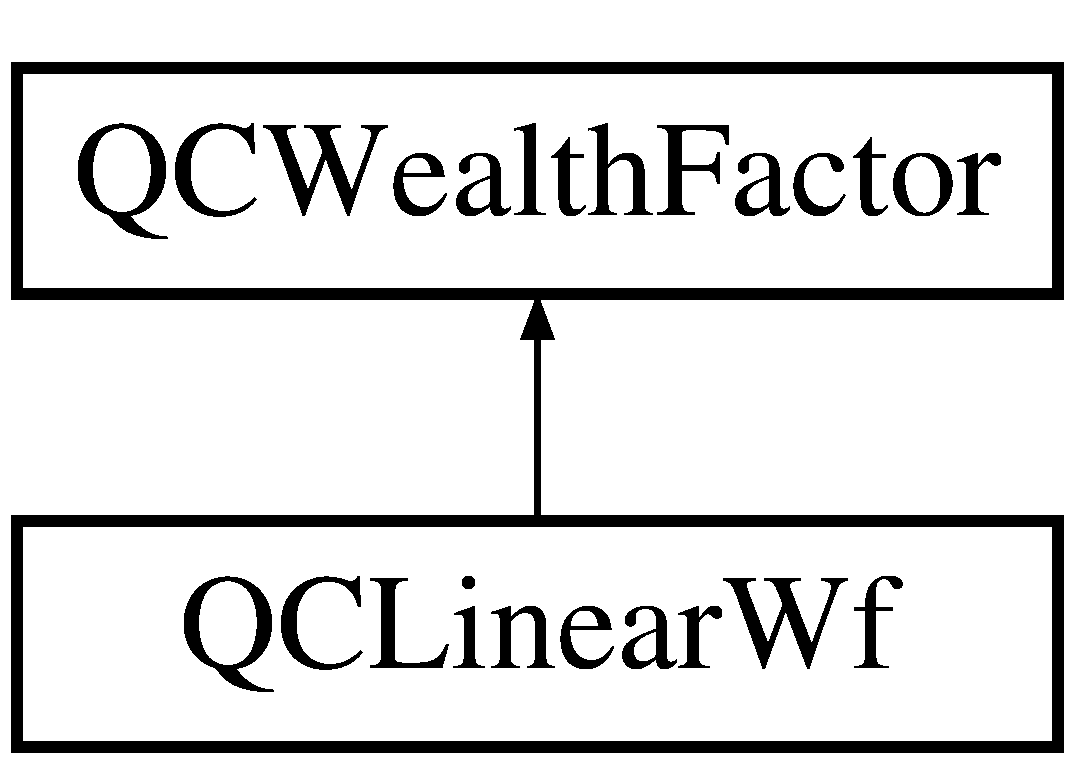
\includegraphics[height=2.000000cm]{class_q_c_linear_wf}
\end{center}
\end{figure}
\subsection*{Public Member Functions}
\begin{DoxyCompactItemize}
\item 
virtual double \hyperlink{class_q_c_linear_wf_ad9ac92ae46857a060f47ceda4291bd72}{wf} (double \hyperlink{class_q_c_linear_wf_ad0a049fd92a36cecd4b766b181a3cf7b}{rate}, double yf) override
\item 
virtual double \hyperlink{class_q_c_linear_wf_ad0a049fd92a36cecd4b766b181a3cf7b}{rate} (double \hyperlink{class_q_c_linear_wf_ad9ac92ae46857a060f47ceda4291bd72}{wf}, double yf) override
\end{DoxyCompactItemize}
\subsection*{Additional Inherited Members}


\subsection{Detailed Description}


Definition at line 6 of file Q\+C\+Linear\+Wf.\+h.



\subsection{Member Function Documentation}
\hypertarget{class_q_c_linear_wf_ad0a049fd92a36cecd4b766b181a3cf7b}{\index{Q\+C\+Linear\+Wf@{Q\+C\+Linear\+Wf}!rate@{rate}}
\index{rate@{rate}!Q\+C\+Linear\+Wf@{Q\+C\+Linear\+Wf}}
\subsubsection[{rate}]{\setlength{\rightskip}{0pt plus 5cm}virtual double Q\+C\+Linear\+Wf\+::rate (
\begin{DoxyParamCaption}
\item[{double}]{wf, }
\item[{double}]{yf}
\end{DoxyParamCaption}
)\hspace{0.3cm}{\ttfamily [override]}, {\ttfamily [virtual]}}}\label{class_q_c_linear_wf_ad0a049fd92a36cecd4b766b181a3cf7b}
La función rate devuelve el valor de la tasa asociada al valor del factor de capitalización y su fracción de año asociada. 
\begin{DoxyParams}{Parameters}
{\em wf} & es el valor del factor de capitalización \\
\hline
{\em yf} & es el valor de la fracción de año \\
\hline
\end{DoxyParams}
\begin{DoxyReturn}{Returns}
(double) valor de la tasa asociada 
\end{DoxyReturn}


Implements \hyperlink{class_q_c_wealth_factor_aad4a3d84f0c2073162cc5fcce5509d1c}{Q\+C\+Wealth\+Factor}.

\hypertarget{class_q_c_linear_wf_ad9ac92ae46857a060f47ceda4291bd72}{\index{Q\+C\+Linear\+Wf@{Q\+C\+Linear\+Wf}!wf@{wf}}
\index{wf@{wf}!Q\+C\+Linear\+Wf@{Q\+C\+Linear\+Wf}}
\subsubsection[{wf}]{\setlength{\rightskip}{0pt plus 5cm}virtual double Q\+C\+Linear\+Wf\+::wf (
\begin{DoxyParamCaption}
\item[{double}]{rate, }
\item[{double}]{yf}
\end{DoxyParamCaption}
)\hspace{0.3cm}{\ttfamily [override]}, {\ttfamily [virtual]}}}\label{class_q_c_linear_wf_ad9ac92ae46857a060f47ceda4291bd72}
La función wf devuelve el valor del factor de capitalización dado el valor de una tasa y su fracción de año asociada. Cuando se invoca este método, también se calcula la derivada del factor de capitalización respecto al parámetro rate. Este valor se almacena en la variable protected \+\_\+dwf 
\begin{DoxyParams}{Parameters}
{\em rate} & es el valor de la tasa \\
\hline
{\em yf} & es el valor de la fracción de año \\
\hline
\end{DoxyParams}
\begin{DoxyReturn}{Returns}
(double) valor del factor de capitalización 
\end{DoxyReturn}


Implements \hyperlink{class_q_c_wealth_factor_a63ddc9c957aa438c1278b541f6e1ebbe}{Q\+C\+Wealth\+Factor}.



The documentation for this class was generated from the following file\+:\begin{DoxyCompactItemize}
\item 
include/Q\+C\+Linear\+Wf.\+h\end{DoxyCompactItemize}

\hypertarget{class_q_c_log_linear_interpolator}{\section{Q\+C\+Log\+Linear\+Interpolator Class Reference}
\label{class_q_c_log_linear_interpolator}\index{Q\+C\+Log\+Linear\+Interpolator@{Q\+C\+Log\+Linear\+Interpolator}}
}
Inheritance diagram for Q\+C\+Log\+Linear\+Interpolator\+:\begin{figure}[H]
\begin{center}
\leavevmode
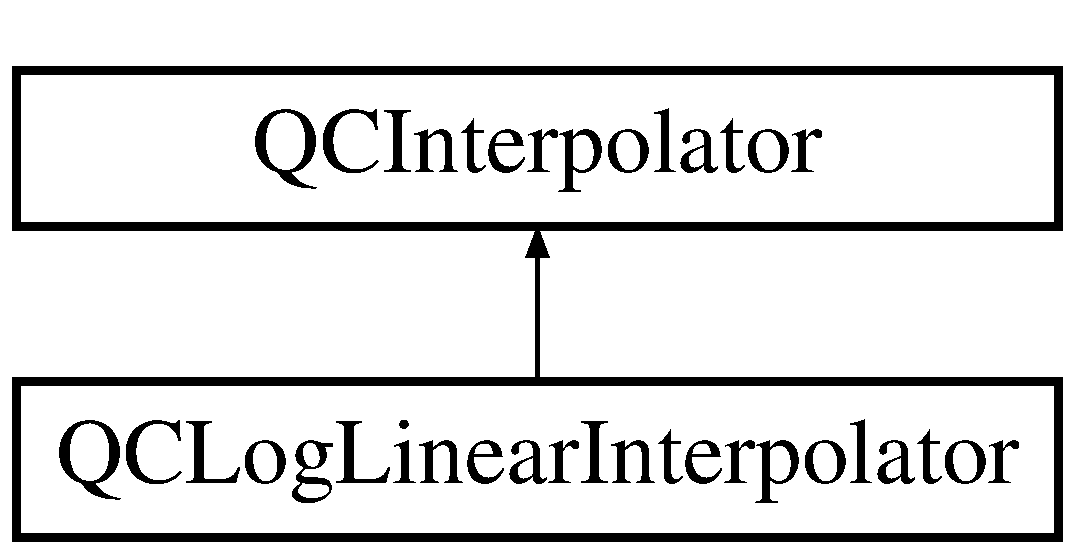
\includegraphics[height=2.000000cm]{class_q_c_log_linear_interpolator}
\end{center}
\end{figure}
\subsection*{Public Member Functions}
\begin{DoxyCompactItemize}
\item 
\hypertarget{class_q_c_log_linear_interpolator_a498be15254b804596bd1c8e3ef09efe5}{{\bfseries Q\+C\+Log\+Linear\+Interpolator} (shared\+\_\+ptr$<$ \hyperlink{class_q_c_curve}{Q\+C\+Curve}$<$ long $>$$>$ curve)}\label{class_q_c_log_linear_interpolator_a498be15254b804596bd1c8e3ef09efe5}

\item 
\hypertarget{class_q_c_log_linear_interpolator_aa19f97d5e9945707ea736557d24848c2}{virtual double {\bfseries interpolate\+At} (long value) override}\label{class_q_c_log_linear_interpolator_aa19f97d5e9945707ea736557d24848c2}

\item 
\hypertarget{class_q_c_log_linear_interpolator_a6eab6867f1f9bfe8efc9a0f43b8d4e08}{virtual double {\bfseries derivative\+At} (long value) override}\label{class_q_c_log_linear_interpolator_a6eab6867f1f9bfe8efc9a0f43b8d4e08}

\item 
\hypertarget{class_q_c_log_linear_interpolator_a5fd88a365a48f63d0a644677a12abf3f}{virtual double {\bfseries second\+Derivative\+At} (long value) override}\label{class_q_c_log_linear_interpolator_a5fd88a365a48f63d0a644677a12abf3f}

\end{DoxyCompactItemize}
\subsection*{Additional Inherited Members}


\subsection{Detailed Description}


Definition at line 6 of file Q\+C\+Log\+Linear\+Interpolator.\+h.



The documentation for this class was generated from the following file\+:\begin{DoxyCompactItemize}
\item 
include/Q\+C\+Log\+Linear\+Interpolator.\+h\end{DoxyCompactItemize}

\hypertarget{class_q_c_projecting_interest_rate_curve}{\section{Q\+C\+Projecting\+Interest\+Rate\+Curve Class Reference}
\label{class_q_c_projecting_interest_rate_curve}\index{Q\+C\+Projecting\+Interest\+Rate\+Curve@{Q\+C\+Projecting\+Interest\+Rate\+Curve}}
}


{\ttfamily \#include $<$Q\+C\+Projecting\+Interest\+Rate\+Curve.\+h$>$}

Inheritance diagram for Q\+C\+Projecting\+Interest\+Rate\+Curve\+:\begin{figure}[H]
\begin{center}
\leavevmode
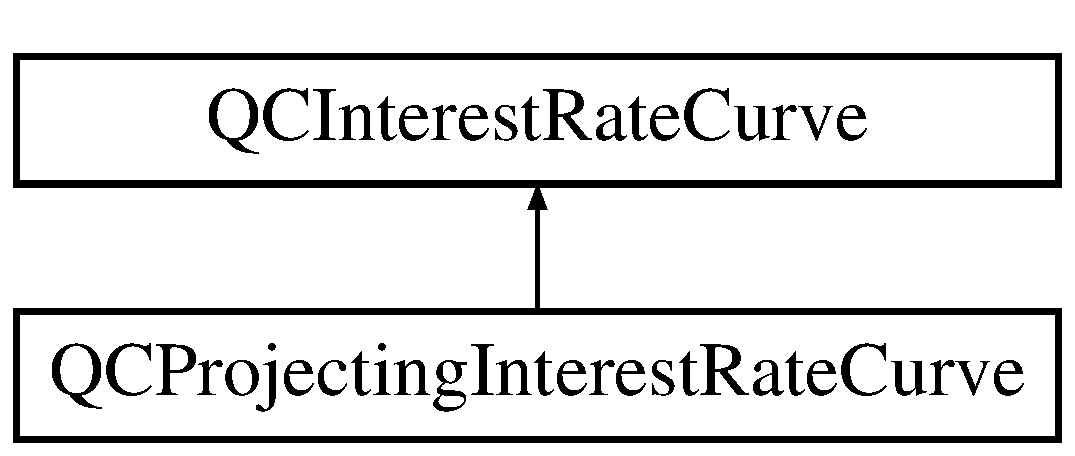
\includegraphics[height=2.000000cm]{class_q_c_projecting_interest_rate_curve}
\end{center}
\end{figure}
\subsection*{Public Member Functions}
\begin{DoxyCompactItemize}
\item 
\hypertarget{class_q_c_projecting_interest_rate_curve_a0f1053cb9509354040a90c68b098f570}{{\bfseries Q\+C\+Projecting\+Interest\+Rate\+Curve} (shared\+\_\+ptr$<$ \hyperlink{class_q_c_interpolator}{Q\+C\+Interpolator} $>$ curve, \hyperlink{class_q_c_interest_rate}{Q\+C\+Interest\+Rate} int\+Rate)}\label{class_q_c_projecting_interest_rate_curve_a0f1053cb9509354040a90c68b098f570}

\item 
virtual double \hyperlink{class_q_c_projecting_interest_rate_curve_af2f420b0178d8a86b67e9d800ec96c8e}{get\+Rate\+At} (long d) override
\item 
virtual double \hyperlink{class_q_c_projecting_interest_rate_curve_a777da5100b3dd412e9764c6129c6715b}{get\+Discount\+Factor\+At} (long d) override
\item 
virtual double \hyperlink{class_q_c_projecting_interest_rate_curve_a2f01098cb4e3c2ba6163fb9bef4a6b66}{get\+Forward\+Rate} (\hyperlink{class_q_c_interest_rate}{Q\+C\+Interest\+Rate} \&int\+Rate, long d1, long d2) override
\item 
virtual double \hyperlink{class_q_c_projecting_interest_rate_curve_a07a0b96ca283abb7f3e0a79432bcdee9}{get\+Forward\+Rate} (long d1, long d2) override
\item 
virtual double \hyperlink{class_q_c_projecting_interest_rate_curve_af58caeb654c8b7623716997d39e96045}{get\+Forward\+Wf} (long d1, long d2) override
\item 
virtual double \hyperlink{class_q_c_projecting_interest_rate_curve_aa32b5f4d4bea4565e3610bda00ed8d06}{df\+Derivative\+At} (unsigned int index) override
\item 
virtual double \hyperlink{class_q_c_projecting_interest_rate_curve_ad6b67e23665886cdcf91957fe12e10d8}{fwd\+Wf\+Derivative\+At} (unsigned int index) override
\end{DoxyCompactItemize}
\subsection*{Additional Inherited Members}


\subsection{Detailed Description}
class \hyperlink{class_q_c_projecting_interest_rate_curve}{Q\+C\+Projecting\+Interest\+Rate\+Curve} Clase que modela curvas de proyeccion modernas donde la tasa fwd se obtiene directamente como un punto interpolado de la curva sin usar factores de descuento fwd. 

Definition at line 12 of file Q\+C\+Projecting\+Interest\+Rate\+Curve.\+h.



\subsection{Member Function Documentation}
\hypertarget{class_q_c_projecting_interest_rate_curve_aa32b5f4d4bea4565e3610bda00ed8d06}{\index{Q\+C\+Projecting\+Interest\+Rate\+Curve@{Q\+C\+Projecting\+Interest\+Rate\+Curve}!df\+Derivative\+At@{df\+Derivative\+At}}
\index{df\+Derivative\+At@{df\+Derivative\+At}!Q\+C\+Projecting\+Interest\+Rate\+Curve@{Q\+C\+Projecting\+Interest\+Rate\+Curve}}
\subsubsection[{df\+Derivative\+At}]{\setlength{\rightskip}{0pt plus 5cm}virtual double Q\+C\+Projecting\+Interest\+Rate\+Curve\+::df\+Derivative\+At (
\begin{DoxyParamCaption}
\item[{unsigned int}]{index}
\end{DoxyParamCaption}
)\hspace{0.3cm}{\ttfamily [override]}, {\ttfamily [virtual]}}}\label{class_q_c_projecting_interest_rate_curve_aa32b5f4d4bea4565e3610bda00ed8d06}
Este método es un getter que retorna la derivada del último factor de capitalización calculado. \begin{DoxyReturn}{Returns}
valor de la derivada. 
\end{DoxyReturn}


Implements \hyperlink{class_q_c_interest_rate_curve_a07a3e60dc1e7d25a025fc587b055c813}{Q\+C\+Interest\+Rate\+Curve}.

\hypertarget{class_q_c_projecting_interest_rate_curve_ad6b67e23665886cdcf91957fe12e10d8}{\index{Q\+C\+Projecting\+Interest\+Rate\+Curve@{Q\+C\+Projecting\+Interest\+Rate\+Curve}!fwd\+Wf\+Derivative\+At@{fwd\+Wf\+Derivative\+At}}
\index{fwd\+Wf\+Derivative\+At@{fwd\+Wf\+Derivative\+At}!Q\+C\+Projecting\+Interest\+Rate\+Curve@{Q\+C\+Projecting\+Interest\+Rate\+Curve}}
\subsubsection[{fwd\+Wf\+Derivative\+At}]{\setlength{\rightskip}{0pt plus 5cm}virtual double Q\+C\+Projecting\+Interest\+Rate\+Curve\+::fwd\+Wf\+Derivative\+At (
\begin{DoxyParamCaption}
\item[{unsigned int}]{index}
\end{DoxyParamCaption}
)\hspace{0.3cm}{\ttfamily [override]}, {\ttfamily [virtual]}}}\label{class_q_c_projecting_interest_rate_curve_ad6b67e23665886cdcf91957fe12e10d8}
Este método es un getter que retorna la derivada del último factor de capitalización forward calculado. \begin{DoxyReturn}{Returns}
valor de la derivada. 
\end{DoxyReturn}


Implements \hyperlink{class_q_c_interest_rate_curve_a8aa3dcfb5a3ce169094db4e2f0849a94}{Q\+C\+Interest\+Rate\+Curve}.

\hypertarget{class_q_c_projecting_interest_rate_curve_a777da5100b3dd412e9764c6129c6715b}{\index{Q\+C\+Projecting\+Interest\+Rate\+Curve@{Q\+C\+Projecting\+Interest\+Rate\+Curve}!get\+Discount\+Factor\+At@{get\+Discount\+Factor\+At}}
\index{get\+Discount\+Factor\+At@{get\+Discount\+Factor\+At}!Q\+C\+Projecting\+Interest\+Rate\+Curve@{Q\+C\+Projecting\+Interest\+Rate\+Curve}}
\subsubsection[{get\+Discount\+Factor\+At}]{\setlength{\rightskip}{0pt plus 5cm}virtual double Q\+C\+Projecting\+Interest\+Rate\+Curve\+::get\+Discount\+Factor\+At (
\begin{DoxyParamCaption}
\item[{long}]{d}
\end{DoxyParamCaption}
)\hspace{0.3cm}{\ttfamily [override]}, {\ttfamily [virtual]}}}\label{class_q_c_projecting_interest_rate_curve_a777da5100b3dd412e9764c6129c6715b}
Retorna el factor de descuento interpolado al plazo d. 
\begin{DoxyParams}{Parameters}
{\em d} & plazo a interpolar \\
\hline
\end{DoxyParams}
\begin{DoxyReturn}{Returns}
valor del factor de descuento interpolado. 
\end{DoxyReturn}


Implements \hyperlink{class_q_c_interest_rate_curve_abe670a951f0fca2273726d13ce9cda06}{Q\+C\+Interest\+Rate\+Curve}.

\hypertarget{class_q_c_projecting_interest_rate_curve_a2f01098cb4e3c2ba6163fb9bef4a6b66}{\index{Q\+C\+Projecting\+Interest\+Rate\+Curve@{Q\+C\+Projecting\+Interest\+Rate\+Curve}!get\+Forward\+Rate@{get\+Forward\+Rate}}
\index{get\+Forward\+Rate@{get\+Forward\+Rate}!Q\+C\+Projecting\+Interest\+Rate\+Curve@{Q\+C\+Projecting\+Interest\+Rate\+Curve}}
\subsubsection[{get\+Forward\+Rate}]{\setlength{\rightskip}{0pt plus 5cm}virtual double Q\+C\+Projecting\+Interest\+Rate\+Curve\+::get\+Forward\+Rate (
\begin{DoxyParamCaption}
\item[{{\bf Q\+C\+Interest\+Rate} \&}]{int\+Rate, }
\item[{long}]{d1, }
\item[{long}]{d2}
\end{DoxyParamCaption}
)\hspace{0.3cm}{\ttfamily [override]}, {\ttfamily [virtual]}}}\label{class_q_c_projecting_interest_rate_curve_a2f01098cb4e3c2ba6163fb9bef4a6b66}
Retorna la tasa forward entre los plazos d1 y d2 en la convención de int\+Rate. 
\begin{DoxyParams}{Parameters}
{\em int\+Rate} & convención de la tasa forward que se debe calcular. \\
\hline
{\em d1} & plazo más corto de la tasa forward. \\
\hline
{\em d2} & plazo más largo de la tasa forward. \\
\hline
\end{DoxyParams}
\begin{DoxyReturn}{Returns}
valor de la tasa forward calculada. Probablemente este método puede mejorarse haciendo que retorne void y el valor de la tasa forward calculada se almacene dentro de la variable int\+Rate. 
\end{DoxyReturn}


Implements \hyperlink{class_q_c_interest_rate_curve_a66e79c4ed2e08916f14bbbfb5d1d3c96}{Q\+C\+Interest\+Rate\+Curve}.

\hypertarget{class_q_c_projecting_interest_rate_curve_a07a0b96ca283abb7f3e0a79432bcdee9}{\index{Q\+C\+Projecting\+Interest\+Rate\+Curve@{Q\+C\+Projecting\+Interest\+Rate\+Curve}!get\+Forward\+Rate@{get\+Forward\+Rate}}
\index{get\+Forward\+Rate@{get\+Forward\+Rate}!Q\+C\+Projecting\+Interest\+Rate\+Curve@{Q\+C\+Projecting\+Interest\+Rate\+Curve}}
\subsubsection[{get\+Forward\+Rate}]{\setlength{\rightskip}{0pt plus 5cm}virtual double Q\+C\+Projecting\+Interest\+Rate\+Curve\+::get\+Forward\+Rate (
\begin{DoxyParamCaption}
\item[{long}]{d1, }
\item[{long}]{d2}
\end{DoxyParamCaption}
)\hspace{0.3cm}{\ttfamily [override]}, {\ttfamily [virtual]}}}\label{class_q_c_projecting_interest_rate_curve_a07a0b96ca283abb7f3e0a79432bcdee9}
Retorna la tasa forward entre los plazos d1 y d2 en la convención de las tasas de la curva. 
\begin{DoxyParams}{Parameters}
{\em d1} & plazo más corto de la tasa forward. \\
\hline
{\em d2} & plazo más largo de la tasa forward. \\
\hline
\end{DoxyParams}
\begin{DoxyReturn}{Returns}
valor de la tasa forward calculada. 
\end{DoxyReturn}


Implements \hyperlink{class_q_c_interest_rate_curve_af4c22b08db379ea8ce825f9999e2bc34}{Q\+C\+Interest\+Rate\+Curve}.

\hypertarget{class_q_c_projecting_interest_rate_curve_af58caeb654c8b7623716997d39e96045}{\index{Q\+C\+Projecting\+Interest\+Rate\+Curve@{Q\+C\+Projecting\+Interest\+Rate\+Curve}!get\+Forward\+Wf@{get\+Forward\+Wf}}
\index{get\+Forward\+Wf@{get\+Forward\+Wf}!Q\+C\+Projecting\+Interest\+Rate\+Curve@{Q\+C\+Projecting\+Interest\+Rate\+Curve}}
\subsubsection[{get\+Forward\+Wf}]{\setlength{\rightskip}{0pt plus 5cm}virtual double Q\+C\+Projecting\+Interest\+Rate\+Curve\+::get\+Forward\+Wf (
\begin{DoxyParamCaption}
\item[{long}]{d1, }
\item[{long}]{d2}
\end{DoxyParamCaption}
)\hspace{0.3cm}{\ttfamily [override]}, {\ttfamily [virtual]}}}\label{class_q_c_projecting_interest_rate_curve_af58caeb654c8b7623716997d39e96045}
Retorna la factor de capitalización forward entre los plazos d1 y d2. 
\begin{DoxyParams}{Parameters}
{\em d1} & plazo más corto del factor forward. \\
\hline
{\em d2} & plazo más largo del fcator forward. \\
\hline
\end{DoxyParams}
\begin{DoxyReturn}{Returns}
valor del factor forward calculado. 
\end{DoxyReturn}


Implements \hyperlink{class_q_c_interest_rate_curve_a36c88024727170486082197f1abff78e}{Q\+C\+Interest\+Rate\+Curve}.

\hypertarget{class_q_c_projecting_interest_rate_curve_af2f420b0178d8a86b67e9d800ec96c8e}{\index{Q\+C\+Projecting\+Interest\+Rate\+Curve@{Q\+C\+Projecting\+Interest\+Rate\+Curve}!get\+Rate\+At@{get\+Rate\+At}}
\index{get\+Rate\+At@{get\+Rate\+At}!Q\+C\+Projecting\+Interest\+Rate\+Curve@{Q\+C\+Projecting\+Interest\+Rate\+Curve}}
\subsubsection[{get\+Rate\+At}]{\setlength{\rightskip}{0pt plus 5cm}virtual double Q\+C\+Projecting\+Interest\+Rate\+Curve\+::get\+Rate\+At (
\begin{DoxyParamCaption}
\item[{long}]{d}
\end{DoxyParamCaption}
)\hspace{0.3cm}{\ttfamily [override]}, {\ttfamily [virtual]}}}\label{class_q_c_projecting_interest_rate_curve_af2f420b0178d8a86b67e9d800ec96c8e}
Retorna la tasa interpolada al plazo d. 
\begin{DoxyParams}{Parameters}
{\em d} & plazo a interpolar \\
\hline
\end{DoxyParams}
\begin{DoxyReturn}{Returns}
valor de la tasa interpolada en la convención de las tasas de la curva. 
\end{DoxyReturn}


Implements \hyperlink{class_q_c_interest_rate_curve_a0a73e8506d0706becd93b04c4499a9c6}{Q\+C\+Interest\+Rate\+Curve}.



The documentation for this class was generated from the following file\+:\begin{DoxyCompactItemize}
\item 
include/Q\+C\+Projecting\+Interest\+Rate\+Curve.\+h\end{DoxyCompactItemize}

\hypertarget{class_q_c_test}{\section{Q\+C\+Test Class Reference}
\label{class_q_c_test}\index{Q\+C\+Test@{Q\+C\+Test}}
}
\subsection*{Public Member Functions}
\begin{DoxyCompactItemize}
\item 
\hypertarget{class_q_c_test_a4514a7e167dc3a413d6fa7dcf0a8bf93}{double {\bfseries suma} (double x, double y)}\label{class_q_c_test_a4514a7e167dc3a413d6fa7dcf0a8bf93}

\end{DoxyCompactItemize}


\subsection{Detailed Description}


Definition at line 4 of file Q\+C\+Test.\+h.



The documentation for this class was generated from the following file\+:\begin{DoxyCompactItemize}
\item 
include/Q\+C\+Test.\+h\end{DoxyCompactItemize}

\hypertarget{class_q_c_wealth_factor}{\section{Q\+C\+Wealth\+Factor Class Reference}
\label{class_q_c_wealth_factor}\index{Q\+C\+Wealth\+Factor@{Q\+C\+Wealth\+Factor}}
}


La clase \hyperlink{class_q_c_wealth_factor}{Q\+C\+Wealth\+Factor} es una clase base. Al subclasearla se implementa un cálculo de factor de capitalización específico como compuesto o lineal. Esta clase es virtual pura.  




{\ttfamily \#include $<$Q\+C\+Wealth\+Factor.\+h$>$}

Inheritance diagram for Q\+C\+Wealth\+Factor\+:\begin{figure}[H]
\begin{center}
\leavevmode
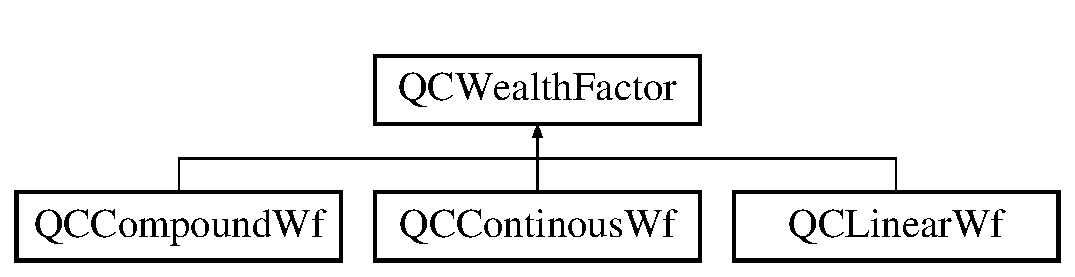
\includegraphics[height=2.000000cm]{class_q_c_wealth_factor}
\end{center}
\end{figure}
\subsection*{Public Member Functions}
\begin{DoxyCompactItemize}
\item 
\hyperlink{class_q_c_wealth_factor_ae2963649c5562d4a05db49825bf1bb15}{Q\+C\+Wealth\+Factor} ()
\item 
virtual double \hyperlink{class_q_c_wealth_factor_a63ddc9c957aa438c1278b541f6e1ebbe}{wf} (double \hyperlink{class_q_c_wealth_factor_aad4a3d84f0c2073162cc5fcce5509d1c}{rate}, double yf)=0
\item 
virtual double \hyperlink{class_q_c_wealth_factor_aad4a3d84f0c2073162cc5fcce5509d1c}{rate} (double \hyperlink{class_q_c_wealth_factor_a63ddc9c957aa438c1278b541f6e1ebbe}{wf}, double yf)=0
\item 
double \hyperlink{class_q_c_wealth_factor_a16a17fd769e2f7945aa1e7925d3f9ace}{dwf} ()
\item 
virtual \hyperlink{class_q_c_wealth_factor_a6ea119054c89d5adb318711ff9452113}{$\sim$\+Q\+C\+Wealth\+Factor} ()
\end{DoxyCompactItemize}
\subsection*{Protected Attributes}
\begin{DoxyCompactItemize}
\item 
double \hyperlink{class_q_c_wealth_factor_ae8552209cdb2f98cd7c3f5011ffe5208}{\+\_\+dwf}
\end{DoxyCompactItemize}


\subsection{Detailed Description}
La clase \hyperlink{class_q_c_wealth_factor}{Q\+C\+Wealth\+Factor} es una clase base. Al subclasearla se implementa un cálculo de factor de capitalización específico como compuesto o lineal. Esta clase es virtual pura. 

\begin{DoxyAuthor}{Author}
Alvaro Díaz 
\end{DoxyAuthor}


Definition at line 11 of file Q\+C\+Wealth\+Factor.\+h.



\subsection{Constructor \& Destructor Documentation}
\hypertarget{class_q_c_wealth_factor_ae2963649c5562d4a05db49825bf1bb15}{\index{Q\+C\+Wealth\+Factor@{Q\+C\+Wealth\+Factor}!Q\+C\+Wealth\+Factor@{Q\+C\+Wealth\+Factor}}
\index{Q\+C\+Wealth\+Factor@{Q\+C\+Wealth\+Factor}!Q\+C\+Wealth\+Factor@{Q\+C\+Wealth\+Factor}}
\subsubsection[{Q\+C\+Wealth\+Factor}]{\setlength{\rightskip}{0pt plus 5cm}Q\+C\+Wealth\+Factor\+::\+Q\+C\+Wealth\+Factor (
\begin{DoxyParamCaption}
{}
\end{DoxyParamCaption}
)}}\label{class_q_c_wealth_factor_ae2963649c5562d4a05db49825bf1bb15}
Constructor por default de la clase \hypertarget{class_q_c_wealth_factor_a6ea119054c89d5adb318711ff9452113}{\index{Q\+C\+Wealth\+Factor@{Q\+C\+Wealth\+Factor}!````~Q\+C\+Wealth\+Factor@{$\sim$\+Q\+C\+Wealth\+Factor}}
\index{````~Q\+C\+Wealth\+Factor@{$\sim$\+Q\+C\+Wealth\+Factor}!Q\+C\+Wealth\+Factor@{Q\+C\+Wealth\+Factor}}
\subsubsection[{$\sim$\+Q\+C\+Wealth\+Factor}]{\setlength{\rightskip}{0pt plus 5cm}virtual Q\+C\+Wealth\+Factor\+::$\sim$\+Q\+C\+Wealth\+Factor (
\begin{DoxyParamCaption}
{}
\end{DoxyParamCaption}
)\hspace{0.3cm}{\ttfamily [virtual]}}}\label{class_q_c_wealth_factor_a6ea119054c89d5adb318711ff9452113}
Destructor de la clase 

\subsection{Member Function Documentation}
\hypertarget{class_q_c_wealth_factor_a16a17fd769e2f7945aa1e7925d3f9ace}{\index{Q\+C\+Wealth\+Factor@{Q\+C\+Wealth\+Factor}!dwf@{dwf}}
\index{dwf@{dwf}!Q\+C\+Wealth\+Factor@{Q\+C\+Wealth\+Factor}}
\subsubsection[{dwf}]{\setlength{\rightskip}{0pt plus 5cm}double Q\+C\+Wealth\+Factor\+::dwf (
\begin{DoxyParamCaption}
{}
\end{DoxyParamCaption}
)}}\label{class_q_c_wealth_factor_a16a17fd769e2f7945aa1e7925d3f9ace}
La función dwf es un getter que devuelve el valor de la derivada del último factor de capitalización calculado, respecto a la tasa. El cálculo de la derivada se realiza al invocar el método wf. \begin{DoxyReturn}{Returns}
(double) valor de la derivada respecto a la tasa 
\end{DoxyReturn}
\hypertarget{class_q_c_wealth_factor_aad4a3d84f0c2073162cc5fcce5509d1c}{\index{Q\+C\+Wealth\+Factor@{Q\+C\+Wealth\+Factor}!rate@{rate}}
\index{rate@{rate}!Q\+C\+Wealth\+Factor@{Q\+C\+Wealth\+Factor}}
\subsubsection[{rate}]{\setlength{\rightskip}{0pt plus 5cm}virtual double Q\+C\+Wealth\+Factor\+::rate (
\begin{DoxyParamCaption}
\item[{double}]{wf, }
\item[{double}]{yf}
\end{DoxyParamCaption}
)\hspace{0.3cm}{\ttfamily [pure virtual]}}}\label{class_q_c_wealth_factor_aad4a3d84f0c2073162cc5fcce5509d1c}
La función rate devuelve el valor de la tasa asociada al valor del factor de capitalización y su fracción de año asociada. 
\begin{DoxyParams}{Parameters}
{\em wf} & es el valor del factor de capitalización \\
\hline
{\em yf} & es el valor de la fracción de año \\
\hline
\end{DoxyParams}
\begin{DoxyReturn}{Returns}
(double) valor de la tasa asociada 
\end{DoxyReturn}


Implemented in \hyperlink{class_q_c_linear_wf_ad0a049fd92a36cecd4b766b181a3cf7b}{Q\+C\+Linear\+Wf}, \hyperlink{class_q_c_compound_wf_a49832a3141f59a281e1ccc8396724bb8}{Q\+C\+Compound\+Wf}, and \hyperlink{class_q_c_continous_wf_addd920e12675b08c941c791e09ceca4a}{Q\+C\+Continous\+Wf}.

\hypertarget{class_q_c_wealth_factor_a63ddc9c957aa438c1278b541f6e1ebbe}{\index{Q\+C\+Wealth\+Factor@{Q\+C\+Wealth\+Factor}!wf@{wf}}
\index{wf@{wf}!Q\+C\+Wealth\+Factor@{Q\+C\+Wealth\+Factor}}
\subsubsection[{wf}]{\setlength{\rightskip}{0pt plus 5cm}virtual double Q\+C\+Wealth\+Factor\+::wf (
\begin{DoxyParamCaption}
\item[{double}]{rate, }
\item[{double}]{yf}
\end{DoxyParamCaption}
)\hspace{0.3cm}{\ttfamily [pure virtual]}}}\label{class_q_c_wealth_factor_a63ddc9c957aa438c1278b541f6e1ebbe}
La función wf devuelve el valor del factor de capitalización dado el valor de una tasa y su fracción de año asociada. Cuando se invoca este método, también se calcula la derivada del factor de capitalización respecto al parámetro rate. Este valor se almacena en la variable protected \+\_\+dwf 
\begin{DoxyParams}{Parameters}
{\em rate} & es el valor de la tasa \\
\hline
{\em yf} & es el valor de la fracción de año \\
\hline
\end{DoxyParams}
\begin{DoxyReturn}{Returns}
(double) valor del factor de capitalización 
\end{DoxyReturn}


Implemented in \hyperlink{class_q_c_linear_wf_ad9ac92ae46857a060f47ceda4291bd72}{Q\+C\+Linear\+Wf}, \hyperlink{class_q_c_compound_wf_a96e3c92f84af47a241a4e24ad470536a}{Q\+C\+Compound\+Wf}, and \hyperlink{class_q_c_continous_wf_a0384d407c9dc90c1579b0ba53d881d5d}{Q\+C\+Continous\+Wf}.



\subsection{Member Data Documentation}
\hypertarget{class_q_c_wealth_factor_ae8552209cdb2f98cd7c3f5011ffe5208}{\index{Q\+C\+Wealth\+Factor@{Q\+C\+Wealth\+Factor}!\+\_\+dwf@{\+\_\+dwf}}
\index{\+\_\+dwf@{\+\_\+dwf}!Q\+C\+Wealth\+Factor@{Q\+C\+Wealth\+Factor}}
\subsubsection[{\+\_\+dwf}]{\setlength{\rightskip}{0pt plus 5cm}double Q\+C\+Wealth\+Factor\+::\+\_\+dwf\hspace{0.3cm}{\ttfamily [protected]}}}\label{class_q_c_wealth_factor_ae8552209cdb2f98cd7c3f5011ffe5208}
Variable protected donde se almacena el valor de la derivada del último factor de capitalización calculado. 

Definition at line 56 of file Q\+C\+Wealth\+Factor.\+h.



The documentation for this class was generated from the following file\+:\begin{DoxyCompactItemize}
\item 
include/Q\+C\+Wealth\+Factor.\+h\end{DoxyCompactItemize}

\hypertarget{class_q_c_year_fraction}{\section{Q\+C\+Year\+Fraction Class Reference}
\label{class_q_c_year_fraction}\index{Q\+C\+Year\+Fraction@{Q\+C\+Year\+Fraction}}
}


La clase \hyperlink{class_q_c_year_fraction}{Q\+C\+Year\+Fraction} es una clase base. Al subclasearla se implementa un cálculo de fracción de año específico como Act/365 o 30/360. Esta clase no se debe instanciar ya que todos sus métodos retornan cero.  




{\ttfamily \#include $<$Q\+C\+Year\+Fraction.\+h$>$}

Inheritance diagram for Q\+C\+Year\+Fraction\+:\begin{figure}[H]
\begin{center}
\leavevmode
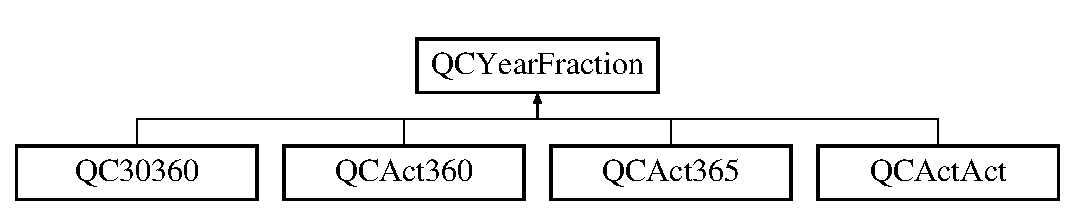
\includegraphics[height=2.000000cm]{class_q_c_year_fraction}
\end{center}
\end{figure}
\subsection*{Public Member Functions}
\begin{DoxyCompactItemize}
\item 
virtual double \hyperlink{class_q_c_year_fraction_abf6d0f4b18d13ce6d31104332511c200}{yf} (const \hyperlink{class_q_c_date}{Q\+C\+Date} \&first\+Date, const \hyperlink{class_q_c_date}{Q\+C\+Date} \&second\+Date)
\item 
virtual long \hyperlink{class_q_c_year_fraction_aca9bd1b20d467d0a516bd19f0ef680e7}{count\+Days} (const \hyperlink{class_q_c_date}{Q\+C\+Date} \&first\+Date, const \hyperlink{class_q_c_date}{Q\+C\+Date} \&second\+Date)
\item 
virtual double \hyperlink{class_q_c_year_fraction_ac8ae7d0408e01f1e58d8ab6afe1ced3f}{yf} (long days)
\end{DoxyCompactItemize}


\subsection{Detailed Description}
La clase \hyperlink{class_q_c_year_fraction}{Q\+C\+Year\+Fraction} es una clase base. Al subclasearla se implementa un cálculo de fracción de año específico como Act/365 o 30/360. Esta clase no se debe instanciar ya que todos sus métodos retornan cero. 

\begin{DoxyAuthor}{Author}
Alvaro Díaz 
\end{DoxyAuthor}


Definition at line 13 of file Q\+C\+Year\+Fraction.\+h.



\subsection{Member Function Documentation}
\hypertarget{class_q_c_year_fraction_aca9bd1b20d467d0a516bd19f0ef680e7}{\index{Q\+C\+Year\+Fraction@{Q\+C\+Year\+Fraction}!count\+Days@{count\+Days}}
\index{count\+Days@{count\+Days}!Q\+C\+Year\+Fraction@{Q\+C\+Year\+Fraction}}
\subsubsection[{count\+Days}]{\setlength{\rightskip}{0pt plus 5cm}virtual long Q\+C\+Year\+Fraction\+::count\+Days (
\begin{DoxyParamCaption}
\item[{const {\bf Q\+C\+Date} \&}]{first\+Date, }
\item[{const {\bf Q\+C\+Date} \&}]{second\+Date}
\end{DoxyParamCaption}
)\hspace{0.3cm}{\ttfamily [inline]}, {\ttfamily [virtual]}}}\label{class_q_c_year_fraction_aca9bd1b20d467d0a516bd19f0ef680e7}
La función count\+Days devuelve el número de días entre first\+Date y second\+Date. Si se desea un número positivo first\+Date debe ser menor que second\+Date 
\begin{DoxyParams}{Parameters}
{\em first\+Date} & es la fecha más antigua de las dos si se desea retornar un valor positivo \\
\hline
{\em second\+Date} & es la fecha más reciente de las dos si se desea retornar un valor positivo \\
\hline
\end{DoxyParams}
\begin{DoxyReturn}{Returns}
(long) con el número de días calculados 
\end{DoxyReturn}


Reimplemented in \hyperlink{class_q_c_act_act_a8d6cc524bd04550d07e1dc1f143e53e7}{Q\+C\+Act\+Act}, \hyperlink{class_q_c_act360_a415e4b5c9d5b5e5b1b9a3fd52795016b}{Q\+C\+Act360}, \hyperlink{class_q_c_act365_a56509add10cf3573bd568390d1035d0b}{Q\+C\+Act365}, and \hyperlink{class_q_c30360_a84ce06c39d386055dc91e43602e4d9e7}{Q\+C30360}.



Definition at line 30 of file Q\+C\+Year\+Fraction.\+h.

\hypertarget{class_q_c_year_fraction_abf6d0f4b18d13ce6d31104332511c200}{\index{Q\+C\+Year\+Fraction@{Q\+C\+Year\+Fraction}!yf@{yf}}
\index{yf@{yf}!Q\+C\+Year\+Fraction@{Q\+C\+Year\+Fraction}}
\subsubsection[{yf}]{\setlength{\rightskip}{0pt plus 5cm}virtual double Q\+C\+Year\+Fraction\+::yf (
\begin{DoxyParamCaption}
\item[{const {\bf Q\+C\+Date} \&}]{first\+Date, }
\item[{const {\bf Q\+C\+Date} \&}]{second\+Date}
\end{DoxyParamCaption}
)\hspace{0.3cm}{\ttfamily [inline]}, {\ttfamily [virtual]}}}\label{class_q_c_year_fraction_abf6d0f4b18d13ce6d31104332511c200}
La función yf devuelve la fracción de año entre dos fechas. 
\begin{DoxyParams}{Parameters}
{\em first\+Date} & es la fecha más antigua de las dos si se desea retornar un valor positivo \\
\hline
{\em second\+Date} & es la fecha más reciente de las dos si se desea retornar un valor positivo \\
\hline
\end{DoxyParams}
\begin{DoxyReturn}{Returns}
(double) con la fracción de año calculada 
\end{DoxyReturn}


Reimplemented in \hyperlink{class_q_c30360_a4db09c9e51398c7b1bf99059d2d83094}{Q\+C30360}, \hyperlink{class_q_c_act_act_aa939d5d44744ffca64e36e3e9d2600bd}{Q\+C\+Act\+Act}, \hyperlink{class_q_c_act360_a63b8c11fddd7949ad0cfa2280ca229e9}{Q\+C\+Act360}, and \hyperlink{class_q_c_act365_ae9ef9155b65718a4e7af7c706c576d95}{Q\+C\+Act365}.



Definition at line 22 of file Q\+C\+Year\+Fraction.\+h.

\hypertarget{class_q_c_year_fraction_ac8ae7d0408e01f1e58d8ab6afe1ced3f}{\index{Q\+C\+Year\+Fraction@{Q\+C\+Year\+Fraction}!yf@{yf}}
\index{yf@{yf}!Q\+C\+Year\+Fraction@{Q\+C\+Year\+Fraction}}
\subsubsection[{yf}]{\setlength{\rightskip}{0pt plus 5cm}virtual double Q\+C\+Year\+Fraction\+::yf (
\begin{DoxyParamCaption}
\item[{long}]{days}
\end{DoxyParamCaption}
)\hspace{0.3cm}{\ttfamily [inline]}, {\ttfamily [virtual]}}}\label{class_q_c_year_fraction_ac8ae7d0408e01f1e58d8ab6afe1ced3f}
Esta sobrecarga de la función yf devuelve un proxy de la fracción de año cuando el argumento es un numero de dias. 
\begin{DoxyParams}{Parameters}
{\em days} & \\
\hline
\end{DoxyParams}
\begin{DoxyReturn}{Returns}
(double) con la fracción de año calculada 
\end{DoxyReturn}


Reimplemented in \hyperlink{class_q_c30360_a9e7776fc765df31d5b60e8f7f87d4d55}{Q\+C30360}, \hyperlink{class_q_c_act_act_ad22ae23fc988e029b70ac05db37b30fc}{Q\+C\+Act\+Act}, \hyperlink{class_q_c_act360_a103e41364093ca0d0157d5782b88dec4}{Q\+C\+Act360}, and \hyperlink{class_q_c_act365_a9579bfd75fece5fbd5391a57348f6d1e}{Q\+C\+Act365}.



Definition at line 37 of file Q\+C\+Year\+Fraction.\+h.



The documentation for this class was generated from the following file\+:\begin{DoxyCompactItemize}
\item 
include/Q\+C\+Year\+Fraction.\+h\end{DoxyCompactItemize}

\hypertarget{class_q_c_zero_coupon_curve}{\section{Q\+C\+Zero\+Coupon\+Curve Class Reference}
\label{class_q_c_zero_coupon_curve}\index{Q\+C\+Zero\+Coupon\+Curve@{Q\+C\+Zero\+Coupon\+Curve}}
}


Clase base (abstracta) para todas las curvas de tasas de interes que son curvas cero cupon.  




{\ttfamily \#include $<$Q\+C\+Zero\+Coupon\+Curve.\+h$>$}

Inheritance diagram for Q\+C\+Zero\+Coupon\+Curve\+:\begin{figure}[H]
\begin{center}
\leavevmode
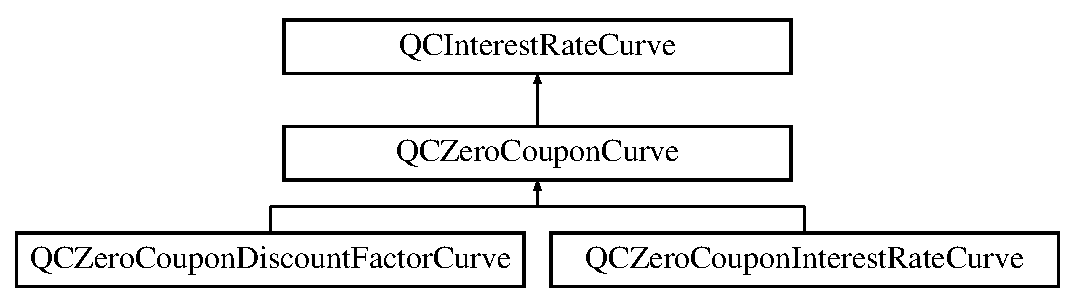
\includegraphics[height=3.000000cm]{class_q_c_zero_coupon_curve}
\end{center}
\end{figure}
\subsection*{Public Member Functions}
\begin{DoxyCompactItemize}
\item 
\hypertarget{class_q_c_zero_coupon_curve_a10de10b602b24f3d9bc73fbbe87f8e35}{{\bfseries Q\+C\+Zero\+Coupon\+Curve} (shared\+\_\+ptr$<$ \hyperlink{class_q_c_interpolator}{Q\+C\+Interpolator} $>$ curve, \hyperlink{class_q_c_interest_rate}{Q\+C\+Interest\+Rate} int\+Rate)}\label{class_q_c_zero_coupon_curve_a10de10b602b24f3d9bc73fbbe87f8e35}

\item 
virtual double \hyperlink{class_q_c_zero_coupon_curve_a83289d8e7ef3cacdc407820b715d9b19}{get\+Rate\+At} (long d)
\item 
virtual double \hyperlink{class_q_c_zero_coupon_curve_ac7546a18d2fe462e14ddae2d8c87b7c5}{get\+Discount\+Factor\+At} (long d)
\item 
\hypertarget{class_q_c_zero_coupon_curve_afebbe4bb5a7b76f3914842c212704fc1}{virtual double {\bfseries get\+Discount\+Factor\+Fwd} (long d1, long d2)}\label{class_q_c_zero_coupon_curve_afebbe4bb5a7b76f3914842c212704fc1}

\item 
\hypertarget{class_q_c_zero_coupon_curve_afa4667c45b9f07890f2ea4dd194c7470}{virtual double {\bfseries get\+Instant\+Forward\+Rate\+At} (long d)}\label{class_q_c_zero_coupon_curve_afa4667c45b9f07890f2ea4dd194c7470}

\item 
\hypertarget{class_q_c_zero_coupon_curve_a10067b1cccec8446ad5d540d69605d42}{virtual double {\bfseries get\+Deriv\+Instant\+Forward\+Rate\+At} (long d)}\label{class_q_c_zero_coupon_curve_a10067b1cccec8446ad5d540d69605d42}

\item 
virtual double \hyperlink{class_q_c_zero_coupon_curve_afe641c34018bcc867b498f67e7c7d19d}{df\+Derivative\+At} (unsigned int index)
\end{DoxyCompactItemize}
\subsection*{Additional Inherited Members}


\subsection{Detailed Description}
Clase base (abstracta) para todas las curvas de tasas de interes que son curvas cero cupon. 

class \hyperlink{class_q_c_interest_rate_curve}{Q\+C\+Interest\+Rate\+Curve}

Esta clase solo define metodos adicionales (obtener una tasas dado un plazo) que todas sus clases derivadas deben override. 

Definition at line 17 of file Q\+C\+Zero\+Coupon\+Curve.\+h.



\subsection{Member Function Documentation}
\hypertarget{class_q_c_zero_coupon_curve_afe641c34018bcc867b498f67e7c7d19d}{\index{Q\+C\+Zero\+Coupon\+Curve@{Q\+C\+Zero\+Coupon\+Curve}!df\+Derivative\+At@{df\+Derivative\+At}}
\index{df\+Derivative\+At@{df\+Derivative\+At}!Q\+C\+Zero\+Coupon\+Curve@{Q\+C\+Zero\+Coupon\+Curve}}
\subsubsection[{df\+Derivative\+At}]{\setlength{\rightskip}{0pt plus 5cm}virtual double Q\+C\+Zero\+Coupon\+Curve\+::df\+Derivative\+At (
\begin{DoxyParamCaption}
\item[{unsigned int}]{index}
\end{DoxyParamCaption}
)\hspace{0.3cm}{\ttfamily [virtual]}}}\label{class_q_c_zero_coupon_curve_afe641c34018bcc867b498f67e7c7d19d}
Este método es un getter que retorna la derivada del último factor de capitalización calculado. \begin{DoxyReturn}{Returns}
valor de la derivada. 
\end{DoxyReturn}


Implements \hyperlink{class_q_c_interest_rate_curve_a07a3e60dc1e7d25a025fc587b055c813}{Q\+C\+Interest\+Rate\+Curve}.



Reimplemented in \hyperlink{class_q_c_zero_coupon_interest_rate_curve_a24ae7f1a9021c24984c5c002d0df1494}{Q\+C\+Zero\+Coupon\+Interest\+Rate\+Curve}.

\hypertarget{class_q_c_zero_coupon_curve_ac7546a18d2fe462e14ddae2d8c87b7c5}{\index{Q\+C\+Zero\+Coupon\+Curve@{Q\+C\+Zero\+Coupon\+Curve}!get\+Discount\+Factor\+At@{get\+Discount\+Factor\+At}}
\index{get\+Discount\+Factor\+At@{get\+Discount\+Factor\+At}!Q\+C\+Zero\+Coupon\+Curve@{Q\+C\+Zero\+Coupon\+Curve}}
\subsubsection[{get\+Discount\+Factor\+At}]{\setlength{\rightskip}{0pt plus 5cm}virtual double Q\+C\+Zero\+Coupon\+Curve\+::get\+Discount\+Factor\+At (
\begin{DoxyParamCaption}
\item[{long}]{d}
\end{DoxyParamCaption}
)\hspace{0.3cm}{\ttfamily [virtual]}}}\label{class_q_c_zero_coupon_curve_ac7546a18d2fe462e14ddae2d8c87b7c5}
Retorna el factor de descuento interpolado al plazo d. 
\begin{DoxyParams}{Parameters}
{\em d} & plazo a interpolar \\
\hline
\end{DoxyParams}
\begin{DoxyReturn}{Returns}
valor del factor de descuento interpolado. 
\end{DoxyReturn}


Implements \hyperlink{class_q_c_interest_rate_curve_abe670a951f0fca2273726d13ce9cda06}{Q\+C\+Interest\+Rate\+Curve}.



Reimplemented in \hyperlink{class_q_c_zero_coupon_discount_factor_curve_a1c09de3cfa88c80f8ece2feac6905c0d}{Q\+C\+Zero\+Coupon\+Discount\+Factor\+Curve}, and \hyperlink{class_q_c_zero_coupon_interest_rate_curve_af3a5bec430ce4a652831b47ccbcca354}{Q\+C\+Zero\+Coupon\+Interest\+Rate\+Curve}.

\hypertarget{class_q_c_zero_coupon_curve_a83289d8e7ef3cacdc407820b715d9b19}{\index{Q\+C\+Zero\+Coupon\+Curve@{Q\+C\+Zero\+Coupon\+Curve}!get\+Rate\+At@{get\+Rate\+At}}
\index{get\+Rate\+At@{get\+Rate\+At}!Q\+C\+Zero\+Coupon\+Curve@{Q\+C\+Zero\+Coupon\+Curve}}
\subsubsection[{get\+Rate\+At}]{\setlength{\rightskip}{0pt plus 5cm}virtual double Q\+C\+Zero\+Coupon\+Curve\+::get\+Rate\+At (
\begin{DoxyParamCaption}
\item[{long}]{d}
\end{DoxyParamCaption}
)\hspace{0.3cm}{\ttfamily [virtual]}}}\label{class_q_c_zero_coupon_curve_a83289d8e7ef3cacdc407820b715d9b19}
Retorna la tasa interpolada al plazo d. 
\begin{DoxyParams}{Parameters}
{\em d} & plazo a interpolar \\
\hline
\end{DoxyParams}
\begin{DoxyReturn}{Returns}
valor de la tasa interpolada en la convención de las tasas de la curva. 
\end{DoxyReturn}


Implements \hyperlink{class_q_c_interest_rate_curve_a0a73e8506d0706becd93b04c4499a9c6}{Q\+C\+Interest\+Rate\+Curve}.



Reimplemented in \hyperlink{class_q_c_zero_coupon_discount_factor_curve_a00da6a6176e027de613935504683e254}{Q\+C\+Zero\+Coupon\+Discount\+Factor\+Curve}, and \hyperlink{class_q_c_zero_coupon_interest_rate_curve_a7841822e2b1291753582dd4ec92269e2}{Q\+C\+Zero\+Coupon\+Interest\+Rate\+Curve}.



The documentation for this class was generated from the following file\+:\begin{DoxyCompactItemize}
\item 
include/Q\+C\+Zero\+Coupon\+Curve.\+h\end{DoxyCompactItemize}

\hypertarget{class_q_c_zero_coupon_discount_factor_curve}{\section{Q\+C\+Zero\+Coupon\+Discount\+Factor\+Curve Class Reference}
\label{class_q_c_zero_coupon_discount_factor_curve}\index{Q\+C\+Zero\+Coupon\+Discount\+Factor\+Curve@{Q\+C\+Zero\+Coupon\+Discount\+Factor\+Curve}}
}
Inheritance diagram for Q\+C\+Zero\+Coupon\+Discount\+Factor\+Curve\+:\begin{figure}[H]
\begin{center}
\leavevmode
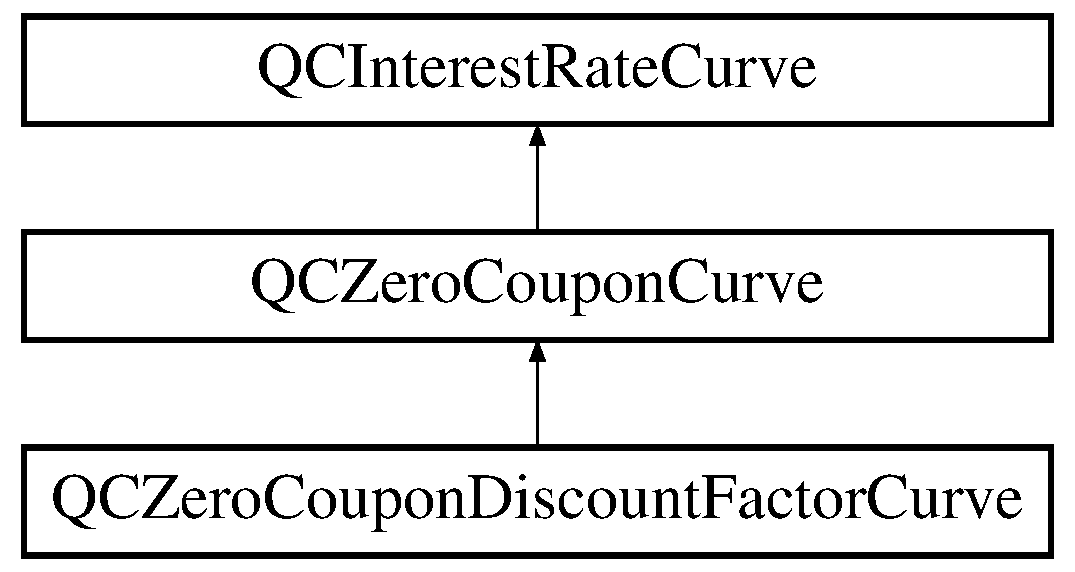
\includegraphics[height=3.000000cm]{class_q_c_zero_coupon_discount_factor_curve}
\end{center}
\end{figure}
\subsection*{Public Member Functions}
\begin{DoxyCompactItemize}
\item 
\hypertarget{class_q_c_zero_coupon_discount_factor_curve_a25350242d9f5a47d8b271d77dcbbc61c}{{\bfseries Q\+C\+Zero\+Coupon\+Discount\+Factor\+Curve} (shared\+\_\+ptr$<$ \hyperlink{class_q_c_interpolator}{Q\+C\+Interpolator} $>$ curve, \hyperlink{class_q_c_interest_rate}{Q\+C\+Interest\+Rate} int\+Rate)}\label{class_q_c_zero_coupon_discount_factor_curve_a25350242d9f5a47d8b271d77dcbbc61c}

\item 
virtual double \hyperlink{class_q_c_zero_coupon_discount_factor_curve_a00da6a6176e027de613935504683e254}{get\+Rate\+At} (long d) override
\item 
virtual double \hyperlink{class_q_c_zero_coupon_discount_factor_curve_a1c09de3cfa88c80f8ece2feac6905c0d}{get\+Discount\+Factor\+At} (long d) override
\item 
\hypertarget{class_q_c_zero_coupon_discount_factor_curve_a9befe6e28f78e8d5e634914a953d0acb}{virtual double {\bfseries get\+Discount\+Factor\+Fwd} (long d1, long d2) override}\label{class_q_c_zero_coupon_discount_factor_curve_a9befe6e28f78e8d5e634914a953d0acb}

\item 
virtual double \hyperlink{class_q_c_zero_coupon_discount_factor_curve_a444623664ba1bd0d0855bc11cbde64dd}{get\+Forward\+Rate} (\hyperlink{class_q_c_interest_rate}{Q\+C\+Interest\+Rate} \&int\+Rate, long d1, long d2) override
\item 
virtual double \hyperlink{class_q_c_zero_coupon_discount_factor_curve_a9287f90424bfa40964835df46d3e3601}{get\+Forward\+Rate} (long d1, long d2) override
\item 
virtual double \hyperlink{class_q_c_zero_coupon_discount_factor_curve_ab9b135fa9deab14e415f95d619c1bfae}{get\+Forward\+Wf} (long d1, long d2) override
\item 
\hypertarget{class_q_c_zero_coupon_discount_factor_curve_a906f9c8951880ed584e8104168fdf14d}{virtual double {\bfseries get\+Instant\+Forward\+Rate\+At} (long d) override}\label{class_q_c_zero_coupon_discount_factor_curve_a906f9c8951880ed584e8104168fdf14d}

\item 
\hypertarget{class_q_c_zero_coupon_discount_factor_curve_aeb4a1654dbec9d763e9b9c00dfeb62a7}{virtual double {\bfseries get\+Deriv\+Instant\+Forward\+Rate\+At} (long d) override}\label{class_q_c_zero_coupon_discount_factor_curve_aeb4a1654dbec9d763e9b9c00dfeb62a7}

\item 
virtual double \hyperlink{class_q_c_zero_coupon_discount_factor_curve_a336906041380286ee1f8257d9a97e486}{fwd\+Wf\+Derivative\+At} (unsigned int index) override
\end{DoxyCompactItemize}
\subsection*{Additional Inherited Members}


\subsection{Detailed Description}


Definition at line 7 of file Q\+C\+Zero\+Coupon\+Discount\+Factor\+Curve.\+h.



\subsection{Member Function Documentation}
\hypertarget{class_q_c_zero_coupon_discount_factor_curve_a336906041380286ee1f8257d9a97e486}{\index{Q\+C\+Zero\+Coupon\+Discount\+Factor\+Curve@{Q\+C\+Zero\+Coupon\+Discount\+Factor\+Curve}!fwd\+Wf\+Derivative\+At@{fwd\+Wf\+Derivative\+At}}
\index{fwd\+Wf\+Derivative\+At@{fwd\+Wf\+Derivative\+At}!Q\+C\+Zero\+Coupon\+Discount\+Factor\+Curve@{Q\+C\+Zero\+Coupon\+Discount\+Factor\+Curve}}
\subsubsection[{fwd\+Wf\+Derivative\+At}]{\setlength{\rightskip}{0pt plus 5cm}virtual double Q\+C\+Zero\+Coupon\+Discount\+Factor\+Curve\+::fwd\+Wf\+Derivative\+At (
\begin{DoxyParamCaption}
\item[{unsigned int}]{index}
\end{DoxyParamCaption}
)\hspace{0.3cm}{\ttfamily [override]}, {\ttfamily [virtual]}}}\label{class_q_c_zero_coupon_discount_factor_curve_a336906041380286ee1f8257d9a97e486}
Este método es un getter que retorna la derivada del último factor de capitalización forward calculado. \begin{DoxyReturn}{Returns}
valor de la derivada. 
\end{DoxyReturn}


Implements \hyperlink{class_q_c_interest_rate_curve_a8aa3dcfb5a3ce169094db4e2f0849a94}{Q\+C\+Interest\+Rate\+Curve}.

\hypertarget{class_q_c_zero_coupon_discount_factor_curve_a1c09de3cfa88c80f8ece2feac6905c0d}{\index{Q\+C\+Zero\+Coupon\+Discount\+Factor\+Curve@{Q\+C\+Zero\+Coupon\+Discount\+Factor\+Curve}!get\+Discount\+Factor\+At@{get\+Discount\+Factor\+At}}
\index{get\+Discount\+Factor\+At@{get\+Discount\+Factor\+At}!Q\+C\+Zero\+Coupon\+Discount\+Factor\+Curve@{Q\+C\+Zero\+Coupon\+Discount\+Factor\+Curve}}
\subsubsection[{get\+Discount\+Factor\+At}]{\setlength{\rightskip}{0pt plus 5cm}virtual double Q\+C\+Zero\+Coupon\+Discount\+Factor\+Curve\+::get\+Discount\+Factor\+At (
\begin{DoxyParamCaption}
\item[{long}]{d}
\end{DoxyParamCaption}
)\hspace{0.3cm}{\ttfamily [override]}, {\ttfamily [virtual]}}}\label{class_q_c_zero_coupon_discount_factor_curve_a1c09de3cfa88c80f8ece2feac6905c0d}
Retorna el factor de descuento interpolado al plazo d. 
\begin{DoxyParams}{Parameters}
{\em d} & plazo a interpolar \\
\hline
\end{DoxyParams}
\begin{DoxyReturn}{Returns}
valor del factor de descuento interpolado. 
\end{DoxyReturn}


Reimplemented from \hyperlink{class_q_c_zero_coupon_curve_ac7546a18d2fe462e14ddae2d8c87b7c5}{Q\+C\+Zero\+Coupon\+Curve}.

\hypertarget{class_q_c_zero_coupon_discount_factor_curve_a444623664ba1bd0d0855bc11cbde64dd}{\index{Q\+C\+Zero\+Coupon\+Discount\+Factor\+Curve@{Q\+C\+Zero\+Coupon\+Discount\+Factor\+Curve}!get\+Forward\+Rate@{get\+Forward\+Rate}}
\index{get\+Forward\+Rate@{get\+Forward\+Rate}!Q\+C\+Zero\+Coupon\+Discount\+Factor\+Curve@{Q\+C\+Zero\+Coupon\+Discount\+Factor\+Curve}}
\subsubsection[{get\+Forward\+Rate}]{\setlength{\rightskip}{0pt plus 5cm}virtual double Q\+C\+Zero\+Coupon\+Discount\+Factor\+Curve\+::get\+Forward\+Rate (
\begin{DoxyParamCaption}
\item[{{\bf Q\+C\+Interest\+Rate} \&}]{int\+Rate, }
\item[{long}]{d1, }
\item[{long}]{d2}
\end{DoxyParamCaption}
)\hspace{0.3cm}{\ttfamily [override]}, {\ttfamily [virtual]}}}\label{class_q_c_zero_coupon_discount_factor_curve_a444623664ba1bd0d0855bc11cbde64dd}
Retorna la tasa forward entre los plazos d1 y d2 en la convención de int\+Rate. 
\begin{DoxyParams}{Parameters}
{\em int\+Rate} & convención de la tasa forward que se debe calcular. \\
\hline
{\em d1} & plazo más corto de la tasa forward. \\
\hline
{\em d2} & plazo más largo de la tasa forward. \\
\hline
\end{DoxyParams}
\begin{DoxyReturn}{Returns}
valor de la tasa forward calculada. Probablemente este método puede mejorarse haciendo que retorne void y el valor de la tasa forward calculada se almacene dentro de la variable int\+Rate. 
\end{DoxyReturn}


Implements \hyperlink{class_q_c_interest_rate_curve_a66e79c4ed2e08916f14bbbfb5d1d3c96}{Q\+C\+Interest\+Rate\+Curve}.

\hypertarget{class_q_c_zero_coupon_discount_factor_curve_a9287f90424bfa40964835df46d3e3601}{\index{Q\+C\+Zero\+Coupon\+Discount\+Factor\+Curve@{Q\+C\+Zero\+Coupon\+Discount\+Factor\+Curve}!get\+Forward\+Rate@{get\+Forward\+Rate}}
\index{get\+Forward\+Rate@{get\+Forward\+Rate}!Q\+C\+Zero\+Coupon\+Discount\+Factor\+Curve@{Q\+C\+Zero\+Coupon\+Discount\+Factor\+Curve}}
\subsubsection[{get\+Forward\+Rate}]{\setlength{\rightskip}{0pt plus 5cm}virtual double Q\+C\+Zero\+Coupon\+Discount\+Factor\+Curve\+::get\+Forward\+Rate (
\begin{DoxyParamCaption}
\item[{long}]{d1, }
\item[{long}]{d2}
\end{DoxyParamCaption}
)\hspace{0.3cm}{\ttfamily [override]}, {\ttfamily [virtual]}}}\label{class_q_c_zero_coupon_discount_factor_curve_a9287f90424bfa40964835df46d3e3601}
Retorna la tasa forward entre los plazos d1 y d2 en la convención de las tasas de la curva. 
\begin{DoxyParams}{Parameters}
{\em d1} & plazo más corto de la tasa forward. \\
\hline
{\em d2} & plazo más largo de la tasa forward. \\
\hline
\end{DoxyParams}
\begin{DoxyReturn}{Returns}
valor de la tasa forward calculada. 
\end{DoxyReturn}


Implements \hyperlink{class_q_c_interest_rate_curve_af4c22b08db379ea8ce825f9999e2bc34}{Q\+C\+Interest\+Rate\+Curve}.

\hypertarget{class_q_c_zero_coupon_discount_factor_curve_ab9b135fa9deab14e415f95d619c1bfae}{\index{Q\+C\+Zero\+Coupon\+Discount\+Factor\+Curve@{Q\+C\+Zero\+Coupon\+Discount\+Factor\+Curve}!get\+Forward\+Wf@{get\+Forward\+Wf}}
\index{get\+Forward\+Wf@{get\+Forward\+Wf}!Q\+C\+Zero\+Coupon\+Discount\+Factor\+Curve@{Q\+C\+Zero\+Coupon\+Discount\+Factor\+Curve}}
\subsubsection[{get\+Forward\+Wf}]{\setlength{\rightskip}{0pt plus 5cm}virtual double Q\+C\+Zero\+Coupon\+Discount\+Factor\+Curve\+::get\+Forward\+Wf (
\begin{DoxyParamCaption}
\item[{long}]{d1, }
\item[{long}]{d2}
\end{DoxyParamCaption}
)\hspace{0.3cm}{\ttfamily [override]}, {\ttfamily [virtual]}}}\label{class_q_c_zero_coupon_discount_factor_curve_ab9b135fa9deab14e415f95d619c1bfae}
Retorna la factor de capitalización forward entre los plazos d1 y d2. 
\begin{DoxyParams}{Parameters}
{\em d1} & plazo más corto del factor forward. \\
\hline
{\em d2} & plazo más largo del fcator forward. \\
\hline
\end{DoxyParams}
\begin{DoxyReturn}{Returns}
valor del factor forward calculado. 
\end{DoxyReturn}


Implements \hyperlink{class_q_c_interest_rate_curve_a36c88024727170486082197f1abff78e}{Q\+C\+Interest\+Rate\+Curve}.

\hypertarget{class_q_c_zero_coupon_discount_factor_curve_a00da6a6176e027de613935504683e254}{\index{Q\+C\+Zero\+Coupon\+Discount\+Factor\+Curve@{Q\+C\+Zero\+Coupon\+Discount\+Factor\+Curve}!get\+Rate\+At@{get\+Rate\+At}}
\index{get\+Rate\+At@{get\+Rate\+At}!Q\+C\+Zero\+Coupon\+Discount\+Factor\+Curve@{Q\+C\+Zero\+Coupon\+Discount\+Factor\+Curve}}
\subsubsection[{get\+Rate\+At}]{\setlength{\rightskip}{0pt plus 5cm}virtual double Q\+C\+Zero\+Coupon\+Discount\+Factor\+Curve\+::get\+Rate\+At (
\begin{DoxyParamCaption}
\item[{long}]{d}
\end{DoxyParamCaption}
)\hspace{0.3cm}{\ttfamily [override]}, {\ttfamily [virtual]}}}\label{class_q_c_zero_coupon_discount_factor_curve_a00da6a6176e027de613935504683e254}
Retorna la tasa interpolada al plazo d. 
\begin{DoxyParams}{Parameters}
{\em d} & plazo a interpolar \\
\hline
\end{DoxyParams}
\begin{DoxyReturn}{Returns}
valor de la tasa interpolada en la convención de las tasas de la curva. 
\end{DoxyReturn}


Reimplemented from \hyperlink{class_q_c_zero_coupon_curve_a83289d8e7ef3cacdc407820b715d9b19}{Q\+C\+Zero\+Coupon\+Curve}.



The documentation for this class was generated from the following file\+:\begin{DoxyCompactItemize}
\item 
include/Q\+C\+Zero\+Coupon\+Discount\+Factor\+Curve.\+h\end{DoxyCompactItemize}

\hypertarget{class_q_c_zero_coupon_interest_rate_curve}{\section{Q\+C\+Zero\+Coupon\+Interest\+Rate\+Curve Class Reference}
\label{class_q_c_zero_coupon_interest_rate_curve}\index{Q\+C\+Zero\+Coupon\+Interest\+Rate\+Curve@{Q\+C\+Zero\+Coupon\+Interest\+Rate\+Curve}}
}
Inheritance diagram for Q\+C\+Zero\+Coupon\+Interest\+Rate\+Curve\+:\begin{figure}[H]
\begin{center}
\leavevmode
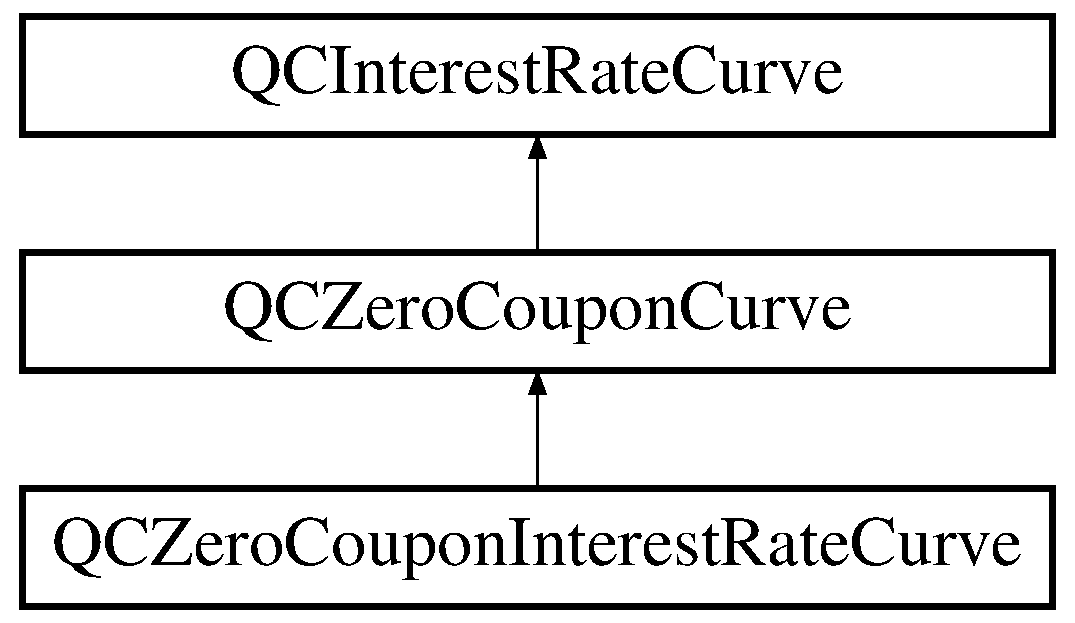
\includegraphics[height=3.000000cm]{class_q_c_zero_coupon_interest_rate_curve}
\end{center}
\end{figure}
\subsection*{Public Member Functions}
\begin{DoxyCompactItemize}
\item 
\hypertarget{class_q_c_zero_coupon_interest_rate_curve_a2fcb4f578bcdff82483a5aa9c7c85bb9}{{\bfseries Q\+C\+Zero\+Coupon\+Interest\+Rate\+Curve} (shared\+\_\+ptr$<$ \hyperlink{class_q_c_interpolator}{Q\+C\+Interpolator} $>$ curve, \hyperlink{class_q_c_interest_rate}{Q\+C\+Interest\+Rate} int\+Rate)}\label{class_q_c_zero_coupon_interest_rate_curve_a2fcb4f578bcdff82483a5aa9c7c85bb9}

\item 
virtual double \hyperlink{class_q_c_zero_coupon_interest_rate_curve_a7841822e2b1291753582dd4ec92269e2}{get\+Rate\+At} (long d) override
\item 
virtual double \hyperlink{class_q_c_zero_coupon_interest_rate_curve_af3a5bec430ce4a652831b47ccbcca354}{get\+Discount\+Factor\+At} (long d) override
\item 
\hypertarget{class_q_c_zero_coupon_interest_rate_curve_aa03c419f97d6551cf05b1d7a9ee6c4e9}{virtual double {\bfseries get\+Discount\+Factor\+Fwd} (long d1, long d2) override}\label{class_q_c_zero_coupon_interest_rate_curve_aa03c419f97d6551cf05b1d7a9ee6c4e9}

\item 
virtual double \hyperlink{class_q_c_zero_coupon_interest_rate_curve_a623b9416cc04c5a2a59b1279f20d3220}{get\+Forward\+Rate} (\hyperlink{class_q_c_interest_rate}{Q\+C\+Interest\+Rate} \&int\+Rate, long d1, long d2) override
\item 
virtual double \hyperlink{class_q_c_zero_coupon_interest_rate_curve_a17770bb86b17de6336be98b622ff992b}{get\+Forward\+Rate} (long d1, long d2) override
\item 
virtual double \hyperlink{class_q_c_zero_coupon_interest_rate_curve_a6da87ca82b003afbc336388c5e7b6eb6}{get\+Forward\+Wf} (long d1, long d2) override
\item 
\hypertarget{class_q_c_zero_coupon_interest_rate_curve_af5b678775f644fff398572ffd5557ec9}{virtual double {\bfseries get\+Instant\+Forward\+Rate\+At} (long d) override}\label{class_q_c_zero_coupon_interest_rate_curve_af5b678775f644fff398572ffd5557ec9}

\item 
\hypertarget{class_q_c_zero_coupon_interest_rate_curve_a97f20476b850350894241c5c3517d9ed}{virtual double {\bfseries get\+Deriv\+Instant\+Forward\+Rate\+At} (long d) override}\label{class_q_c_zero_coupon_interest_rate_curve_a97f20476b850350894241c5c3517d9ed}

\item 
virtual double \hyperlink{class_q_c_zero_coupon_interest_rate_curve_a24ae7f1a9021c24984c5c002d0df1494}{df\+Derivative\+At} (unsigned int index) override
\item 
virtual double \hyperlink{class_q_c_zero_coupon_interest_rate_curve_a043fd0690f9a941b5268e1b1f7d07ef1}{fwd\+Wf\+Derivative\+At} (unsigned int index) override
\end{DoxyCompactItemize}
\subsection*{Additional Inherited Members}


\subsection{Detailed Description}


Definition at line 7 of file Q\+C\+Zero\+Coupon\+Interest\+Rate\+Curve.\+h.



\subsection{Member Function Documentation}
\hypertarget{class_q_c_zero_coupon_interest_rate_curve_a24ae7f1a9021c24984c5c002d0df1494}{\index{Q\+C\+Zero\+Coupon\+Interest\+Rate\+Curve@{Q\+C\+Zero\+Coupon\+Interest\+Rate\+Curve}!df\+Derivative\+At@{df\+Derivative\+At}}
\index{df\+Derivative\+At@{df\+Derivative\+At}!Q\+C\+Zero\+Coupon\+Interest\+Rate\+Curve@{Q\+C\+Zero\+Coupon\+Interest\+Rate\+Curve}}
\subsubsection[{df\+Derivative\+At}]{\setlength{\rightskip}{0pt plus 5cm}virtual double Q\+C\+Zero\+Coupon\+Interest\+Rate\+Curve\+::df\+Derivative\+At (
\begin{DoxyParamCaption}
\item[{unsigned int}]{index}
\end{DoxyParamCaption}
)\hspace{0.3cm}{\ttfamily [override]}, {\ttfamily [virtual]}}}\label{class_q_c_zero_coupon_interest_rate_curve_a24ae7f1a9021c24984c5c002d0df1494}
Este método es un getter que retorna la derivada del último factor de capitalización calculado. \begin{DoxyReturn}{Returns}
valor de la derivada. 
\end{DoxyReturn}


Reimplemented from \hyperlink{class_q_c_zero_coupon_curve_afe641c34018bcc867b498f67e7c7d19d}{Q\+C\+Zero\+Coupon\+Curve}.

\hypertarget{class_q_c_zero_coupon_interest_rate_curve_a043fd0690f9a941b5268e1b1f7d07ef1}{\index{Q\+C\+Zero\+Coupon\+Interest\+Rate\+Curve@{Q\+C\+Zero\+Coupon\+Interest\+Rate\+Curve}!fwd\+Wf\+Derivative\+At@{fwd\+Wf\+Derivative\+At}}
\index{fwd\+Wf\+Derivative\+At@{fwd\+Wf\+Derivative\+At}!Q\+C\+Zero\+Coupon\+Interest\+Rate\+Curve@{Q\+C\+Zero\+Coupon\+Interest\+Rate\+Curve}}
\subsubsection[{fwd\+Wf\+Derivative\+At}]{\setlength{\rightskip}{0pt plus 5cm}virtual double Q\+C\+Zero\+Coupon\+Interest\+Rate\+Curve\+::fwd\+Wf\+Derivative\+At (
\begin{DoxyParamCaption}
\item[{unsigned int}]{index}
\end{DoxyParamCaption}
)\hspace{0.3cm}{\ttfamily [override]}, {\ttfamily [virtual]}}}\label{class_q_c_zero_coupon_interest_rate_curve_a043fd0690f9a941b5268e1b1f7d07ef1}
Este método es un getter que retorna la derivada del último factor de capitalización forward calculado. \begin{DoxyReturn}{Returns}
valor de la derivada. 
\end{DoxyReturn}


Implements \hyperlink{class_q_c_interest_rate_curve_a8aa3dcfb5a3ce169094db4e2f0849a94}{Q\+C\+Interest\+Rate\+Curve}.

\hypertarget{class_q_c_zero_coupon_interest_rate_curve_af3a5bec430ce4a652831b47ccbcca354}{\index{Q\+C\+Zero\+Coupon\+Interest\+Rate\+Curve@{Q\+C\+Zero\+Coupon\+Interest\+Rate\+Curve}!get\+Discount\+Factor\+At@{get\+Discount\+Factor\+At}}
\index{get\+Discount\+Factor\+At@{get\+Discount\+Factor\+At}!Q\+C\+Zero\+Coupon\+Interest\+Rate\+Curve@{Q\+C\+Zero\+Coupon\+Interest\+Rate\+Curve}}
\subsubsection[{get\+Discount\+Factor\+At}]{\setlength{\rightskip}{0pt plus 5cm}virtual double Q\+C\+Zero\+Coupon\+Interest\+Rate\+Curve\+::get\+Discount\+Factor\+At (
\begin{DoxyParamCaption}
\item[{long}]{d}
\end{DoxyParamCaption}
)\hspace{0.3cm}{\ttfamily [override]}, {\ttfamily [virtual]}}}\label{class_q_c_zero_coupon_interest_rate_curve_af3a5bec430ce4a652831b47ccbcca354}
Retorna el factor de descuento interpolado al plazo d. 
\begin{DoxyParams}{Parameters}
{\em d} & plazo a interpolar \\
\hline
\end{DoxyParams}
\begin{DoxyReturn}{Returns}
valor del factor de descuento interpolado. 
\end{DoxyReturn}


Reimplemented from \hyperlink{class_q_c_zero_coupon_curve_ac7546a18d2fe462e14ddae2d8c87b7c5}{Q\+C\+Zero\+Coupon\+Curve}.

\hypertarget{class_q_c_zero_coupon_interest_rate_curve_a623b9416cc04c5a2a59b1279f20d3220}{\index{Q\+C\+Zero\+Coupon\+Interest\+Rate\+Curve@{Q\+C\+Zero\+Coupon\+Interest\+Rate\+Curve}!get\+Forward\+Rate@{get\+Forward\+Rate}}
\index{get\+Forward\+Rate@{get\+Forward\+Rate}!Q\+C\+Zero\+Coupon\+Interest\+Rate\+Curve@{Q\+C\+Zero\+Coupon\+Interest\+Rate\+Curve}}
\subsubsection[{get\+Forward\+Rate}]{\setlength{\rightskip}{0pt plus 5cm}virtual double Q\+C\+Zero\+Coupon\+Interest\+Rate\+Curve\+::get\+Forward\+Rate (
\begin{DoxyParamCaption}
\item[{{\bf Q\+C\+Interest\+Rate} \&}]{int\+Rate, }
\item[{long}]{d1, }
\item[{long}]{d2}
\end{DoxyParamCaption}
)\hspace{0.3cm}{\ttfamily [override]}, {\ttfamily [virtual]}}}\label{class_q_c_zero_coupon_interest_rate_curve_a623b9416cc04c5a2a59b1279f20d3220}
Retorna la tasa forward entre los plazos d1 y d2 en la convención de int\+Rate. 
\begin{DoxyParams}{Parameters}
{\em int\+Rate} & convención de la tasa forward que se debe calcular. \\
\hline
{\em d1} & plazo más corto de la tasa forward. \\
\hline
{\em d2} & plazo más largo de la tasa forward. \\
\hline
\end{DoxyParams}
\begin{DoxyReturn}{Returns}
valor de la tasa forward calculada. Probablemente este método puede mejorarse haciendo que retorne void y el valor de la tasa forward calculada se almacene dentro de la variable int\+Rate. 
\end{DoxyReturn}


Implements \hyperlink{class_q_c_interest_rate_curve_a66e79c4ed2e08916f14bbbfb5d1d3c96}{Q\+C\+Interest\+Rate\+Curve}.

\hypertarget{class_q_c_zero_coupon_interest_rate_curve_a17770bb86b17de6336be98b622ff992b}{\index{Q\+C\+Zero\+Coupon\+Interest\+Rate\+Curve@{Q\+C\+Zero\+Coupon\+Interest\+Rate\+Curve}!get\+Forward\+Rate@{get\+Forward\+Rate}}
\index{get\+Forward\+Rate@{get\+Forward\+Rate}!Q\+C\+Zero\+Coupon\+Interest\+Rate\+Curve@{Q\+C\+Zero\+Coupon\+Interest\+Rate\+Curve}}
\subsubsection[{get\+Forward\+Rate}]{\setlength{\rightskip}{0pt plus 5cm}virtual double Q\+C\+Zero\+Coupon\+Interest\+Rate\+Curve\+::get\+Forward\+Rate (
\begin{DoxyParamCaption}
\item[{long}]{d1, }
\item[{long}]{d2}
\end{DoxyParamCaption}
)\hspace{0.3cm}{\ttfamily [override]}, {\ttfamily [virtual]}}}\label{class_q_c_zero_coupon_interest_rate_curve_a17770bb86b17de6336be98b622ff992b}
Retorna la tasa forward entre los plazos d1 y d2 en la convención de las tasas de la curva. 
\begin{DoxyParams}{Parameters}
{\em d1} & plazo más corto de la tasa forward. \\
\hline
{\em d2} & plazo más largo de la tasa forward. \\
\hline
\end{DoxyParams}
\begin{DoxyReturn}{Returns}
valor de la tasa forward calculada. 
\end{DoxyReturn}


Implements \hyperlink{class_q_c_interest_rate_curve_af4c22b08db379ea8ce825f9999e2bc34}{Q\+C\+Interest\+Rate\+Curve}.

\hypertarget{class_q_c_zero_coupon_interest_rate_curve_a6da87ca82b003afbc336388c5e7b6eb6}{\index{Q\+C\+Zero\+Coupon\+Interest\+Rate\+Curve@{Q\+C\+Zero\+Coupon\+Interest\+Rate\+Curve}!get\+Forward\+Wf@{get\+Forward\+Wf}}
\index{get\+Forward\+Wf@{get\+Forward\+Wf}!Q\+C\+Zero\+Coupon\+Interest\+Rate\+Curve@{Q\+C\+Zero\+Coupon\+Interest\+Rate\+Curve}}
\subsubsection[{get\+Forward\+Wf}]{\setlength{\rightskip}{0pt plus 5cm}virtual double Q\+C\+Zero\+Coupon\+Interest\+Rate\+Curve\+::get\+Forward\+Wf (
\begin{DoxyParamCaption}
\item[{long}]{d1, }
\item[{long}]{d2}
\end{DoxyParamCaption}
)\hspace{0.3cm}{\ttfamily [override]}, {\ttfamily [virtual]}}}\label{class_q_c_zero_coupon_interest_rate_curve_a6da87ca82b003afbc336388c5e7b6eb6}
Retorna la factor de capitalización forward entre los plazos d1 y d2. 
\begin{DoxyParams}{Parameters}
{\em d1} & plazo más corto del factor forward. \\
\hline
{\em d2} & plazo más largo del fcator forward. \\
\hline
\end{DoxyParams}
\begin{DoxyReturn}{Returns}
valor del factor forward calculado. 
\end{DoxyReturn}


Implements \hyperlink{class_q_c_interest_rate_curve_a36c88024727170486082197f1abff78e}{Q\+C\+Interest\+Rate\+Curve}.

\hypertarget{class_q_c_zero_coupon_interest_rate_curve_a7841822e2b1291753582dd4ec92269e2}{\index{Q\+C\+Zero\+Coupon\+Interest\+Rate\+Curve@{Q\+C\+Zero\+Coupon\+Interest\+Rate\+Curve}!get\+Rate\+At@{get\+Rate\+At}}
\index{get\+Rate\+At@{get\+Rate\+At}!Q\+C\+Zero\+Coupon\+Interest\+Rate\+Curve@{Q\+C\+Zero\+Coupon\+Interest\+Rate\+Curve}}
\subsubsection[{get\+Rate\+At}]{\setlength{\rightskip}{0pt plus 5cm}virtual double Q\+C\+Zero\+Coupon\+Interest\+Rate\+Curve\+::get\+Rate\+At (
\begin{DoxyParamCaption}
\item[{long}]{d}
\end{DoxyParamCaption}
)\hspace{0.3cm}{\ttfamily [override]}, {\ttfamily [virtual]}}}\label{class_q_c_zero_coupon_interest_rate_curve_a7841822e2b1291753582dd4ec92269e2}
Retorna la tasa interpolada al plazo d. 
\begin{DoxyParams}{Parameters}
{\em d} & plazo a interpolar \\
\hline
\end{DoxyParams}
\begin{DoxyReturn}{Returns}
valor de la tasa interpolada en la convención de las tasas de la curva. 
\end{DoxyReturn}


Reimplemented from \hyperlink{class_q_c_zero_coupon_curve_a83289d8e7ef3cacdc407820b715d9b19}{Q\+C\+Zero\+Coupon\+Curve}.



The documentation for this class was generated from the following file\+:\begin{DoxyCompactItemize}
\item 
include/Q\+C\+Zero\+Coupon\+Interest\+Rate\+Curve.\+h\end{DoxyCompactItemize}

\chapter{File Documentation}
\hypertarget{_q_c_definitions_8h}{\section{include/\+Q\+C\+Definitions.h File Reference}
\label{_q_c_definitions_8h}\index{include/\+Q\+C\+Definitions.\+h@{include/\+Q\+C\+Definitions.\+h}}
}


Contiene enum y typedef que se usan en otras clases y funciones.  


{\ttfamily \#include $<$memory$>$}\\*
{\ttfamily \#include $<$vector$>$}\\*
{\ttfamily \#include $<$utility$>$}\\*
{\ttfamily \#include $<$tuple$>$}\\*
{\ttfamily \#include $<$map$>$}\\*
{\ttfamily \#include \char`\"{}Q\+C\+Date.\+h\char`\"{}}\\*
\subsection*{Typedefs}
\begin{DoxyCompactItemize}
\item 
typedef shared\+\_\+ptr\\*
$<$ \hyperlink{class_q_c_interest_rate_curve}{Q\+C\+Interest\+Rate\+Curve} $>$ \hyperlink{_q_c_definitions_8h_a4b4fb466e49550e3dfd40003562cd19d}{Q\+C\+Int\+Rt\+Crv\+Shrd\+Ptr}
\item 
typedef shared\+\_\+ptr\\*
$<$ \hyperlink{class_q_c_zero_coupon_curve}{Q\+C\+Zero\+Coupon\+Curve} $>$ \hyperlink{_q_c_definitions_8h_a041384dd6e5600afe47d0ec835a0000f}{Q\+C\+Zr\+Cpn\+Crv\+Shrd\+Ptr}
\item 
typedef shared\+\_\+ptr\\*
$<$ Q\+C\+Discount\+Factor\+Curve $>$ \hyperlink{_q_c_definitions_8h_a2519585063febc023711bce0c5d17b31}{Q\+C\+Disc\+Fctr\+Crv\+Shrd\+Ptr}
\item 
typedef shared\+\_\+ptr\\*
$<$ \hyperlink{class_q_c_interest_rate_payoff}{Q\+C\+Interest\+Rate\+Payoff} $>$ \hyperlink{_q_c_definitions_8h_abf56b288608ba1b455eed753174d29a4}{Q\+C\+Intrst\+Rt\+Pff\+Shrd\+Ptr}
\item 
typedef shared\+\_\+ptr$<$ map\\*
$<$ \hyperlink{class_q_c_date}{Q\+C\+Date}, double $>$ $>$ \hyperlink{_q_c_definitions_8h_a6a601ffd693c05dd81309e3dca08b8f5}{Q\+C\+Time\+Series\+Shrd\+Ptr}
\item 
typedef shared\+\_\+ptr\\*
$<$ \hyperlink{class_q_c_wealth_factor}{Q\+C\+Wealth\+Factor} $>$ \hyperlink{_q_c_definitions_8h_a2085df477a1aafaad6ed79890607f447}{Q\+C\+Wlth\+Fctr\+Shrd\+Ptr}
\item 
typedef shared\+\_\+ptr\\*
$<$ \hyperlink{class_q_c_year_fraction}{Q\+C\+Year\+Fraction} $>$ \hyperlink{_q_c_definitions_8h_abcfd4021c75f633fa6d7a4552ced4a38}{Q\+C\+Yr\+Frctn\+Shrd\+Ptr}
\item 
typedef shared\+\_\+ptr\\*
$<$ \hyperlink{class_q_c_interest_rate}{Q\+C\+Interest\+Rate} $>$ \hyperlink{_q_c_definitions_8h_ae6a21ad26d19e482e3b01179cbc05298}{Q\+C\+Intrst\+Rt\+Shrd\+Ptr}
\item 
typedef tuple$<$ \hyperlink{class_q_c_interest_rate}{Q\+C\+Interest\+Rate} $>$ \hyperlink{_q_c_definitions_8h_a4fc6d76137db7e80b2562f8562798296}{Q\+C\+Fixed\+Leg\+Tuple}
\end{DoxyCompactItemize}
\subsection*{Enumerations}
\begin{DoxyCompactItemize}
\item 
enum \hyperlink{_q_c_definitions_8h_a71276d31176b562a1d8604c5bcb850fc}{Q\+C\+Z\+C\+C\+Representation} \{ \hyperlink{_q_c_definitions_8h_a71276d31176b562a1d8604c5bcb850fca6aceb05608b9d85a54b985499c54a64f}{qc\+Z\+C\+C\+Interest\+Rate}, 
\hyperlink{_q_c_definitions_8h_a71276d31176b562a1d8604c5bcb850fca9bf5d15037a5ad967285aca5746a88a8}{qc\+Z\+C\+C\+Discount\+Factor}, 
\hyperlink{_q_c_definitions_8h_a71276d31176b562a1d8604c5bcb850fca264b4f453fe9dd0fa94b6b1074dcb53a}{qc\+Z\+C\+C\+Wealth\+Factor}
 \}
\end{DoxyCompactItemize}


\subsection{Detailed Description}
Contiene enum y typedef que se usan en otras clases y funciones. 



Definition in file \hyperlink{_q_c_definitions_8h_source}{Q\+C\+Definitions.\+h}.



\subsection{Typedef Documentation}
\hypertarget{_q_c_definitions_8h_a2519585063febc023711bce0c5d17b31}{\index{Q\+C\+Definitions.\+h@{Q\+C\+Definitions.\+h}!Q\+C\+Disc\+Fctr\+Crv\+Shrd\+Ptr@{Q\+C\+Disc\+Fctr\+Crv\+Shrd\+Ptr}}
\index{Q\+C\+Disc\+Fctr\+Crv\+Shrd\+Ptr@{Q\+C\+Disc\+Fctr\+Crv\+Shrd\+Ptr}!Q\+C\+Definitions.\+h@{Q\+C\+Definitions.\+h}}
\subsubsection[{Q\+C\+Disc\+Fctr\+Crv\+Shrd\+Ptr}]{\setlength{\rightskip}{0pt plus 5cm}typedef shared\+\_\+ptr$<$Q\+C\+Discount\+Factor\+Curve$>$ {\bf Q\+C\+Disc\+Fctr\+Crv\+Shrd\+Ptr}}}\label{_q_c_definitions_8h_a2519585063febc023711bce0c5d17b31}
Shared pointer de Q\+C\+Discount\+Factor\+Curve 

Definition at line 49 of file Q\+C\+Definitions.\+h.

\hypertarget{_q_c_definitions_8h_a4fc6d76137db7e80b2562f8562798296}{\index{Q\+C\+Definitions.\+h@{Q\+C\+Definitions.\+h}!Q\+C\+Fixed\+Leg\+Tuple@{Q\+C\+Fixed\+Leg\+Tuple}}
\index{Q\+C\+Fixed\+Leg\+Tuple@{Q\+C\+Fixed\+Leg\+Tuple}!Q\+C\+Definitions.\+h@{Q\+C\+Definitions.\+h}}
\subsubsection[{Q\+C\+Fixed\+Leg\+Tuple}]{\setlength{\rightskip}{0pt plus 5cm}typedef tuple$<${\bf Q\+C\+Interest\+Rate}$>$ {\bf Q\+C\+Fixed\+Leg\+Tuple}}}\label{_q_c_definitions_8h_a4fc6d76137db7e80b2562f8562798296}
Representa en una tupla los elementos de una pata fija que permiten construir el \hyperlink{class_q_c_interest_rate_leg}{Q\+C\+Interest\+Rate\+Leg} asociado 

Definition at line 83 of file Q\+C\+Definitions.\+h.

\hypertarget{_q_c_definitions_8h_abf56b288608ba1b455eed753174d29a4}{\index{Q\+C\+Definitions.\+h@{Q\+C\+Definitions.\+h}!Q\+C\+Intrst\+Rt\+Pff\+Shrd\+Ptr@{Q\+C\+Intrst\+Rt\+Pff\+Shrd\+Ptr}}
\index{Q\+C\+Intrst\+Rt\+Pff\+Shrd\+Ptr@{Q\+C\+Intrst\+Rt\+Pff\+Shrd\+Ptr}!Q\+C\+Definitions.\+h@{Q\+C\+Definitions.\+h}}
\subsubsection[{Q\+C\+Intrst\+Rt\+Pff\+Shrd\+Ptr}]{\setlength{\rightskip}{0pt plus 5cm}typedef shared\+\_\+ptr$<${\bf Q\+C\+Interest\+Rate\+Payoff}$>$ {\bf Q\+C\+Intrst\+Rt\+Pff\+Shrd\+Ptr}}}\label{_q_c_definitions_8h_abf56b288608ba1b455eed753174d29a4}
Shared pointer de \hyperlink{class_q_c_interest_rate_payoff}{Q\+C\+Interest\+Rate\+Payoff} 

Definition at line 54 of file Q\+C\+Definitions.\+h.

\hypertarget{_q_c_definitions_8h_ae6a21ad26d19e482e3b01179cbc05298}{\index{Q\+C\+Definitions.\+h@{Q\+C\+Definitions.\+h}!Q\+C\+Intrst\+Rt\+Shrd\+Ptr@{Q\+C\+Intrst\+Rt\+Shrd\+Ptr}}
\index{Q\+C\+Intrst\+Rt\+Shrd\+Ptr@{Q\+C\+Intrst\+Rt\+Shrd\+Ptr}!Q\+C\+Definitions.\+h@{Q\+C\+Definitions.\+h}}
\subsubsection[{Q\+C\+Intrst\+Rt\+Shrd\+Ptr}]{\setlength{\rightskip}{0pt plus 5cm}typedef shared\+\_\+ptr$<${\bf Q\+C\+Interest\+Rate}$>$ {\bf Q\+C\+Intrst\+Rt\+Shrd\+Ptr}}}\label{_q_c_definitions_8h_ae6a21ad26d19e482e3b01179cbc05298}
Shared pointer de \hyperlink{class_q_c_interest_rate}{Q\+C\+Interest\+Rate} 

Definition at line 77 of file Q\+C\+Definitions.\+h.

\hypertarget{_q_c_definitions_8h_a4b4fb466e49550e3dfd40003562cd19d}{\index{Q\+C\+Definitions.\+h@{Q\+C\+Definitions.\+h}!Q\+C\+Int\+Rt\+Crv\+Shrd\+Ptr@{Q\+C\+Int\+Rt\+Crv\+Shrd\+Ptr}}
\index{Q\+C\+Int\+Rt\+Crv\+Shrd\+Ptr@{Q\+C\+Int\+Rt\+Crv\+Shrd\+Ptr}!Q\+C\+Definitions.\+h@{Q\+C\+Definitions.\+h}}
\subsubsection[{Q\+C\+Int\+Rt\+Crv\+Shrd\+Ptr}]{\setlength{\rightskip}{0pt plus 5cm}typedef shared\+\_\+ptr$<${\bf Q\+C\+Interest\+Rate\+Curve}$>$ {\bf Q\+C\+Int\+Rt\+Crv\+Shrd\+Ptr}}}\label{_q_c_definitions_8h_a4b4fb466e49550e3dfd40003562cd19d}
Shared pointer de \hyperlink{class_q_c_interest_rate_curve}{Q\+C\+Interest\+Rate\+Curve} 

Definition at line 39 of file Q\+C\+Definitions.\+h.

\hypertarget{_q_c_definitions_8h_a6a601ffd693c05dd81309e3dca08b8f5}{\index{Q\+C\+Definitions.\+h@{Q\+C\+Definitions.\+h}!Q\+C\+Time\+Series\+Shrd\+Ptr@{Q\+C\+Time\+Series\+Shrd\+Ptr}}
\index{Q\+C\+Time\+Series\+Shrd\+Ptr@{Q\+C\+Time\+Series\+Shrd\+Ptr}!Q\+C\+Definitions.\+h@{Q\+C\+Definitions.\+h}}
\subsubsection[{Q\+C\+Time\+Series\+Shrd\+Ptr}]{\setlength{\rightskip}{0pt plus 5cm}typedef shared\+\_\+ptr$<$map$<${\bf Q\+C\+Date}, double$>$ $>$ {\bf Q\+C\+Time\+Series\+Shrd\+Ptr}}}\label{_q_c_definitions_8h_a6a601ffd693c05dd81309e3dca08b8f5}
Shared pointer de map$<$\+Q\+C\+Date, double$>$ Este tipo se utiliza para representar un serie de tiempo de un factor de mercado. Por ejemplo, los valores durante un año de la Libor U\+S\+D 3\+M se almacenarían en un objeto de este tipo. 

Definition at line 62 of file Q\+C\+Definitions.\+h.

\hypertarget{_q_c_definitions_8h_a2085df477a1aafaad6ed79890607f447}{\index{Q\+C\+Definitions.\+h@{Q\+C\+Definitions.\+h}!Q\+C\+Wlth\+Fctr\+Shrd\+Ptr@{Q\+C\+Wlth\+Fctr\+Shrd\+Ptr}}
\index{Q\+C\+Wlth\+Fctr\+Shrd\+Ptr@{Q\+C\+Wlth\+Fctr\+Shrd\+Ptr}!Q\+C\+Definitions.\+h@{Q\+C\+Definitions.\+h}}
\subsubsection[{Q\+C\+Wlth\+Fctr\+Shrd\+Ptr}]{\setlength{\rightskip}{0pt plus 5cm}typedef shared\+\_\+ptr$<${\bf Q\+C\+Wealth\+Factor}$>$ {\bf Q\+C\+Wlth\+Fctr\+Shrd\+Ptr}}}\label{_q_c_definitions_8h_a2085df477a1aafaad6ed79890607f447}
Shared pointer de \hyperlink{class_q_c_wealth_factor}{Q\+C\+Wealth\+Factor} 

Definition at line 67 of file Q\+C\+Definitions.\+h.

\hypertarget{_q_c_definitions_8h_abcfd4021c75f633fa6d7a4552ced4a38}{\index{Q\+C\+Definitions.\+h@{Q\+C\+Definitions.\+h}!Q\+C\+Yr\+Frctn\+Shrd\+Ptr@{Q\+C\+Yr\+Frctn\+Shrd\+Ptr}}
\index{Q\+C\+Yr\+Frctn\+Shrd\+Ptr@{Q\+C\+Yr\+Frctn\+Shrd\+Ptr}!Q\+C\+Definitions.\+h@{Q\+C\+Definitions.\+h}}
\subsubsection[{Q\+C\+Yr\+Frctn\+Shrd\+Ptr}]{\setlength{\rightskip}{0pt plus 5cm}typedef shared\+\_\+ptr$<${\bf Q\+C\+Year\+Fraction}$>$ {\bf Q\+C\+Yr\+Frctn\+Shrd\+Ptr}}}\label{_q_c_definitions_8h_abcfd4021c75f633fa6d7a4552ced4a38}
Shared pointer de \hyperlink{class_q_c_year_fraction}{Q\+C\+Year\+Fraction} 

Definition at line 72 of file Q\+C\+Definitions.\+h.

\hypertarget{_q_c_definitions_8h_a041384dd6e5600afe47d0ec835a0000f}{\index{Q\+C\+Definitions.\+h@{Q\+C\+Definitions.\+h}!Q\+C\+Zr\+Cpn\+Crv\+Shrd\+Ptr@{Q\+C\+Zr\+Cpn\+Crv\+Shrd\+Ptr}}
\index{Q\+C\+Zr\+Cpn\+Crv\+Shrd\+Ptr@{Q\+C\+Zr\+Cpn\+Crv\+Shrd\+Ptr}!Q\+C\+Definitions.\+h@{Q\+C\+Definitions.\+h}}
\subsubsection[{Q\+C\+Zr\+Cpn\+Crv\+Shrd\+Ptr}]{\setlength{\rightskip}{0pt plus 5cm}typedef shared\+\_\+ptr$<${\bf Q\+C\+Zero\+Coupon\+Curve}$>$ {\bf Q\+C\+Zr\+Cpn\+Crv\+Shrd\+Ptr}}}\label{_q_c_definitions_8h_a041384dd6e5600afe47d0ec835a0000f}
Shared pointer de \hyperlink{class_q_c_zero_coupon_curve}{Q\+C\+Zero\+Coupon\+Curve} 

Definition at line 44 of file Q\+C\+Definitions.\+h.



\subsection{Enumeration Type Documentation}
\hypertarget{_q_c_definitions_8h_a71276d31176b562a1d8604c5bcb850fc}{\index{Q\+C\+Definitions.\+h@{Q\+C\+Definitions.\+h}!Q\+C\+Z\+C\+C\+Representation@{Q\+C\+Z\+C\+C\+Representation}}
\index{Q\+C\+Z\+C\+C\+Representation@{Q\+C\+Z\+C\+C\+Representation}!Q\+C\+Definitions.\+h@{Q\+C\+Definitions.\+h}}
\subsubsection[{Q\+C\+Z\+C\+C\+Representation}]{\setlength{\rightskip}{0pt plus 5cm}enum {\bf Q\+C\+Z\+C\+C\+Representation}}}\label{_q_c_definitions_8h_a71276d31176b562a1d8604c5bcb850fc}
Enumera las alternativas al dar de alta una curva cero cupon \begin{Desc}
\item[Enumerator]\par
\begin{description}
\index{qc\+Z\+C\+C\+Interest\+Rate@{qc\+Z\+C\+C\+Interest\+Rate}!Q\+C\+Definitions.\+h@{Q\+C\+Definitions.\+h}}\index{Q\+C\+Definitions.\+h@{Q\+C\+Definitions.\+h}!qc\+Z\+C\+C\+Interest\+Rate@{qc\+Z\+C\+C\+Interest\+Rate}}\item[{\em 
\hypertarget{_q_c_definitions_8h_a71276d31176b562a1d8604c5bcb850fca6aceb05608b9d85a54b985499c54a64f}{qc\+Z\+C\+C\+Interest\+Rate}\label{_q_c_definitions_8h_a71276d31176b562a1d8604c5bcb850fca6aceb05608b9d85a54b985499c54a64f}
}]Curva cero cupón se representa con tasas \index{qc\+Z\+C\+C\+Discount\+Factor@{qc\+Z\+C\+C\+Discount\+Factor}!Q\+C\+Definitions.\+h@{Q\+C\+Definitions.\+h}}\index{Q\+C\+Definitions.\+h@{Q\+C\+Definitions.\+h}!qc\+Z\+C\+C\+Discount\+Factor@{qc\+Z\+C\+C\+Discount\+Factor}}\item[{\em 
\hypertarget{_q_c_definitions_8h_a71276d31176b562a1d8604c5bcb850fca9bf5d15037a5ad967285aca5746a88a8}{qc\+Z\+C\+C\+Discount\+Factor}\label{_q_c_definitions_8h_a71276d31176b562a1d8604c5bcb850fca9bf5d15037a5ad967285aca5746a88a8}
}]Curva cero cupón se representa con df \index{qc\+Z\+C\+C\+Wealth\+Factor@{qc\+Z\+C\+C\+Wealth\+Factor}!Q\+C\+Definitions.\+h@{Q\+C\+Definitions.\+h}}\index{Q\+C\+Definitions.\+h@{Q\+C\+Definitions.\+h}!qc\+Z\+C\+C\+Wealth\+Factor@{qc\+Z\+C\+C\+Wealth\+Factor}}\item[{\em 
\hypertarget{_q_c_definitions_8h_a71276d31176b562a1d8604c5bcb850fca264b4f453fe9dd0fa94b6b1074dcb53a}{qc\+Z\+C\+C\+Wealth\+Factor}\label{_q_c_definitions_8h_a71276d31176b562a1d8604c5bcb850fca264b4f453fe9dd0fa94b6b1074dcb53a}
}]Curva cero cupón se representa con wf \end{description}
\end{Desc}


Definition at line 29 of file Q\+C\+Definitions.\+h.


%--- End generated contents ---

% Index
\newpage
\phantomsection
\addcontentsline{toc}{chapter}{Index}
\printindex

\end{document}
